\chapter{初段ミューオントリガーの性能評価}\label{chapter5}
本章では、第~\ref{chapter4}章で述べた手法を用いて作成した2種類のCoincidence~Window(シミュレーション用のCWと実際の測定用のCW)を用いたトリガーの性能の評価を行う。

\section{機械学習を用いて作成したCWの15段階閾値の評価}
便宜上、本研究の手法で作成した2種類のCWについて、シミュレーション用のCWを$\mathrm{CW_{Simu}}$、実際の測定用のCWを$\mathrm{CW_{Data}}$と呼び、比較対象として2022年度Run-3で使用されたCWを$\mathrm{CW_{2022}}$と呼ぶこととする。

\ref{L1Topo}節で述べたL1トリガーには、ミューオンの不変質量を指針としたトリガーを持つL1Topoが存在する。しかし、不変質量を計算するときに使用するミューオンの運動量は、L1Muonから送られてくる$p_{\rm{T}}$閾値であるため、L1Muonの$p_{\rm{T}}$閾値の細かさがそのままL1Topoのトリガー性能に影響する。
そこで、Run-3ではL1Muonにおける判定可能な$p_{\rm{T}}$閾値を6段階から15段階に増設することで、より細かい精度での$p_{\rm{T}}$判定を可能とし、L1トリガー全体としてのトリガー性能の向上を図った。
したがって、本研究で作成するCWにも正確に15段階の$p_{\rm{T}}$判定ができることが要求される。

本節では、全オフライン再構成されたミューオンの内、ある$p_{\rm{T}}$閾値以上のトリガーが発行された割合$\epsilon$を計算し、トリガー効率の算出を行った。また、$\epsilon$をオフライン再構成した$p_{\rm{T}}$の関数として表したTurn-on curveを描き、式~\eqref{equ:fitting}の関数によってフィッティングを行う事で、トリガー性能の評価を行った。
このとき、Tag-And-Probe法を用いて評価に用いるデータの処理を行う。

\subsection{作成したCWの15段階の$p_{\rm{T}}$閾値}
図~\ref{fig:15Eff_CW_Simu}に$\mathrm{CW_{Simu}}$を用いてを要求した15段階の$p_{\rm{T}}$閾値におけるTurn-on curveを示す。評価にはシングルミューオンのシミュレーションサンプルを用いた。
$\mathrm{CW_{2022}}$と同様に、本研究の手法で作成した$\mathrm{CW_{Simu}}$は15段階に分かれたTurn-on curveを描けていることがわかる。
また、図~\ref{fig:15Eff_CW_Data}に$\mathrm{CW_{Data}}$を用いて15段階の$p_{\rm{T}}$閾値におけるTurn-on curveを示す。評価には2018年Run-2 のデータに対して$Z\rightarrow \mu\mu$によるTag-And-Probe法を用いた。
こちらも同様に、本研究の手法で作成した$\mathrm{CW_{Data}}$は15段階に分かれたTurn-on curveを描けていることがわかる。
本研究の手法によって作成された2種類のCWは、2022年度Run-3において使用された$\mathrm{CW_{2022}}$と同様に細かい精度で15段階の判定が可能であり、本研究の手法を用いて15段階の閾値を持ったCWを作成できることが確認できた。
\begin{figure}
    %\centering
    \begin{tabular}{cc}
    \begin{minipage}[b]{0.45\hsize}
        %\centering
        \hspace*{-1cm}
        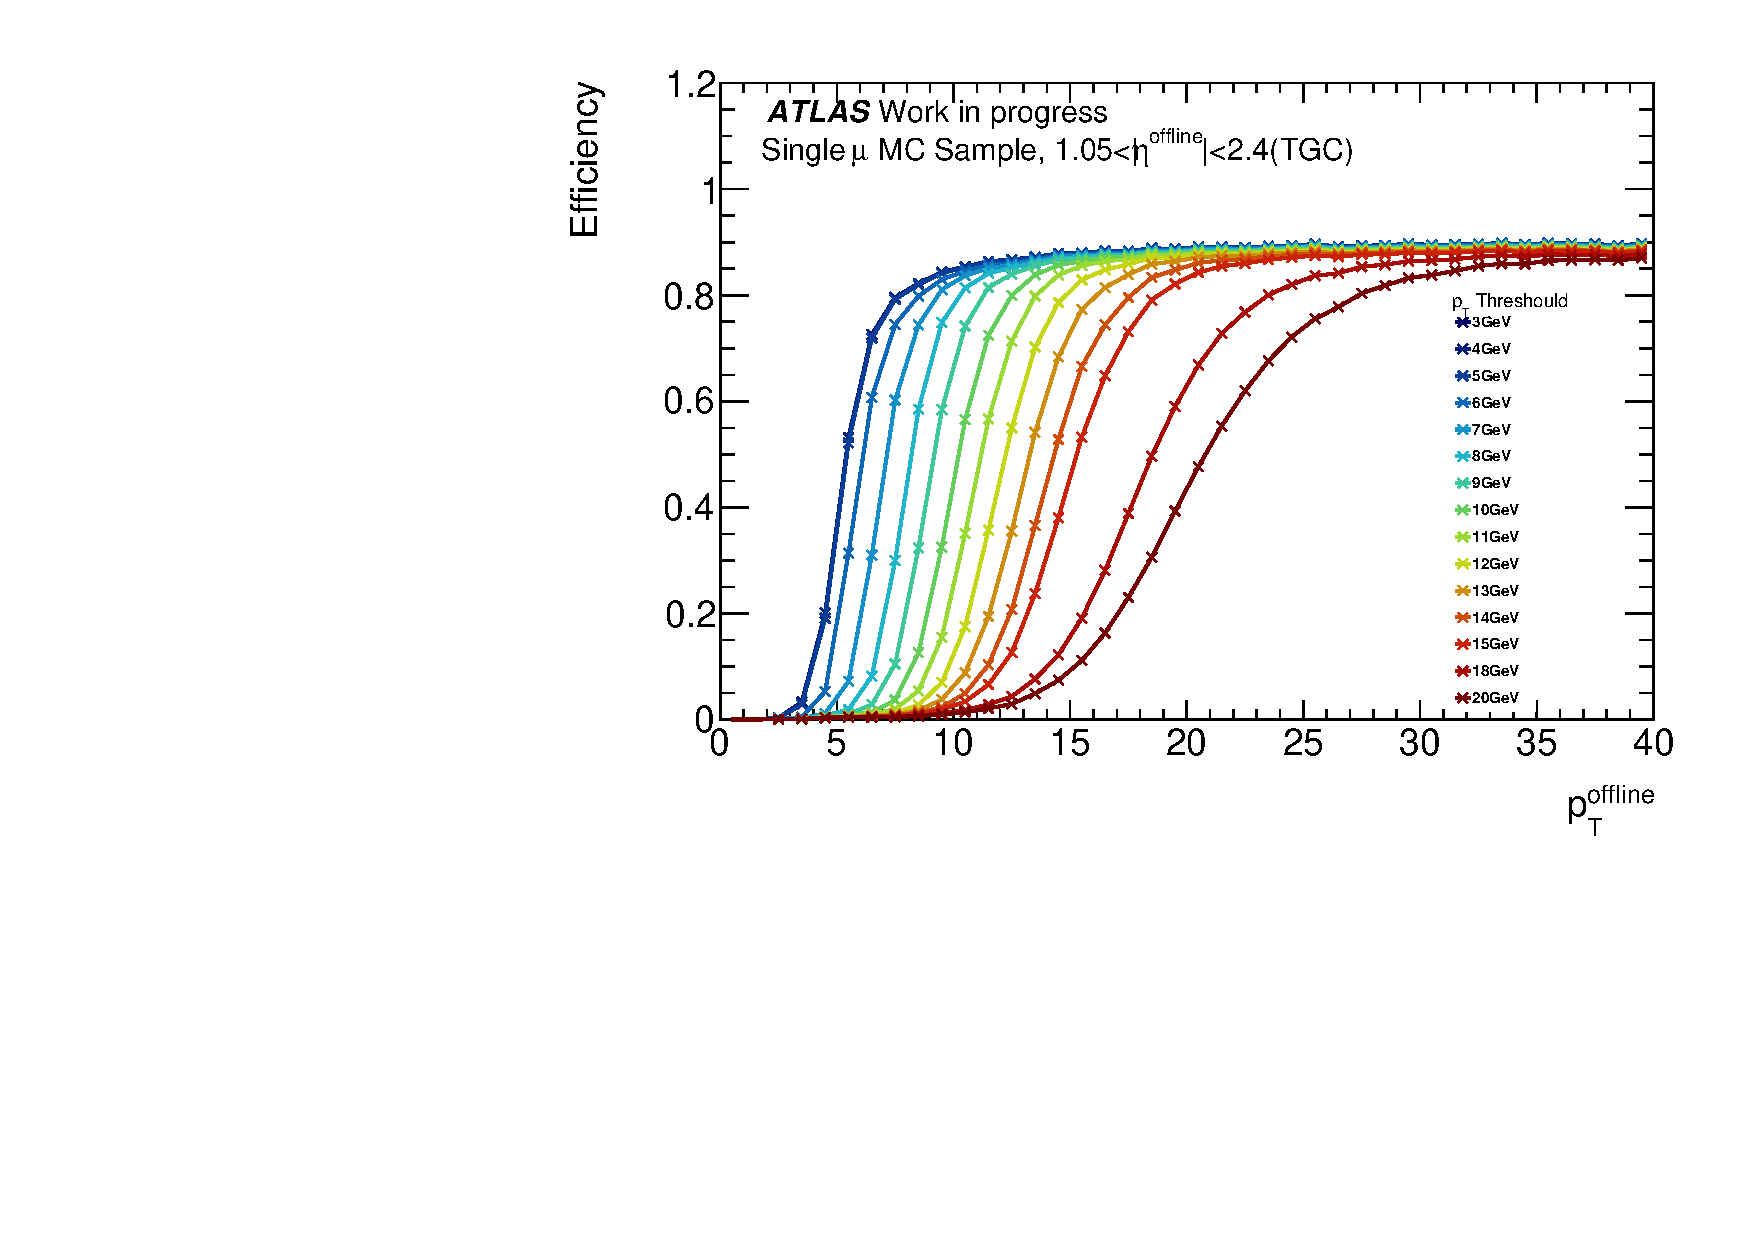
\includegraphics[clip, width=8cm]{fig/5/15_MC_MC_re.pdf}
        %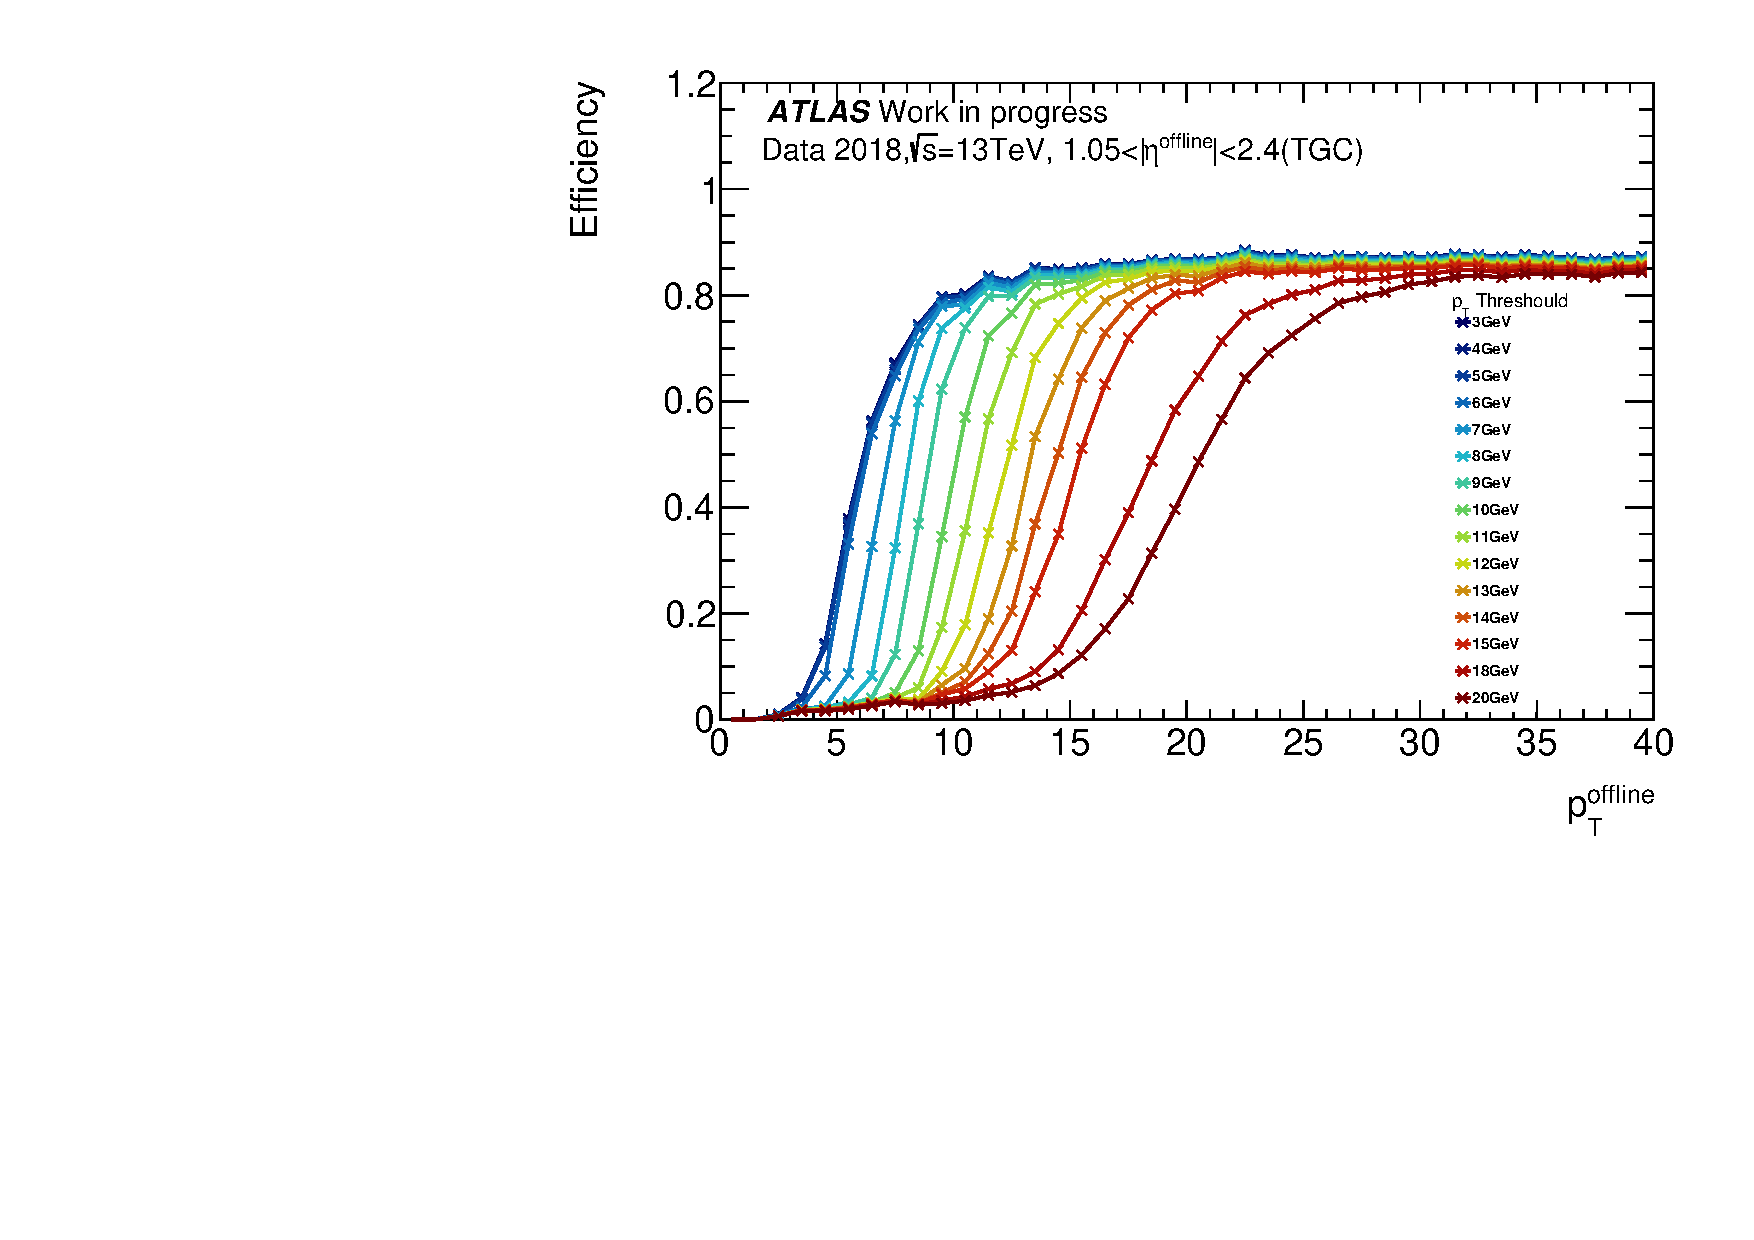
\includegraphics[clip, width=8cm]{fig/5/15_v06_Data.pdf}
        %\vspace{5pt}
        \subcaption{$\mathrm{CW_{Simu}}$のTurn-on curve}
        \label{fig:15Eff_CW_Simu}
    \end{minipage}&
    %\hfill
    \begin{minipage}[b]{0.55\hsize}
        %\centering
        %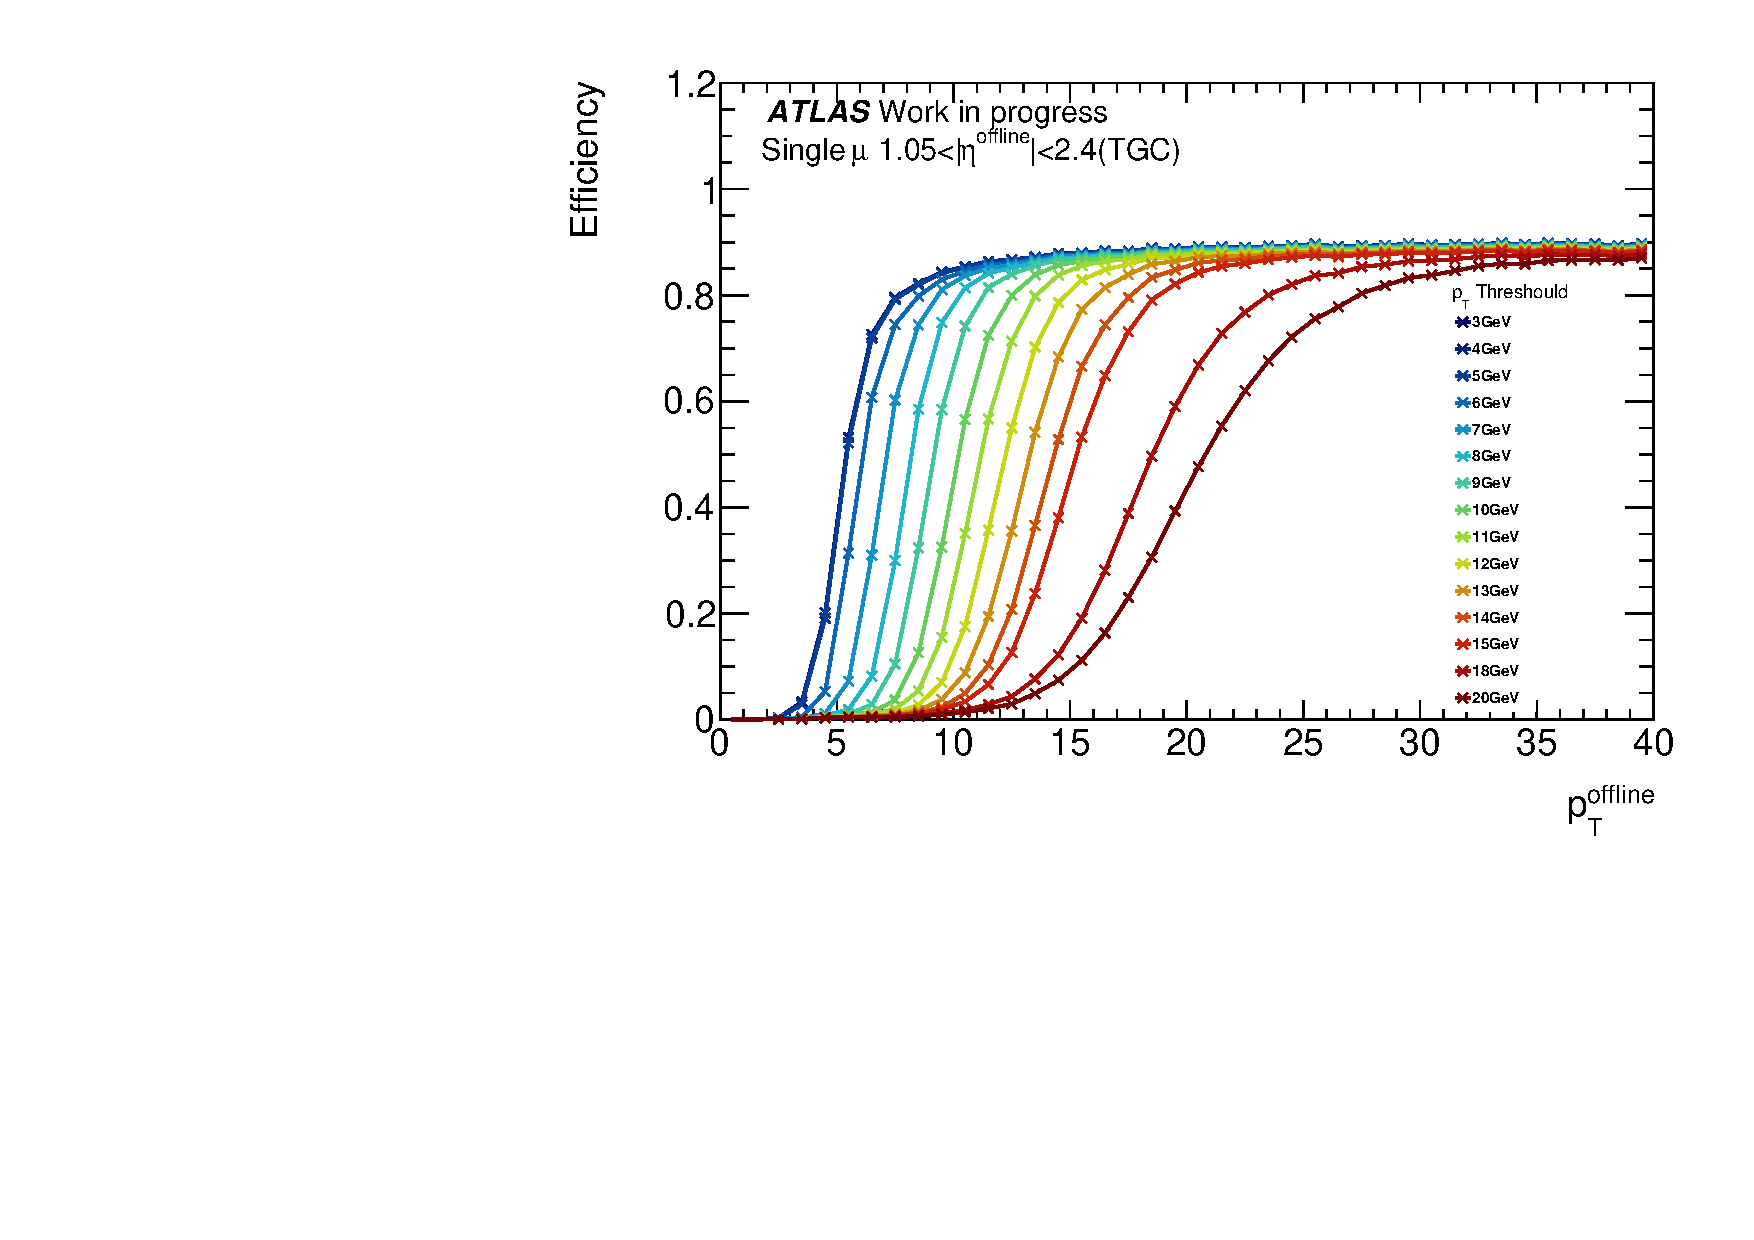
\includegraphics[clip, width=8cm]{fig/5/15_MC_MC.pdf}
        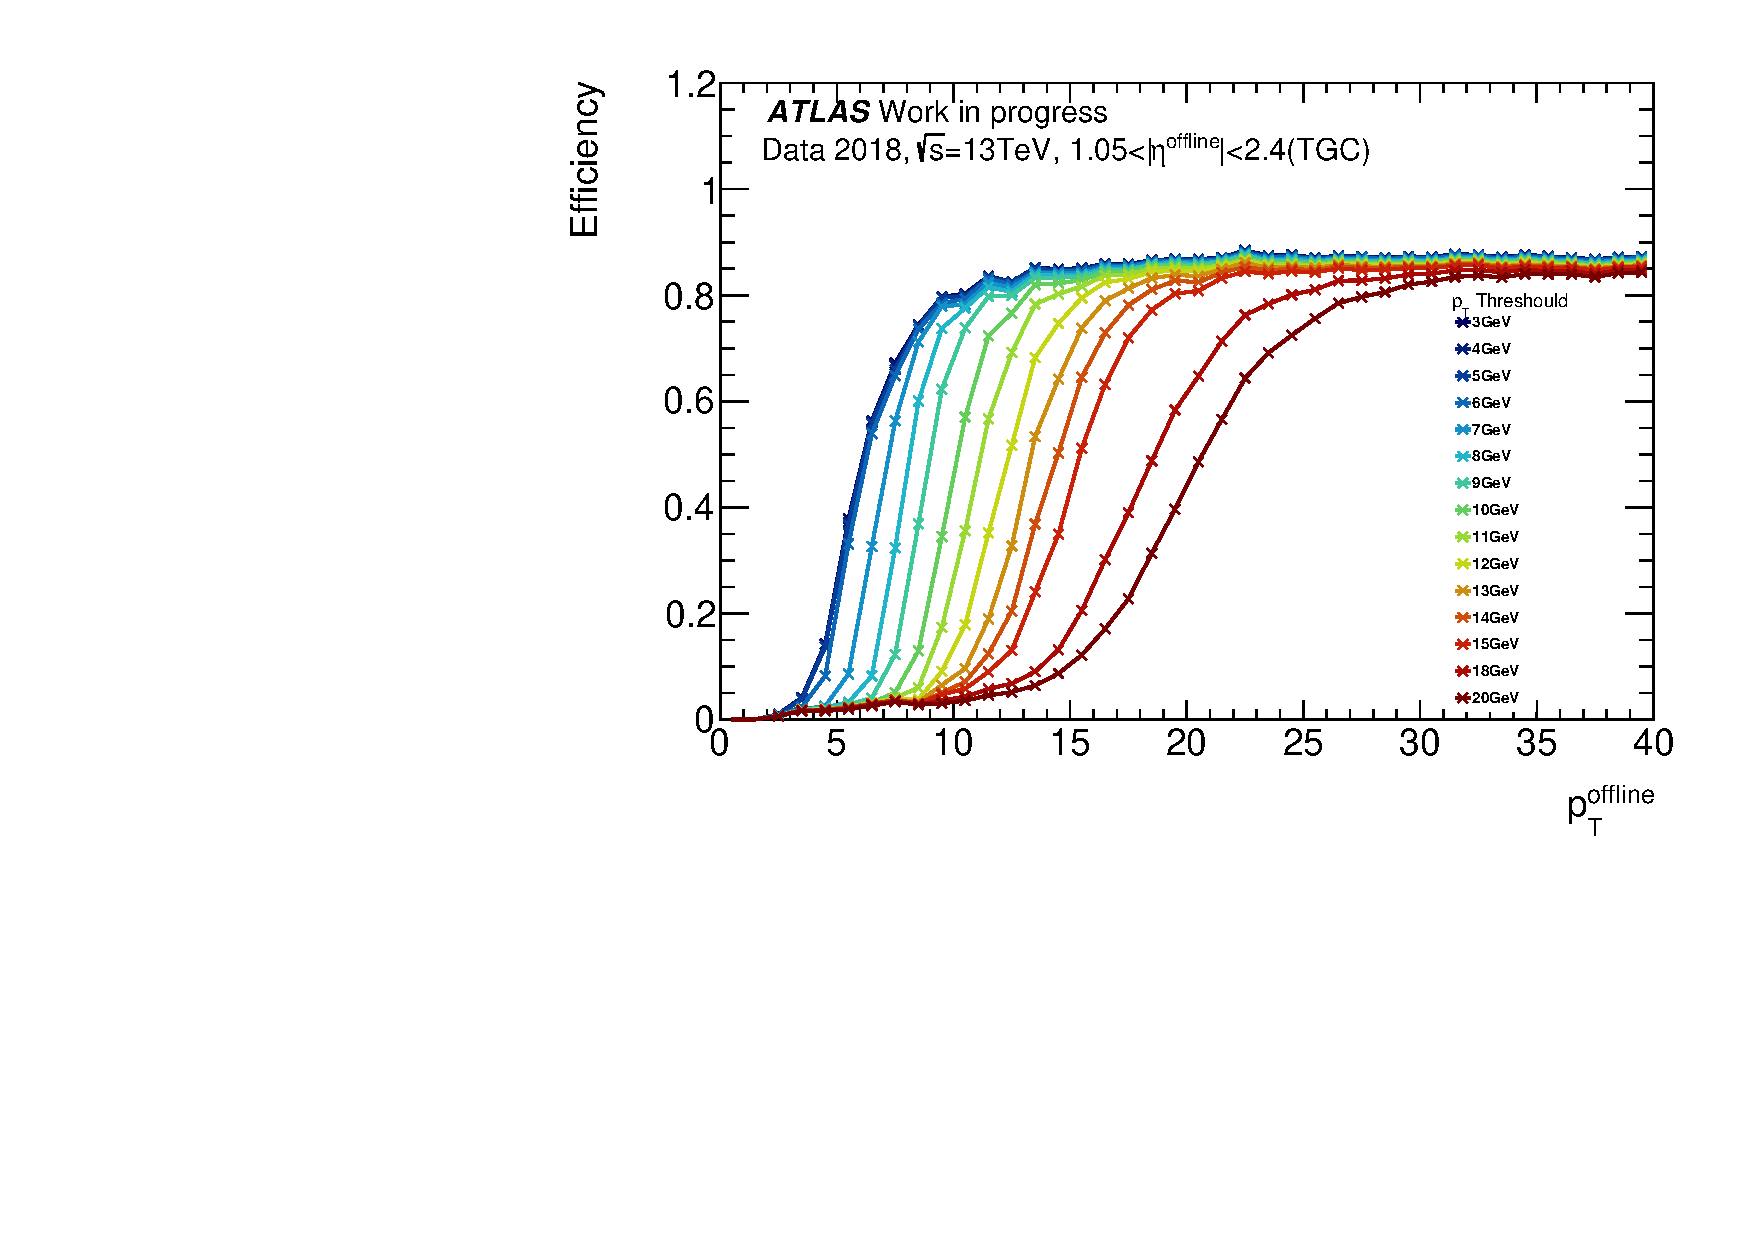
\includegraphics[clip, width=8cm]{fig/5/15_v06_Data_re.pdf}
        %\vspace{5pt}
        \subcaption{$\mathrm{CW_{Data}}$のTurn-on curve}
        \label{fig:15Eff_CW_Data}
    \end{minipage}
    \end{tabular}
    \caption{機械学習を用いて作成したCWの15段階の閾値におけるTurn-on curve。}
    \label{}
\end{figure}

\subsection{CWの最適化の効果}
TGCのチェンバーごとにミューオンの電荷別にトリガー効率を算出することでCWの最適化の効果を評価する。
あるTGCチェンバーにおける$\mathrm{CW_{Data}}$と$\mathrm{CW_{2022}}$のミューオンの電荷別に計算した$p_{\rm{T}}$閾値が14~GeVのトリガー効率を図~\ref{Eff_Chage}に示す。磁場中のミューオンは電荷によって曲がる方向が違うため、検出器アライメントのズレがある場合にはトリガー判定にミューオンの電荷依存が生じる。図~\ref{fig:v05_charge}に$\mathrm{CW_{2022}}$における電荷別に計算したTurn-on curveを示す。
$\mathrm{CW_{2022}}$は検出器のズレに対する補正を行っていないために、ミューオンの電荷別に計算したトリガー効率に大きな差が出ることが確認できる。
一方、図~\ref{fig:v06_charge}に示すように、本研究の手法で作成した$\mathrm{CW_{Data}}$は最適化されたことにより、ミューオンの電荷別に計算したTurn-on curveがほとんど一致していることが見て取れる。
\begin{figure}[htbp]
    %\centering
    \begin{tabular}{cc}
    \begin{minipage}[b]{0.45\hsize}
        %\centering
        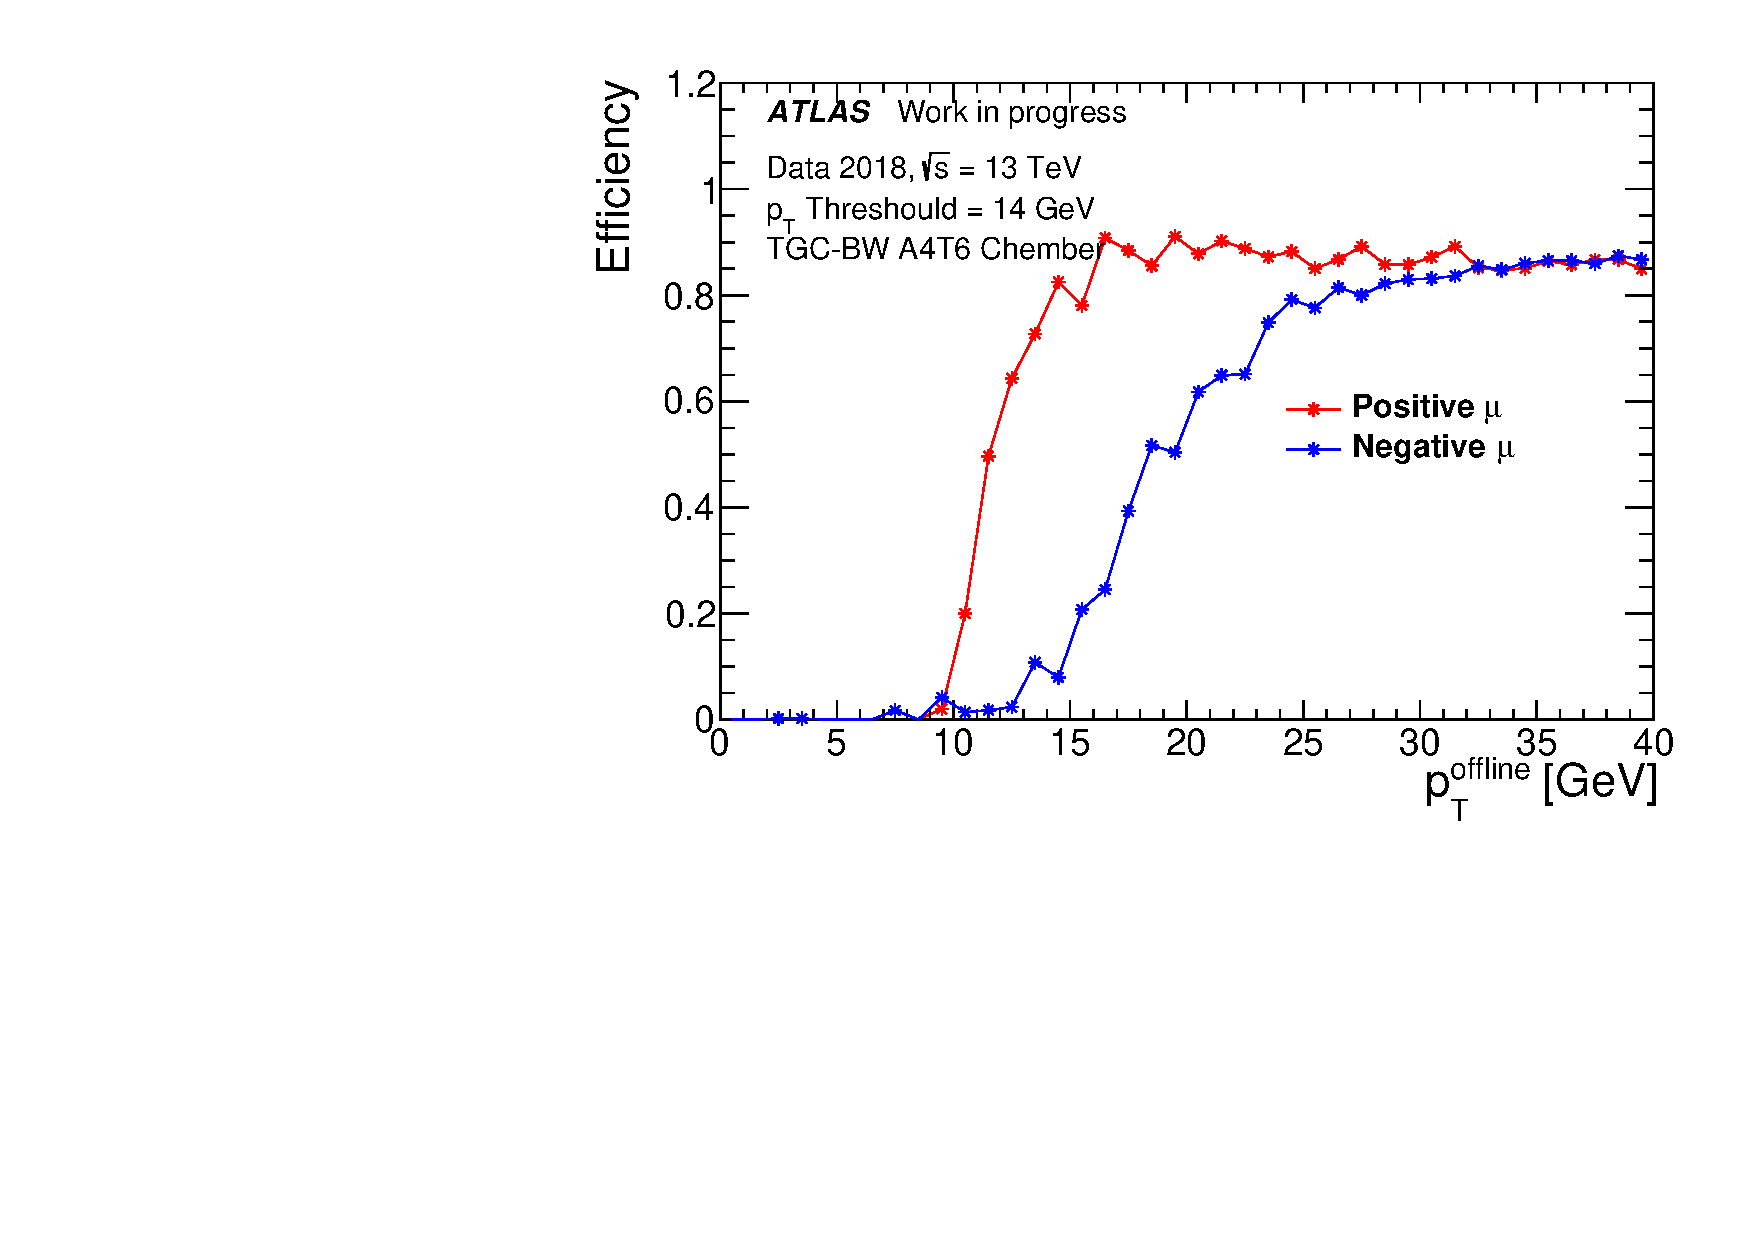
\includegraphics[clip, width=7cm]{fig/5/Eff_PNcharge_v05_phi0eta10_re.pdf}
        %\hspace{-10pt}
        \subcaption{$\mathrm{CW_{2022}}$}
        \label{fig:v05_charge}
    \end{minipage}&
    %\hfill
    \begin{minipage}[b]{0.45\hsize}
        %\centering
        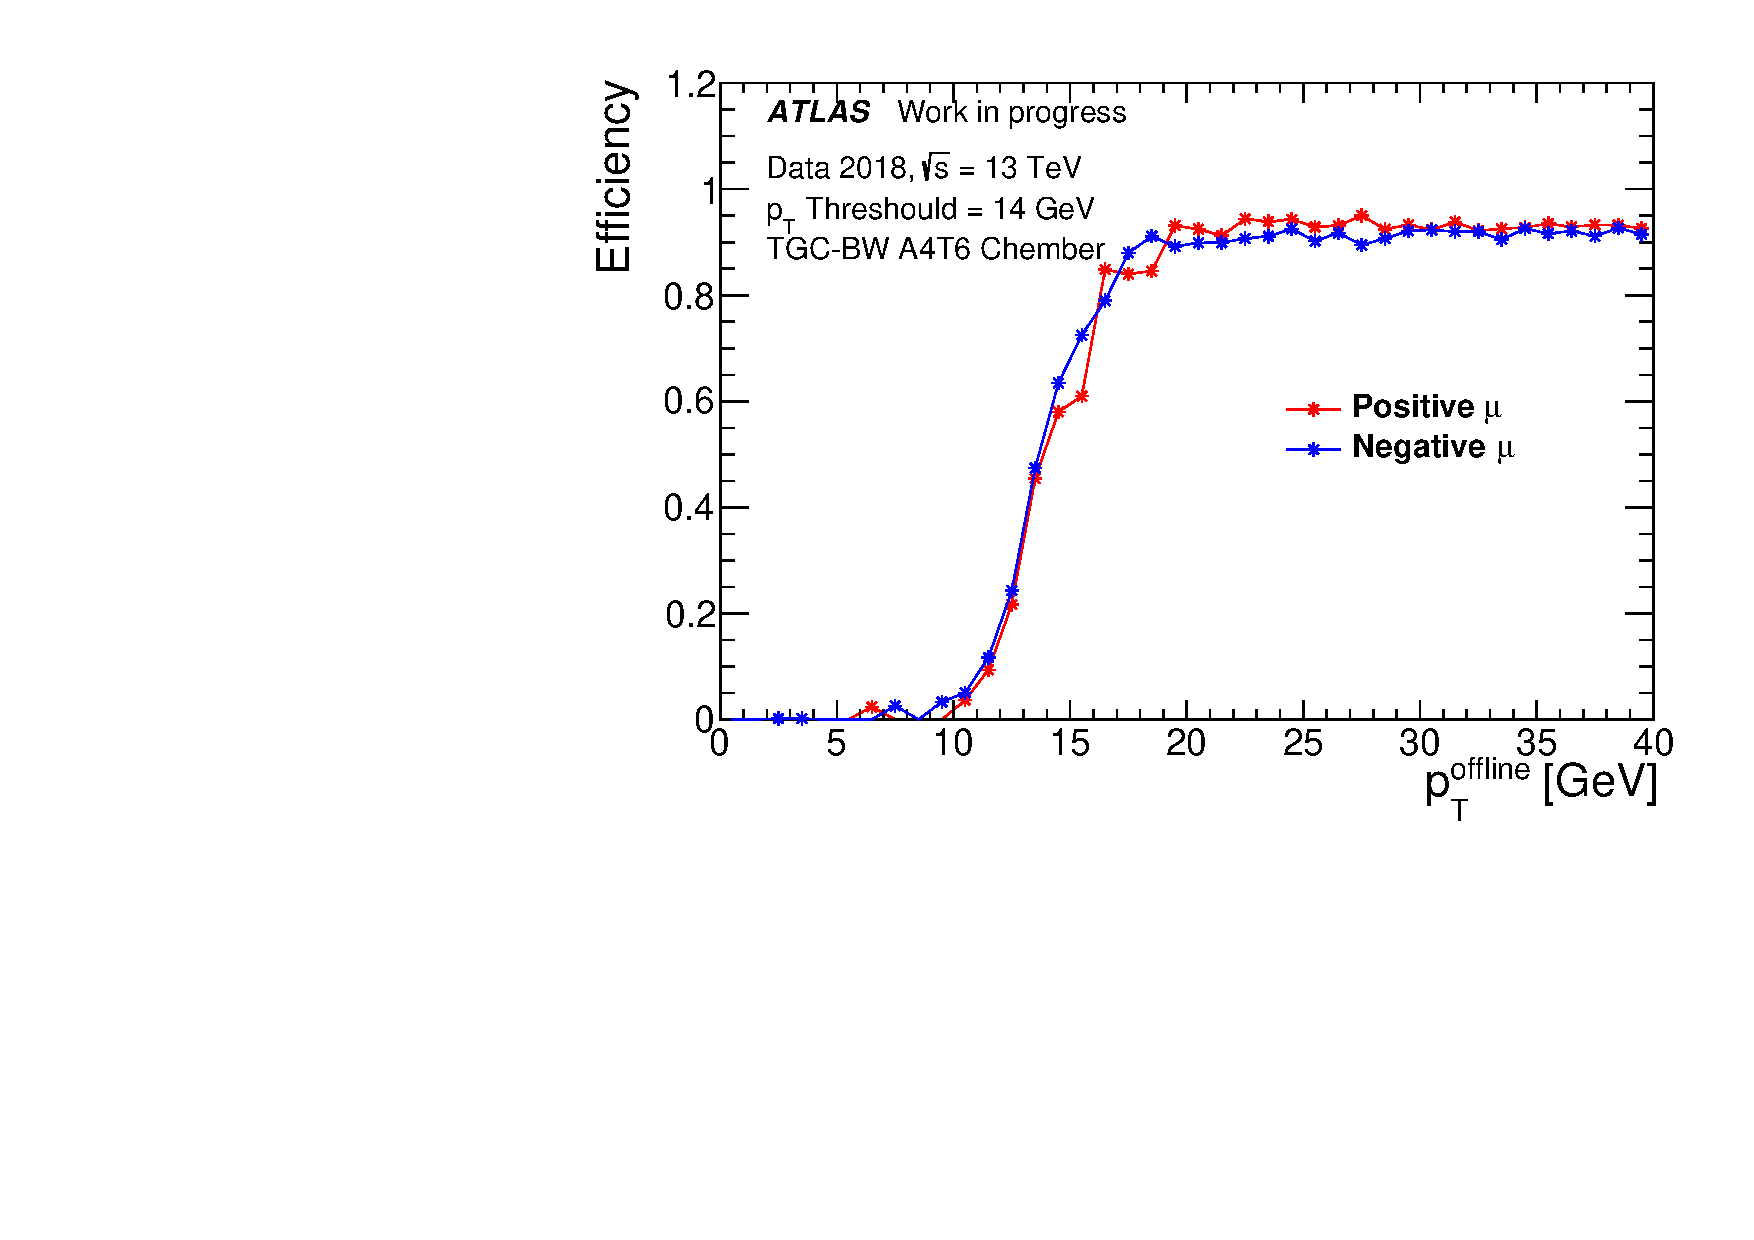
\includegraphics[clip, width=7cm]{fig/5/Eff_PNcharge_MLP_phi0eta10_re.pdf}
        %\hspace{5pt}
        \subcaption{$\mathrm{CW_{Data}}$}
        \label{fig:v06_charge}
    \end{minipage}
    \end{tabular}
    \caption{あるチェンバーにおける電荷別に計算した$p_{\rm{T}}$閾値14~GeVのTurn-on curveの比較。赤が正電荷、青が負電荷。}
    \label{Eff_Chage}
\end{figure}
さらに、この評価をTGCの全チェンバーに対して行い、正電荷と負電荷のミューオンに対するトリガー効率のEffective Thresholdの差を図~\ref{Eff_Chage_TGC}に示す。
図~\ref{fig:v05_charge_TGC}に示すように$\mathrm{CW_{2022}}$では多くのチェンバーでEffective Thresholdの差がみられるが、図~\ref{fig:v06_charge_TGC}に示すように$\mathrm{CW_{Data}}$ではCWが最適化されたことにより、Effective Thresholdの差がなくなっていることが見て取れる。これより、本研究の手法による最適化によって検出器アライメントのズレに対する補正が正しく行われていることが確認できる。

\begin{figure}[htbp]
    %\centering
    \begin{tabular}{cc}
    \begin{minipage}[b]{0.45\hsize}
        %\centering
        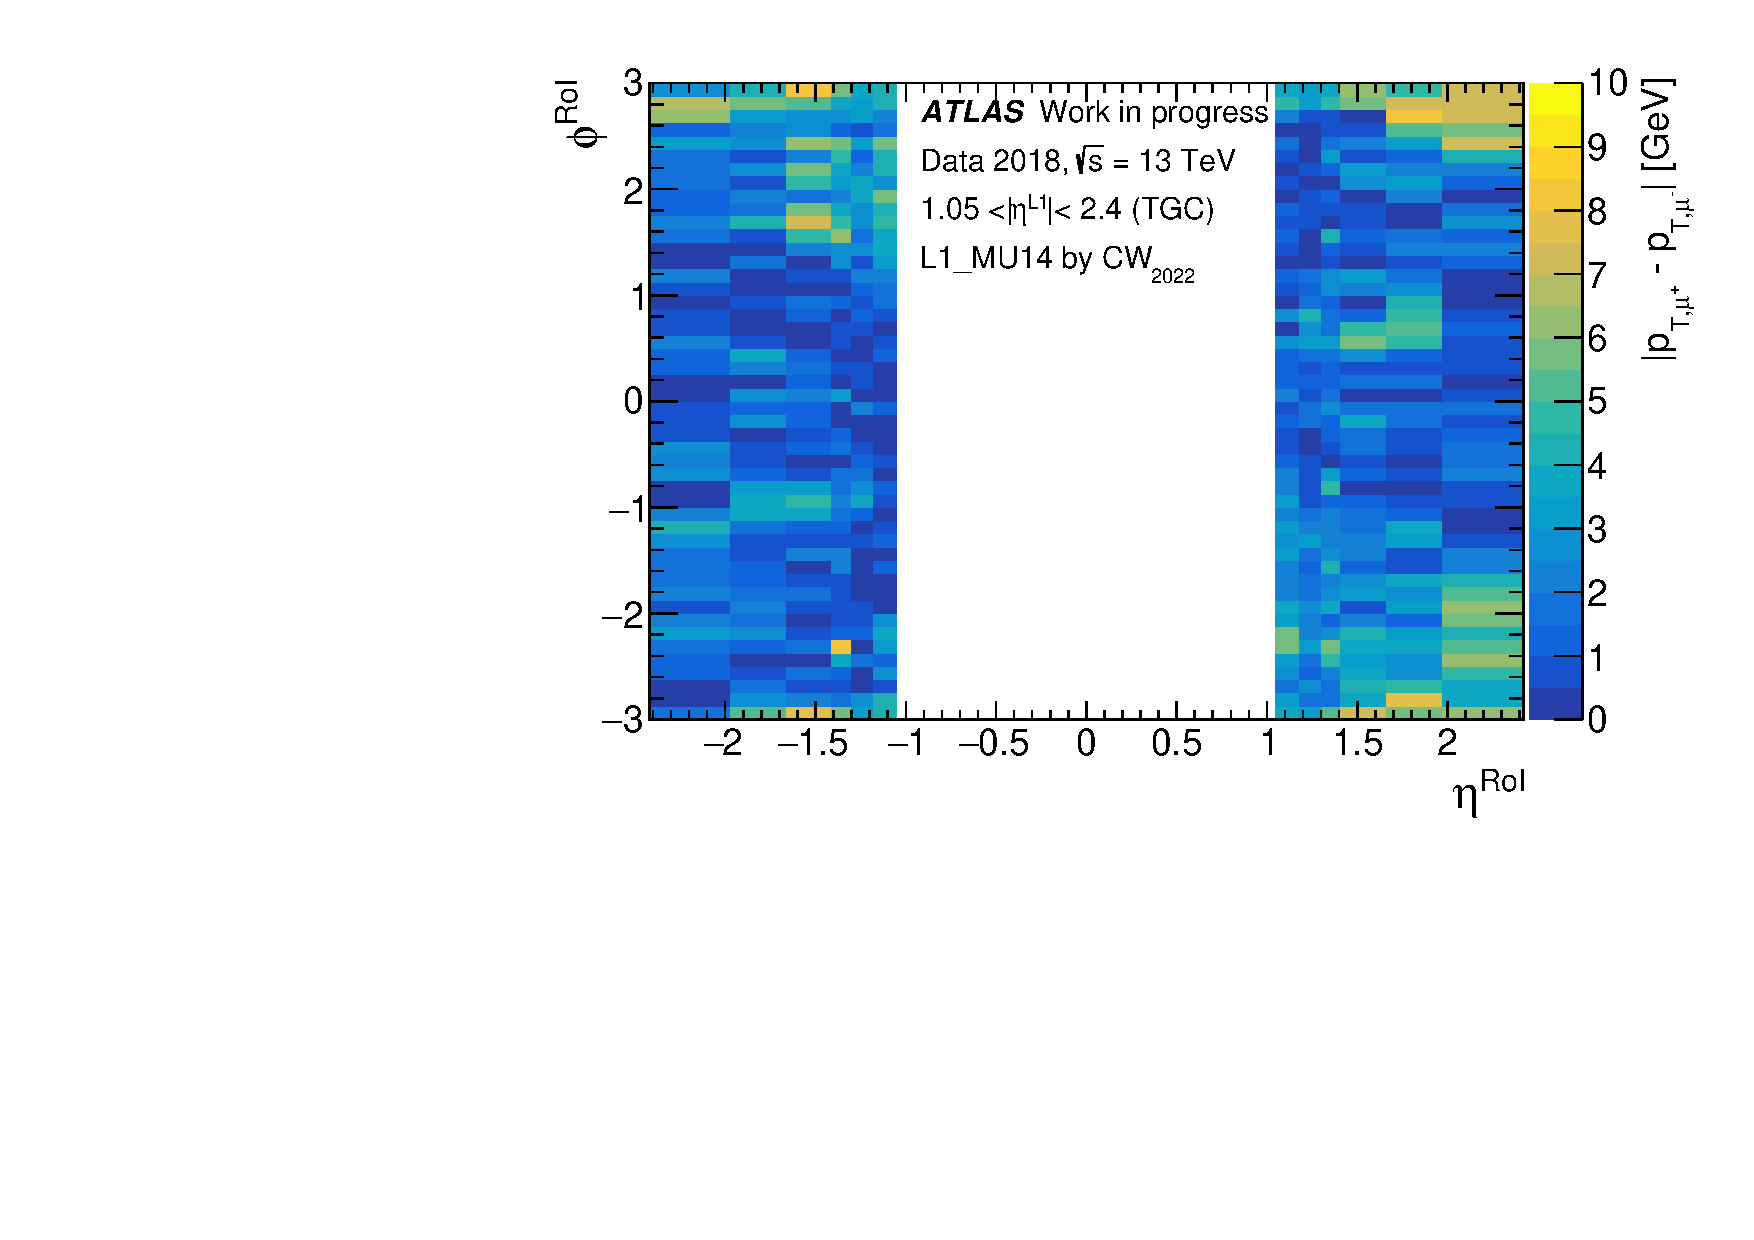
\includegraphics[clip, width=7cm]{fig/5/Eff_PNcharge_v05_re.pdf}
        \subcaption{$\mathrm{CW_{2022}}$}
        \label{fig:v05_charge_TGC}
    \end{minipage}&
    %\hfill
    \begin{minipage}[b]{0.45\hsize}
        %\centering
        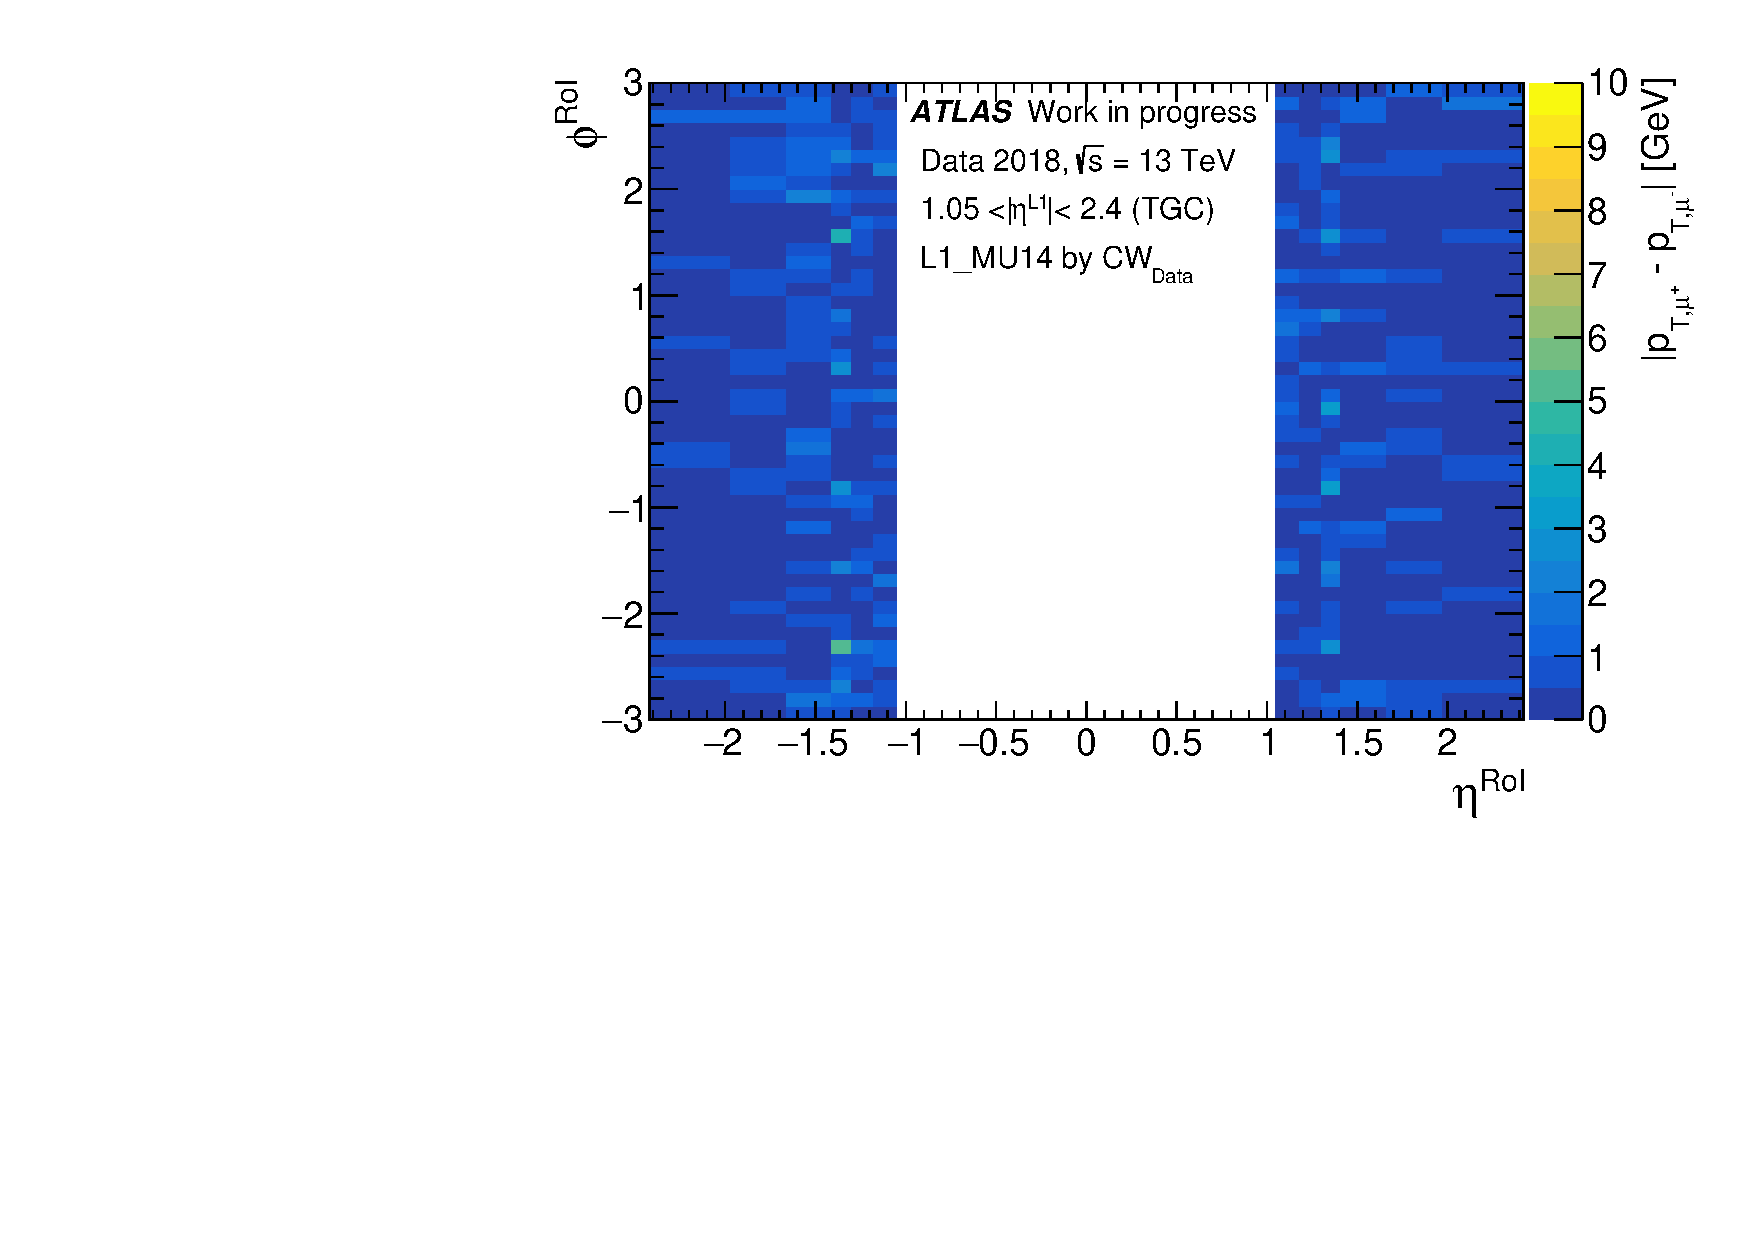
\includegraphics[clip, width=7cm]{fig/5/Eff_PNcharge_MLP_re.pdf}
        %\hspace{15pt}
        \subcaption{$\mathrm{CW_{Data}}$}
        \label{fig:v06_charge_TGC}
    \end{minipage}
    \end{tabular}
    \caption{TGCの全チェンバーにおける正電荷と負電荷のミューオンに対するトリガー効率のEffective Thresholdの差の分布。$p_{\rm{T}}$閾値14~GeVのトリガー効率を評価している。}
    \label{Eff_Chage_TGC}
\end{figure}


%まず、検出器アライメントに対応して実際にCWを補正できているかを確認する。
%8回転対象の磁場構造において、同じ磁場構造となる場所に位置するRoIのCWについて、$p_{\rm{T}}$閾値が14~GeVとなる領域の$\mathrm{CW_{Data}}$と$\mathrm{CW_{2022}}$の比較を図~\ref{fig:CWv05v07}に示す。
%図~\ref{fig:CWv05v07}に示す8個のCWは、シミュレーション上では磁場構造が同じになるため、黒枠で表される$\mathrm{CW_{2022}}$はすべて同じ形である。しかし、\ref{ズレ}節で述べたように、実際の検出器のズレによって場所によって磁場構造が異なるため、本手法で作成した$\mathrm{CW_{Data}}$ではCWに数マス分のズレが生じていることが確認できる。
%\begin{figure}[tb]
%  \centering
%  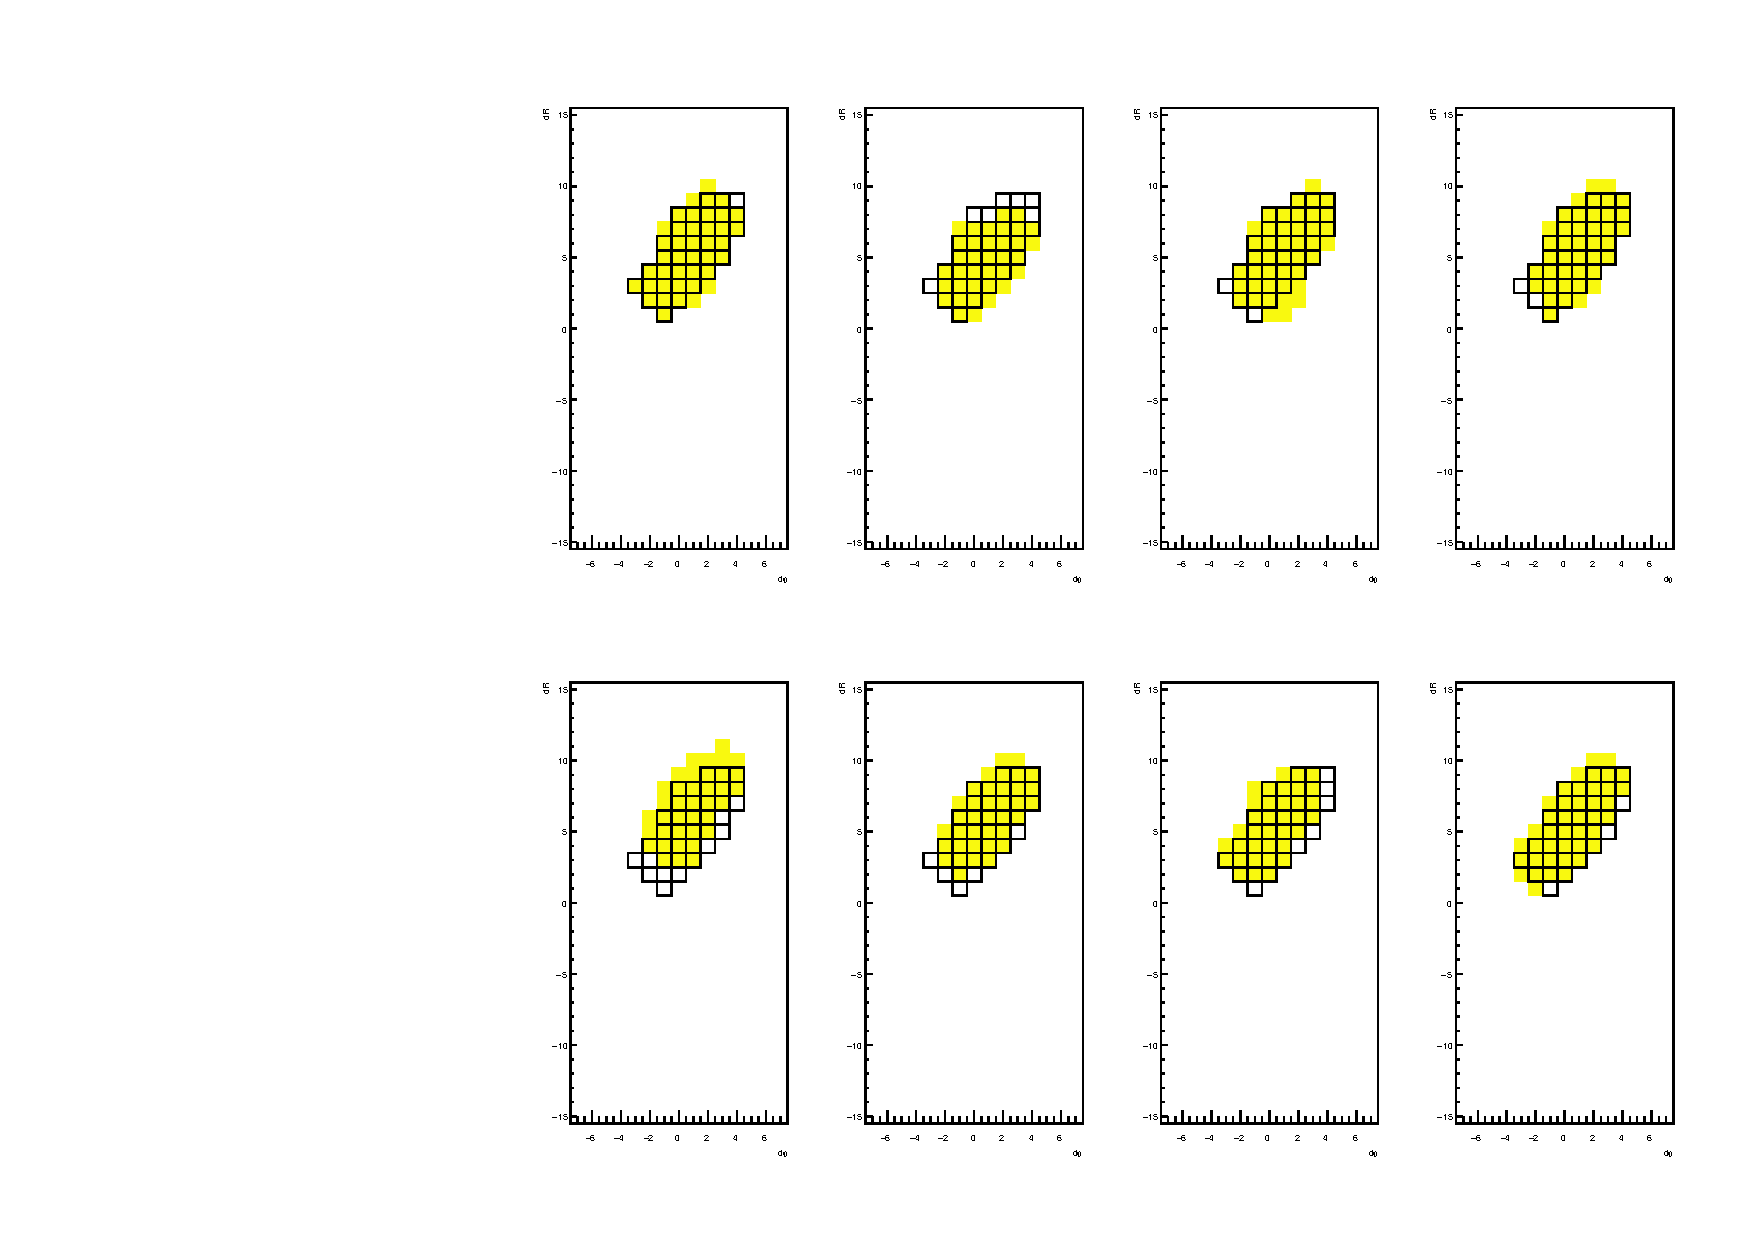
\includegraphics[clip, width=13cm]{fig/5/ALL_Aside_Endcap_phiSector_Octant1_roi58.pdf}
%  \caption{$p_{\rm{T}}$閾値が14~GeVとなる領域の比較。黄色の領域が本手法で作成した$\mathrm{CW_{Data}}$、黒枠の領域が$\mathrm{CW_{2022}}$である。}
%  \label{fig:CWv05v07}
%\end{figure}

次に、2018年Run-2データを評価に用いた時の、$\mathrm{CW_{Data}}$と$\mathrm{CW_{Simu}}$の性能の比較を行うことで、本研究の手法がトレーニングデータの違いを学習できているかを確認する。図~\ref{fig:v06v07}に$p_{\rm{T}}$閾値14~GeVにおけるTurn-on curveを比較したプロットを示す。最適化が行われた$\mathrm{CW_{Data}}$を用いたトリガーの方が、実際のデータに対してのトリガー効率が良くなっているのが見て取れる。
\begin{figure}[tb]
  \centering
  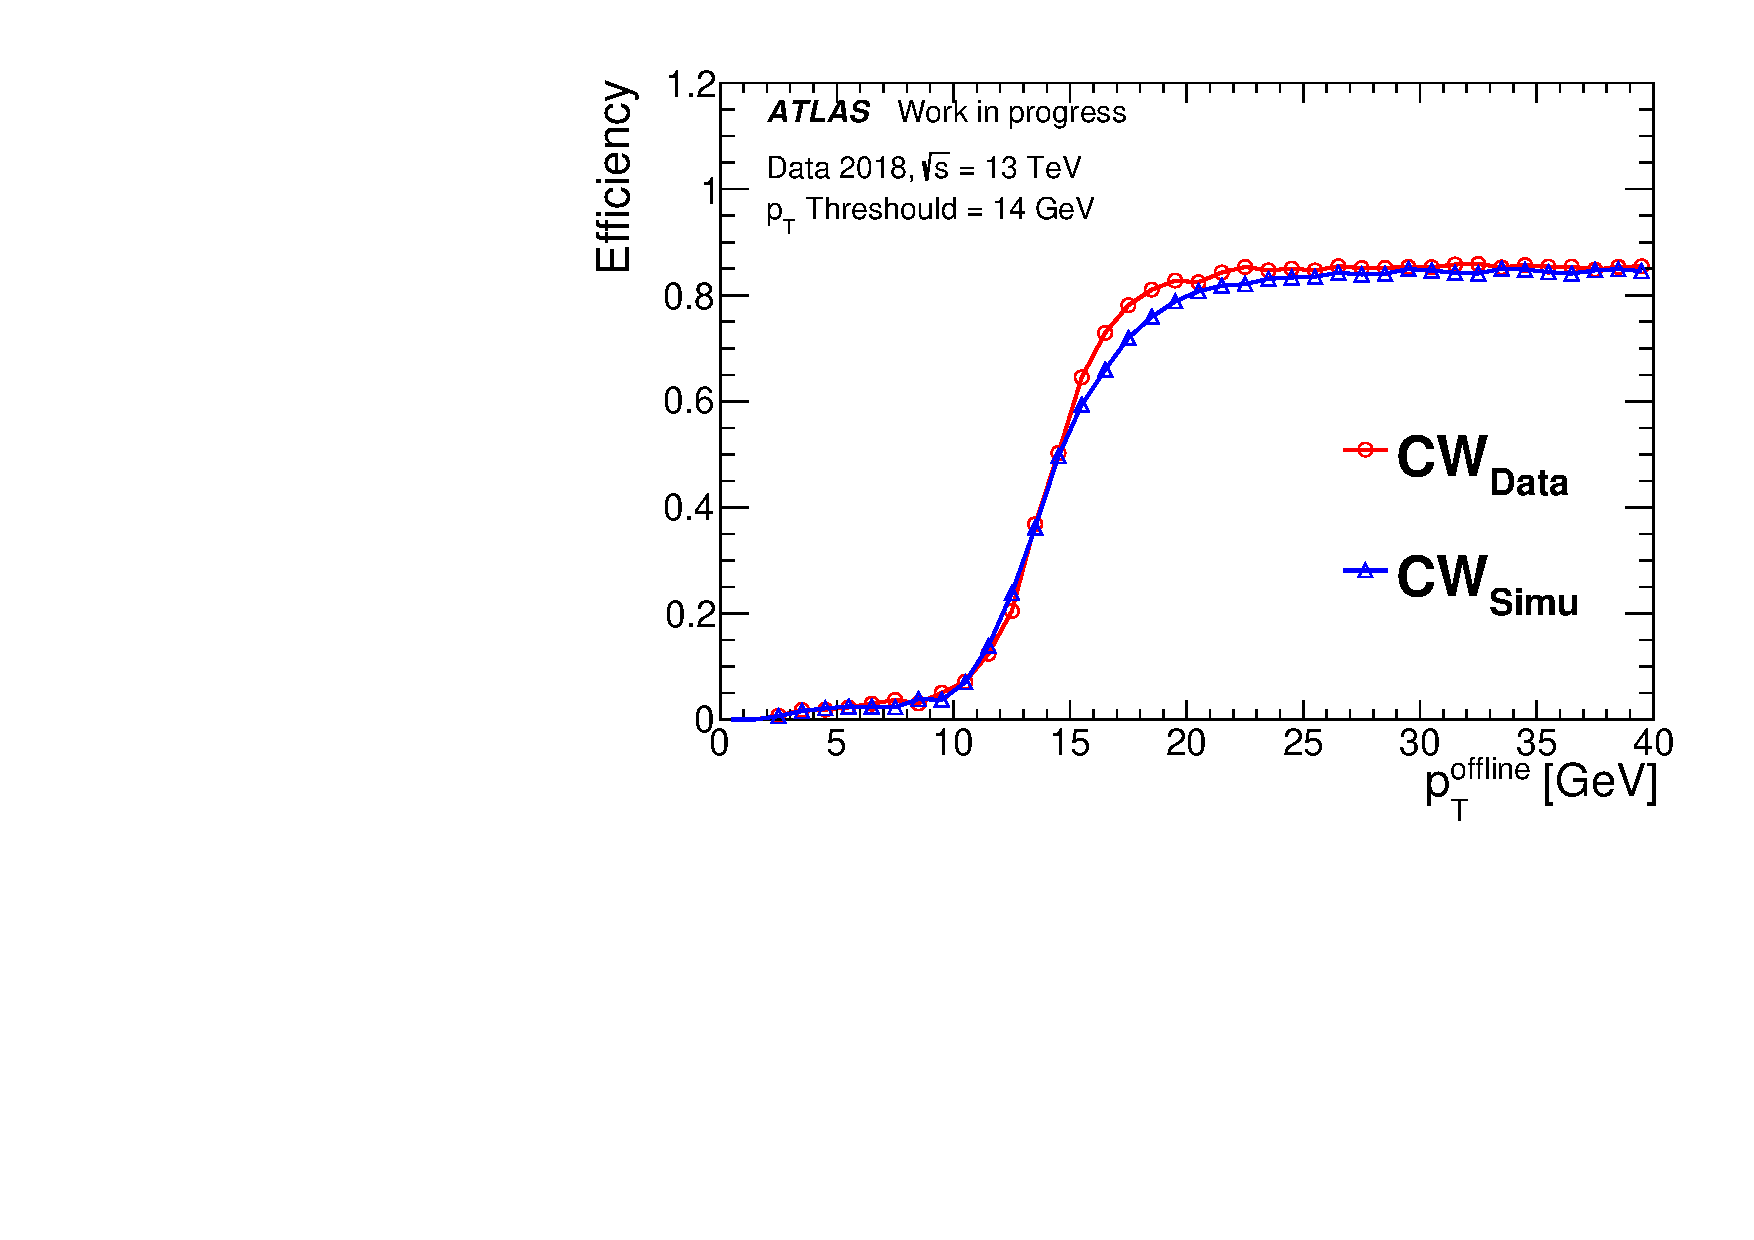
\includegraphics[clip, width=11cm]{fig/5/v06vsv07_MU14_re.pdf}
  \caption{$\mathrm{CW_{Data}}$と$\mathrm{CW_{Simu}}$のTurn-on curve。$p_{\rm{T}}$閾値14~GeVのトリガー効率の比較を行う。}
  \label{fig:v06v07}
\end{figure}

%\subsubsection{ミューオン電荷に対するトリガー性能の評価}

本研究の手法では、実際のデータを機械学習のトレーニングに用いたことで、TGC検出器の位置による磁場構造の違いや検出器のズレを自動で補正することができ、CWが最適化されたことを示している。


\subsection{現行のトリガーとのトリガー性能の比較}
次に、それぞれの15段階の$p_{\rm{T}}$閾値のトリガー性能について評価を行う。

\subsubsection{トリガー効率の評価}
まず、$\mathrm{CW_{Simu}}$と$\mathrm{CW_{2022}}$の比較と、$\mathrm{CW_{Data}}$と$\mathrm{CW_{2022}}$の比較を行う。それぞれの評価には、シングルミューオンのシミュレーションデータと2018年Run-2のデータを評価に用いる。
ここでは、式~\ref{equ:Eff}で示したトリガー効率$\epsilon$を用いて比較を行う。

図~\ref{fig:v05v07}には$p_{\rm{T}}$閾値が14~GeVの時の、$\mathrm{CW_{2022}}$と$\mathrm{CW_{Simu}}$のTurn-on curveの比較を示し、図~\ref{fig:v05v06}には$p_{\rm{T}}$閾値が14~GeVの時の、$\mathrm{CW_{Data}}$を$\mathrm{CW_{2022}}$のTurn-on curveの比較を示す。
2022年度Run-3で使用されている$\mathrm{CW_{2022}}$に比べて、本研究の手法ので作成したCWの方がTurn-on curveの立ち上がりが鋭くなっており、トリガー性能が良くなっていることが見て取れる。
このとき、$\mathrm{CW_{2022}}$はトリガー効率が85.4$\%$であったのに対し、$\mathrm{CW_{Data}}$ではトリガー効率が86.7$\%$となったことから、約1$\%$の向上が確認できた。
また、図~\ref{fig:v05v07_1_9_Simu}と図~\ref{fig:v05v06_1_9_Data}に他の$p_{\rm{T}}$閾値における比較を示す。
15段階の閾値において、本研究の手法によって作成された2種類のCWは、2022年度Run-3において使用された$\mathrm{CW_{2022}}$と同様に鋭く立ち上がっていることが見て取れる。
\begin{figure}
    %\centering
    \begin{tabular}{cc}
    \centering
    \begin{minipage}[b]{0.45\hsize}%
        \centering
        \hspace*{-1.5cm}
        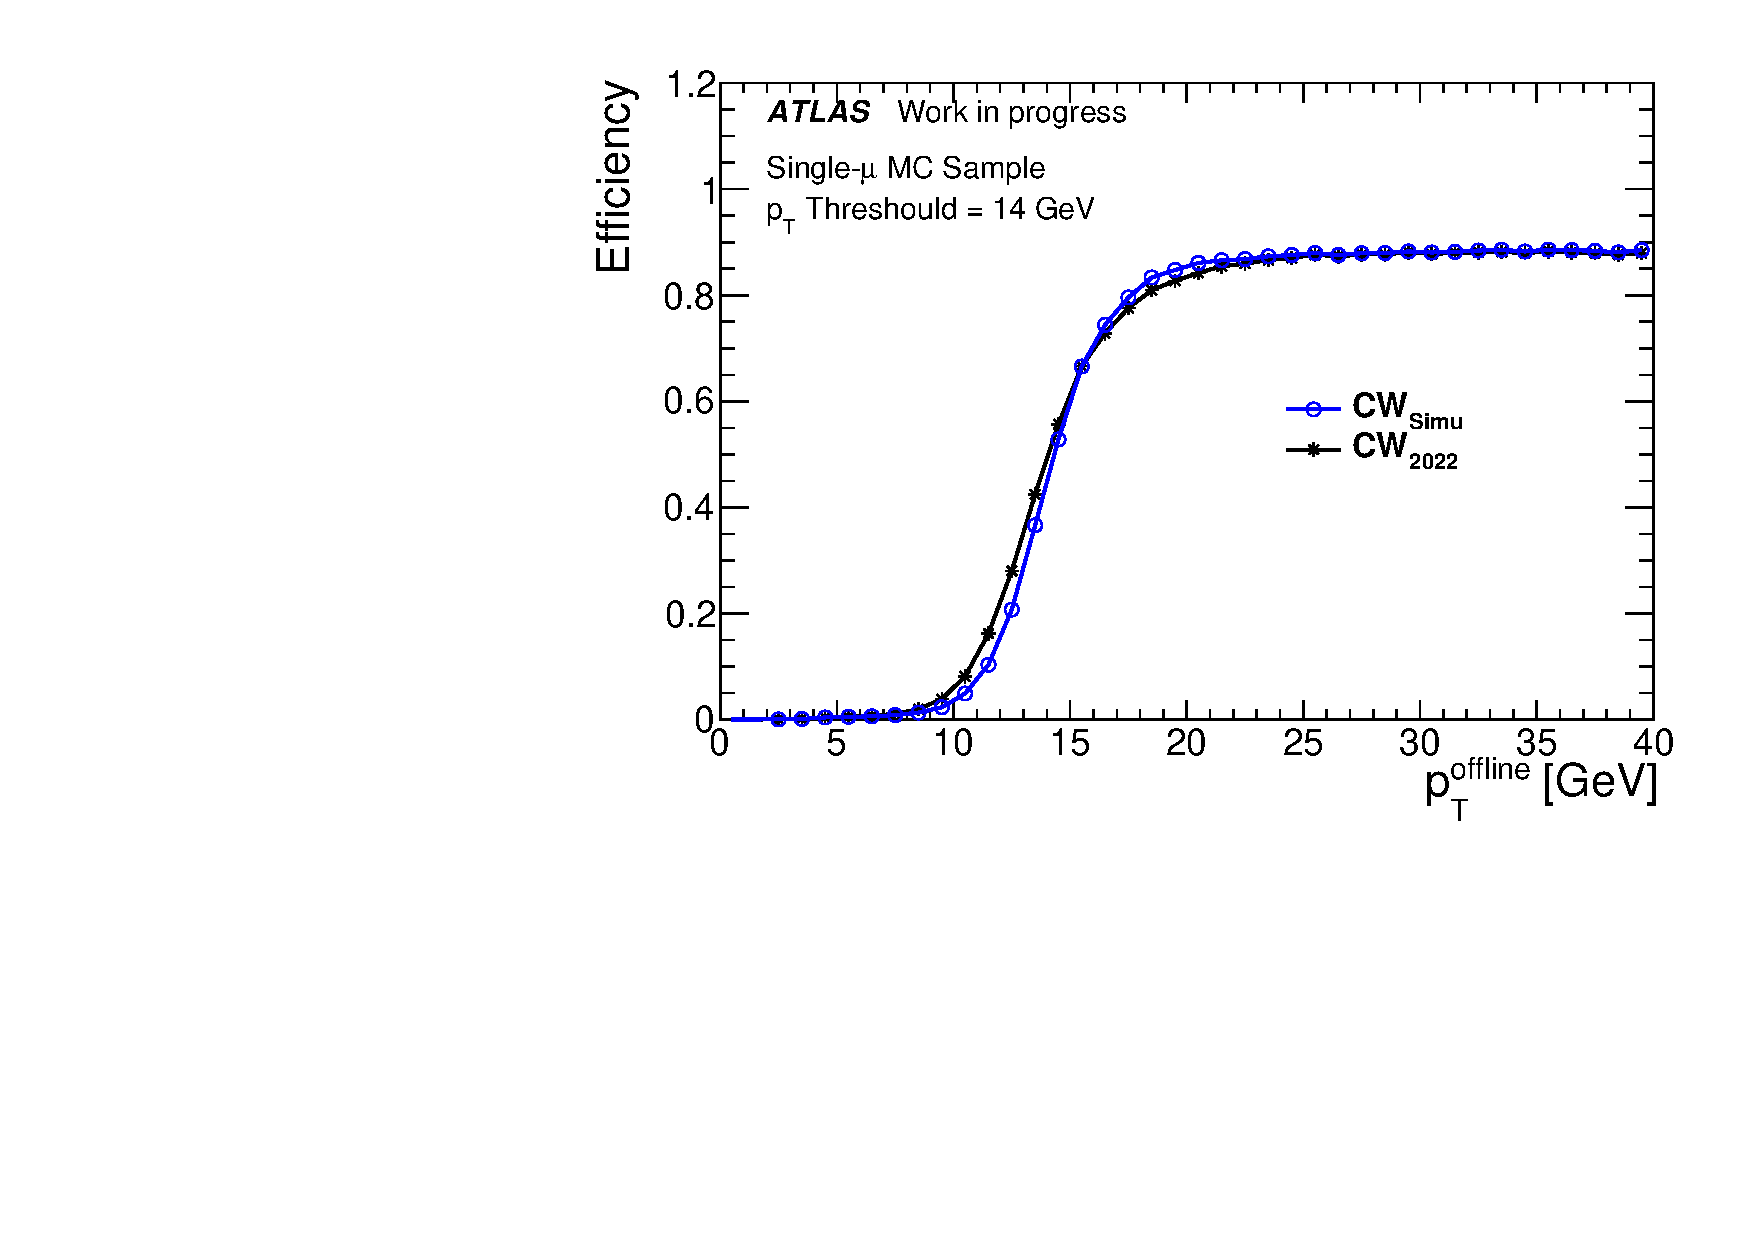
\includegraphics[clip, width=8cm]{fig/5/v05vsv07_MU14_re2.pdf}
        %\vspace{5pt}
        \subcaption{$\mathrm{CW_{Simu}}$と$\mathrm{CW_{2022}}$の比較。}
        \label{fig:v05v07}
    \end{minipage}%
    %\hfill
    \begin{minipage}[b]{0.7\hsize}%
        \centering
        \hspace*{-0.75cm}
        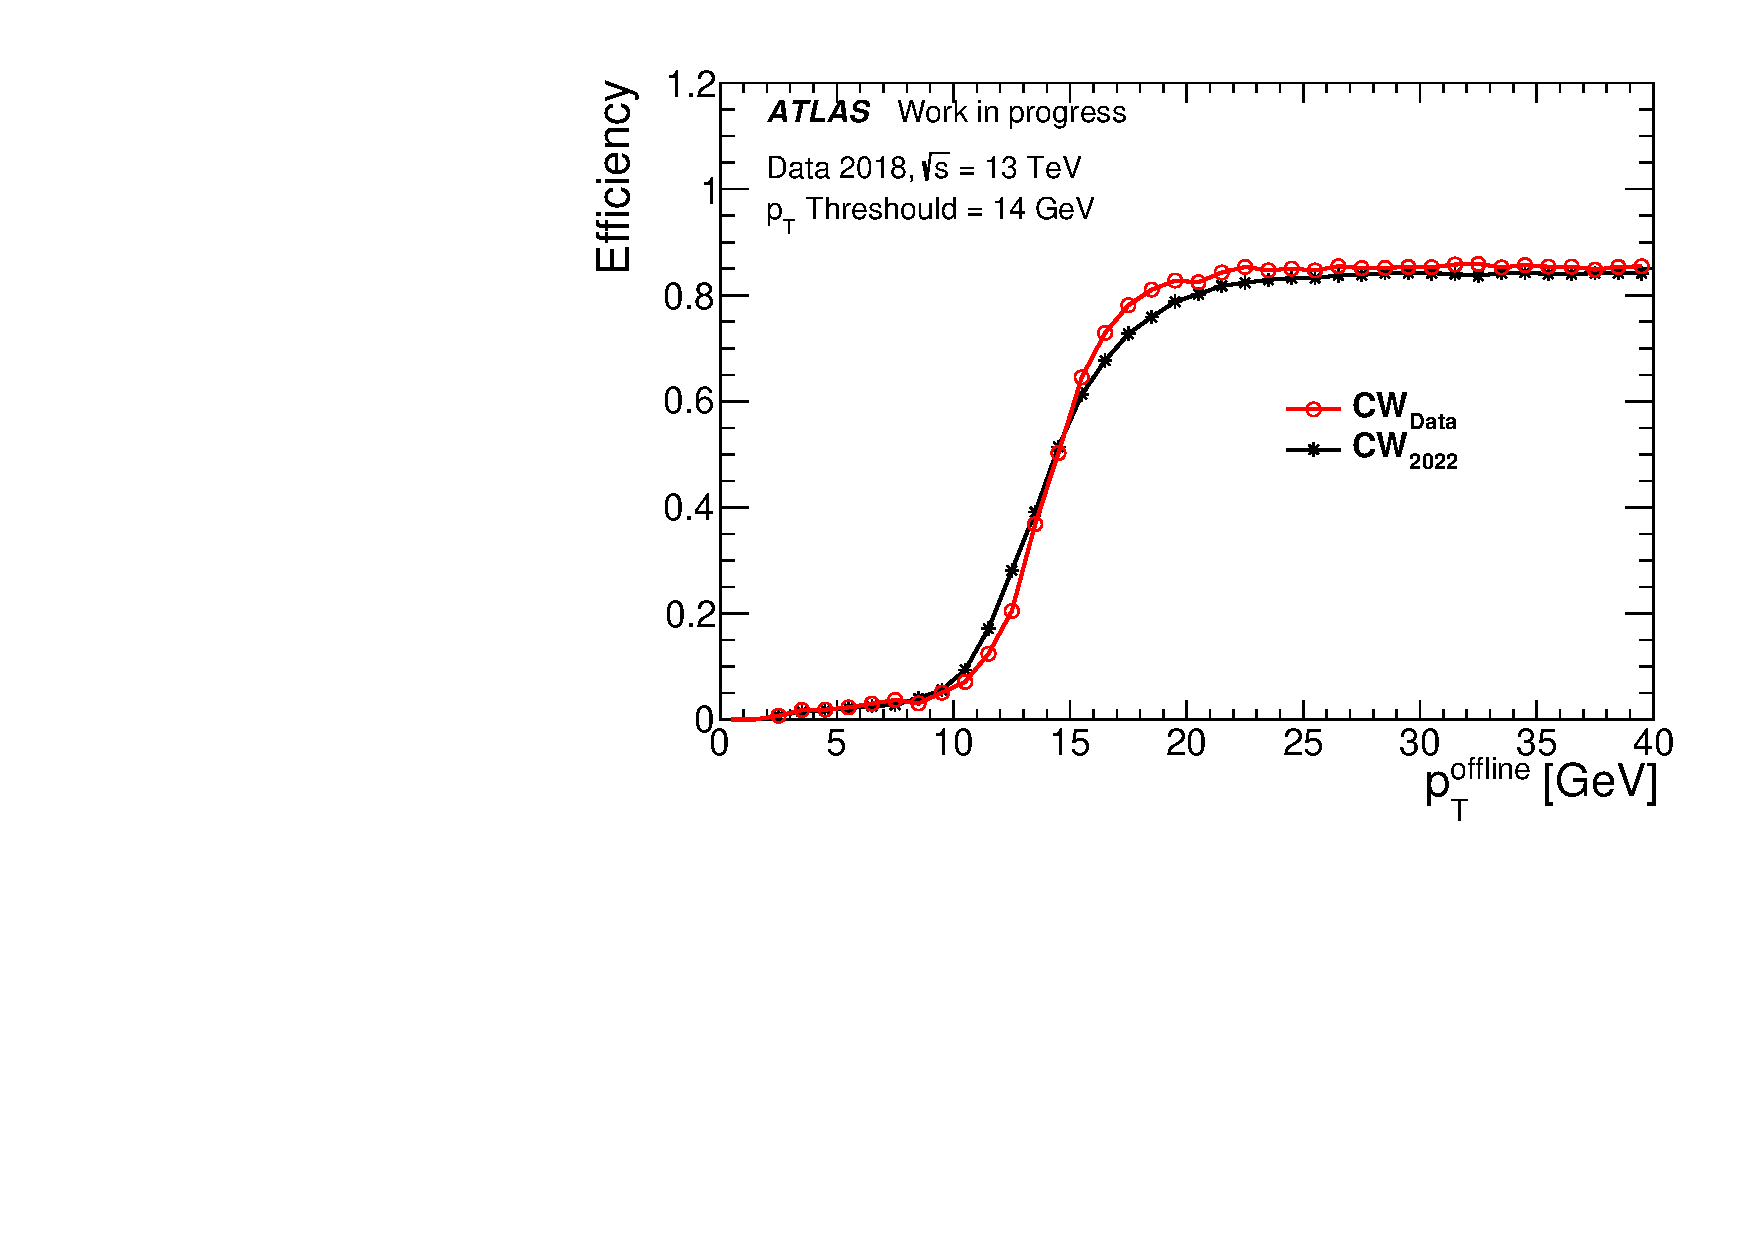
\includegraphics[clip, width=8cm]{fig/5/v05vsv06_MU14_re.pdf}
        %\vspace{5pt}
        \subcaption{$\mathrm{CW_{Data}}$と$\mathrm{CW_{2022}}$の比較。}
        \label{fig:v05v06}
    \end{minipage}%
    \end{tabular}
    \caption{$p_{\rm{T}}$閾値14~GeVにおけるTurn-on curveの比較。}
    \label{fig:v05v07v06}
\end{figure}

\begin{figure}[p]
  \centering
  %\rule{8cm}{6cm}
  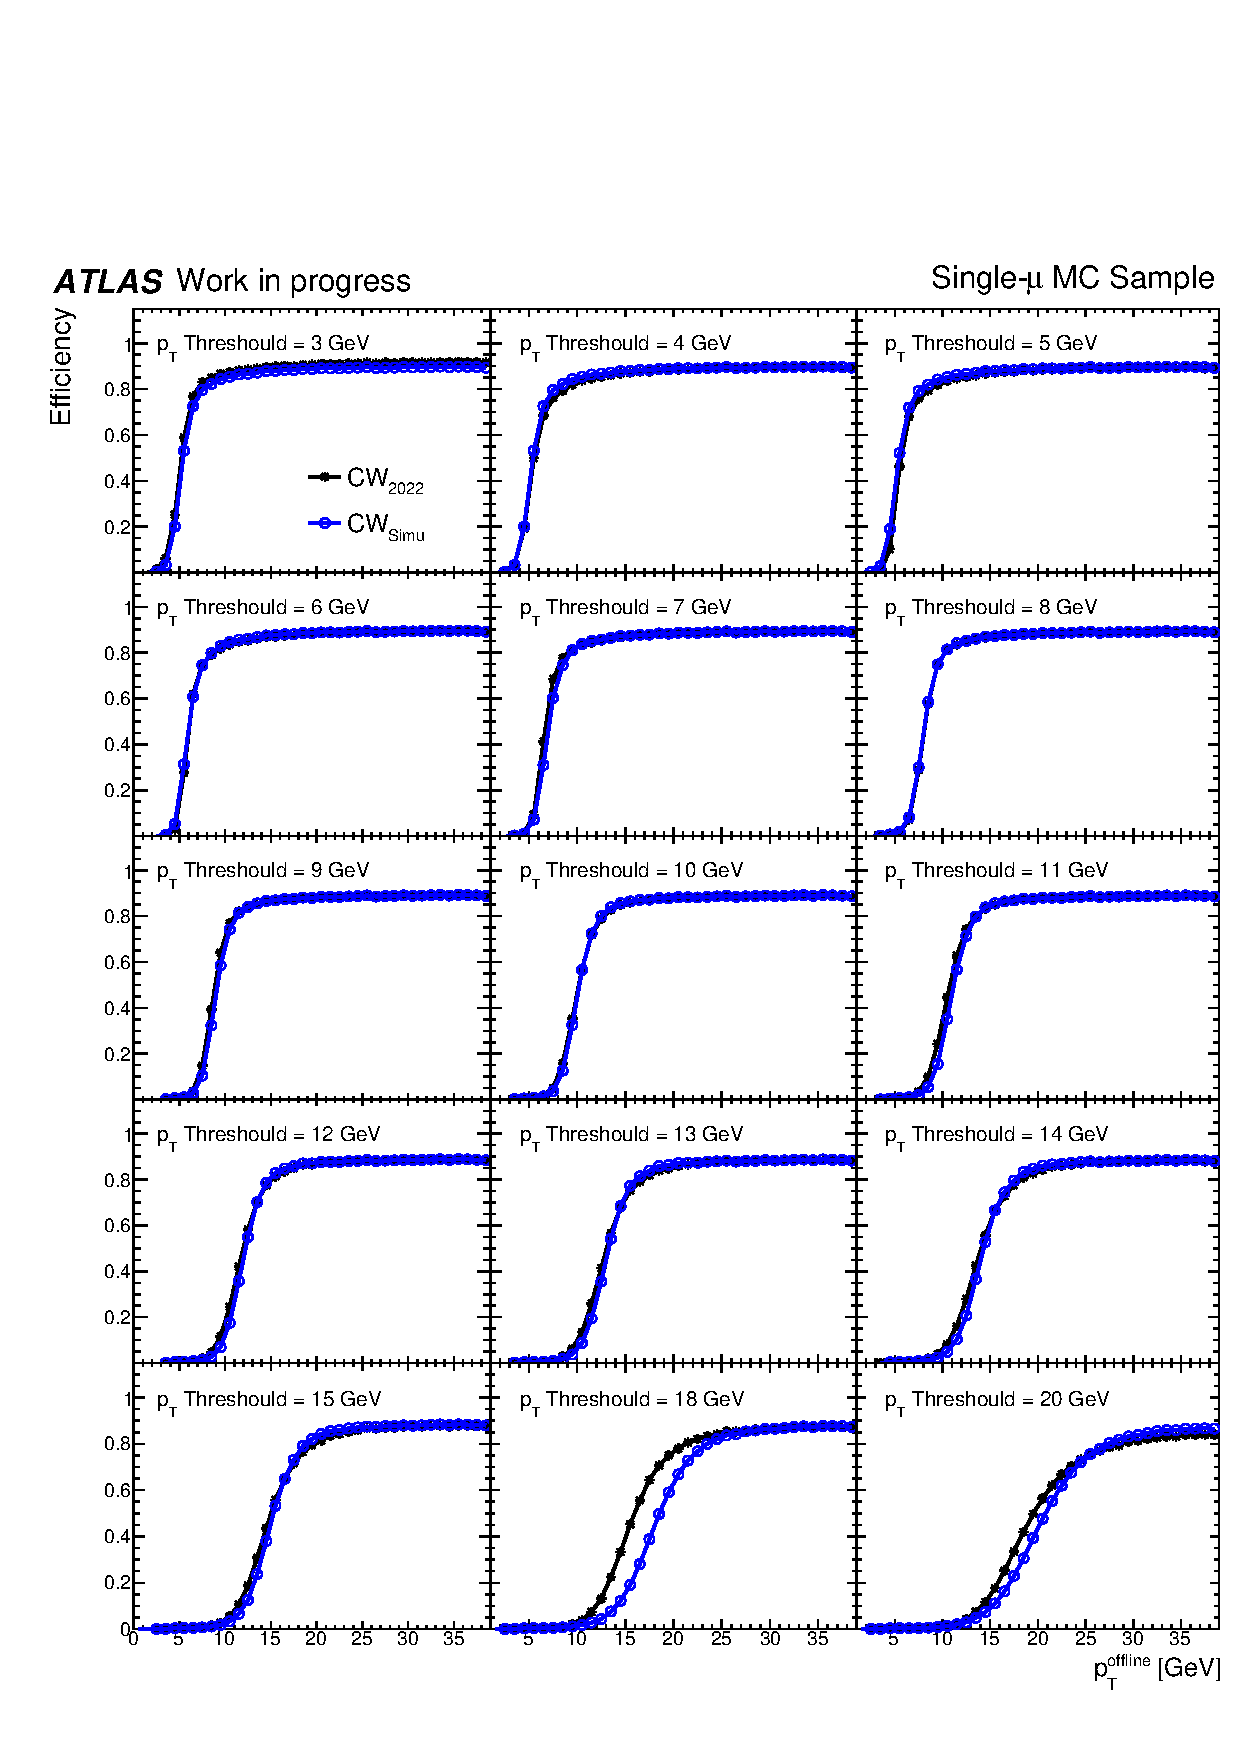
\includegraphics[clip, width=14cm]{fig/5/c2_re.pdf}
  \caption{$p_{\rm{T}}$閾値3~GeV$\sim$20~GeVにおける$\mathrm{CW_{Simu}}$と$\mathrm{CW_{2022}}$のTurn-on curveの比較。評価にはシングルミューオンのシミュレーションデータを使用した。}
  \label{fig:v05v07_1_9_Simu}
\end{figure}


%\begin{figure}[htb]
%  \centering
%  %\rule{8cm}{6cm}
%  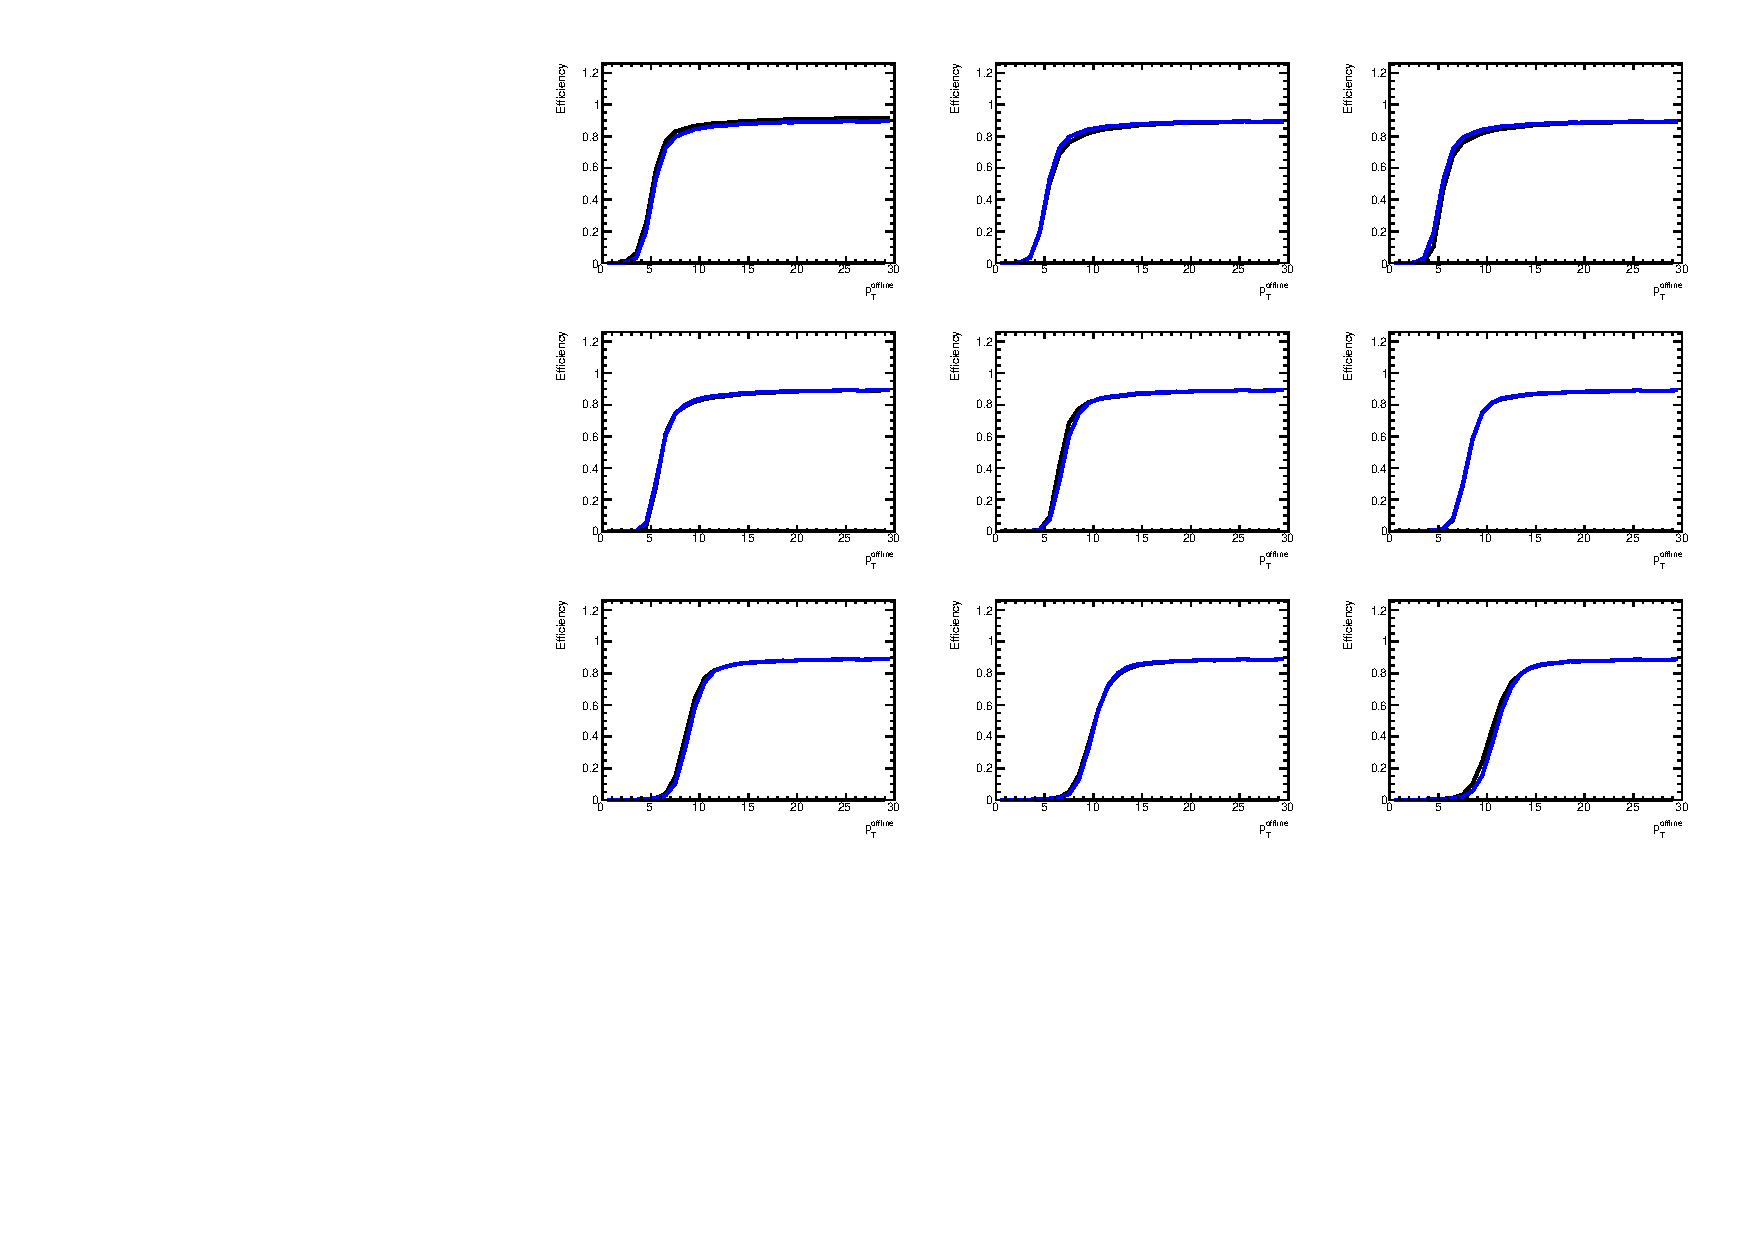
\includegraphics[clip, width=10cm]{fig/5/v05v07_1_9.pdf}
%  \caption{$p_{\rm{T}}$閾値3~GeV$\sim$9~GeVにおける$\mathrm{CW_{Simu}}$と$\mathrm{CW_{2022}}$のTurn-on curveの比較。評価にはシングルミューオンのシミュレーションデータを使用した。}
%  \label{fig:v05v07_1_9_Simu}
%\end{figure}

%\begin{figure}[htb]
%  \centering
%  %\rule{8cm}{6cm}
%  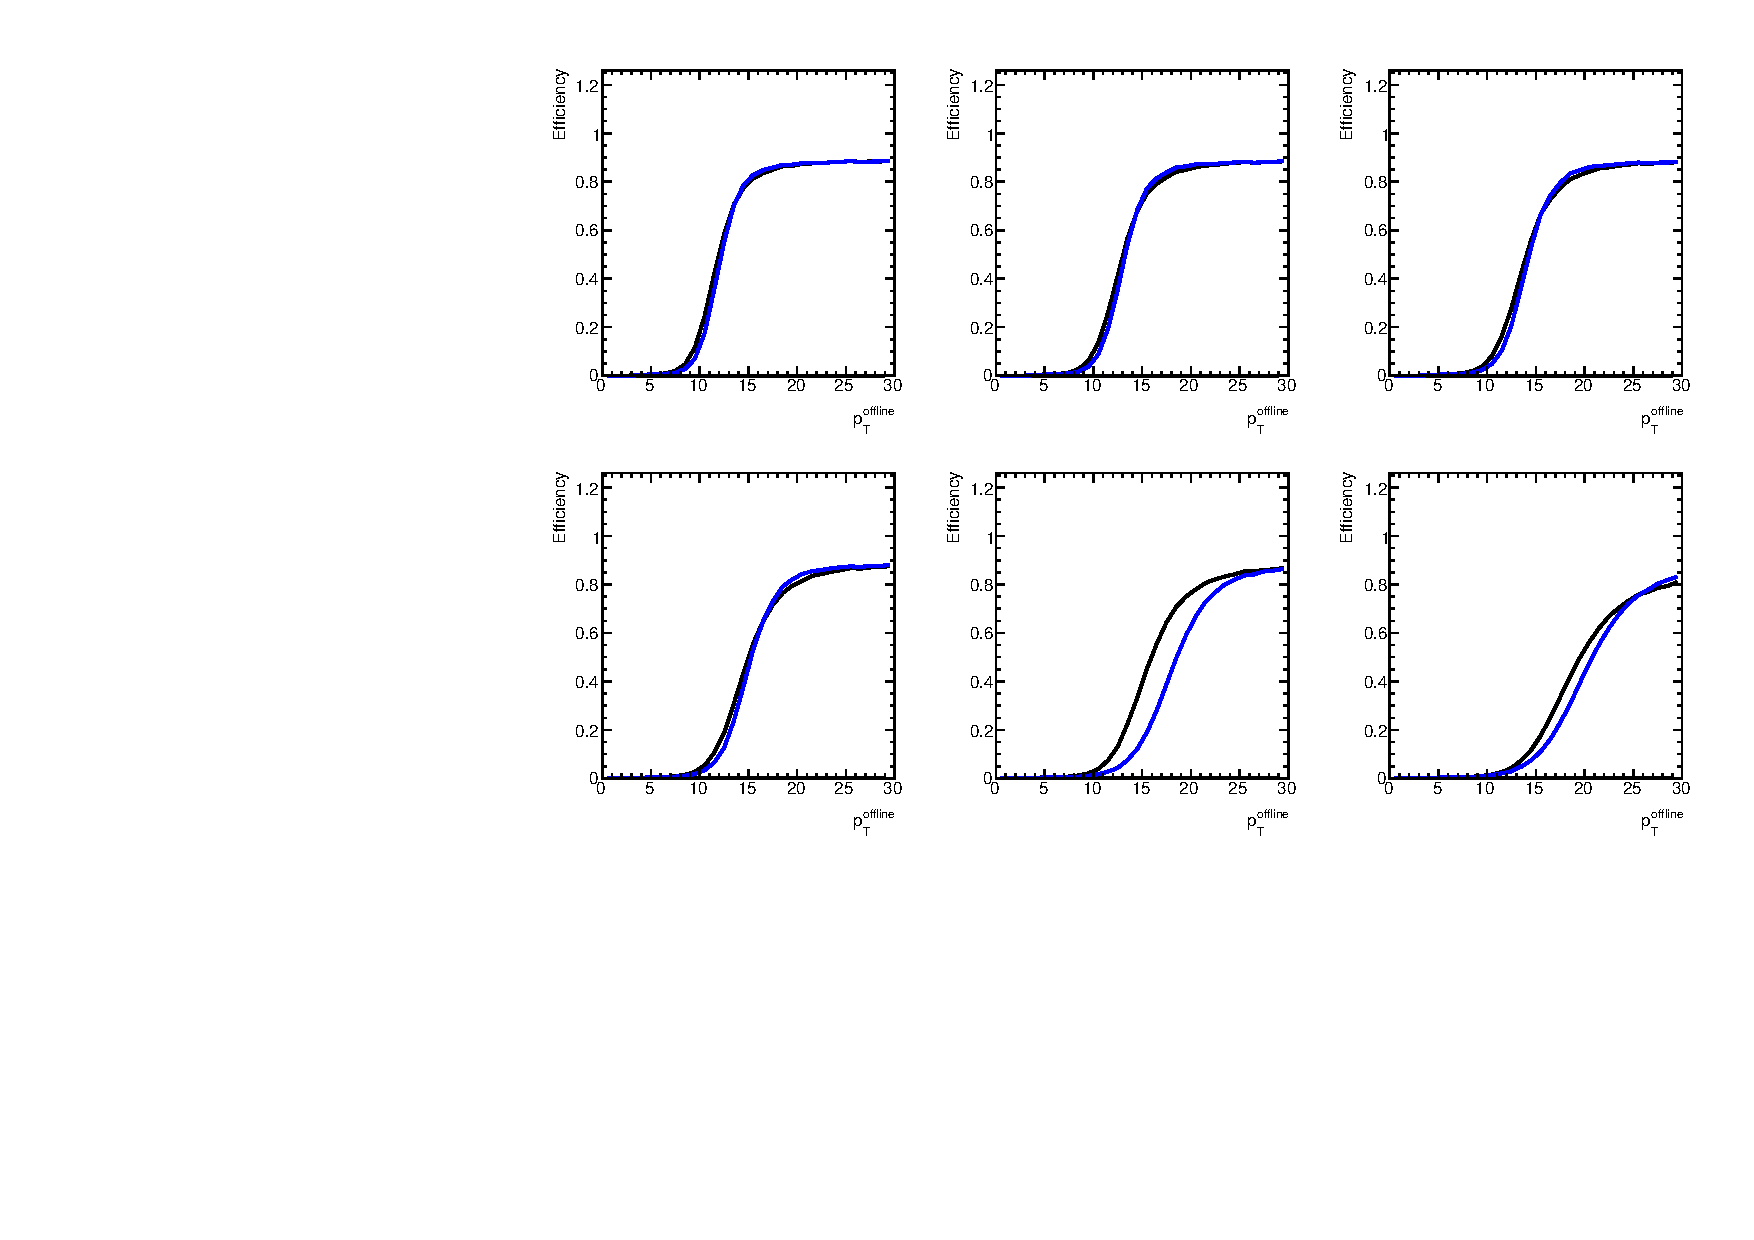
\includegraphics[clip, width=10cm]{fig/5/v05v07_10_15.pdf}
%  \caption{$p_{\rm{T}}$閾値10~GeV$\sim$20~GeVにおける$\mathrm{CW_{Simu}}$と$\mathrm{CW_{2022}}$のTurn-on curveの比較。評価にはシングルミューオンのシミュレーションデータを使用した。}
%  \label{fig:v05v07_12_20_Simu}
%\end{figure}

\begin{figure}[p]
  \centering
  %\rule{8cm}{6cm}
  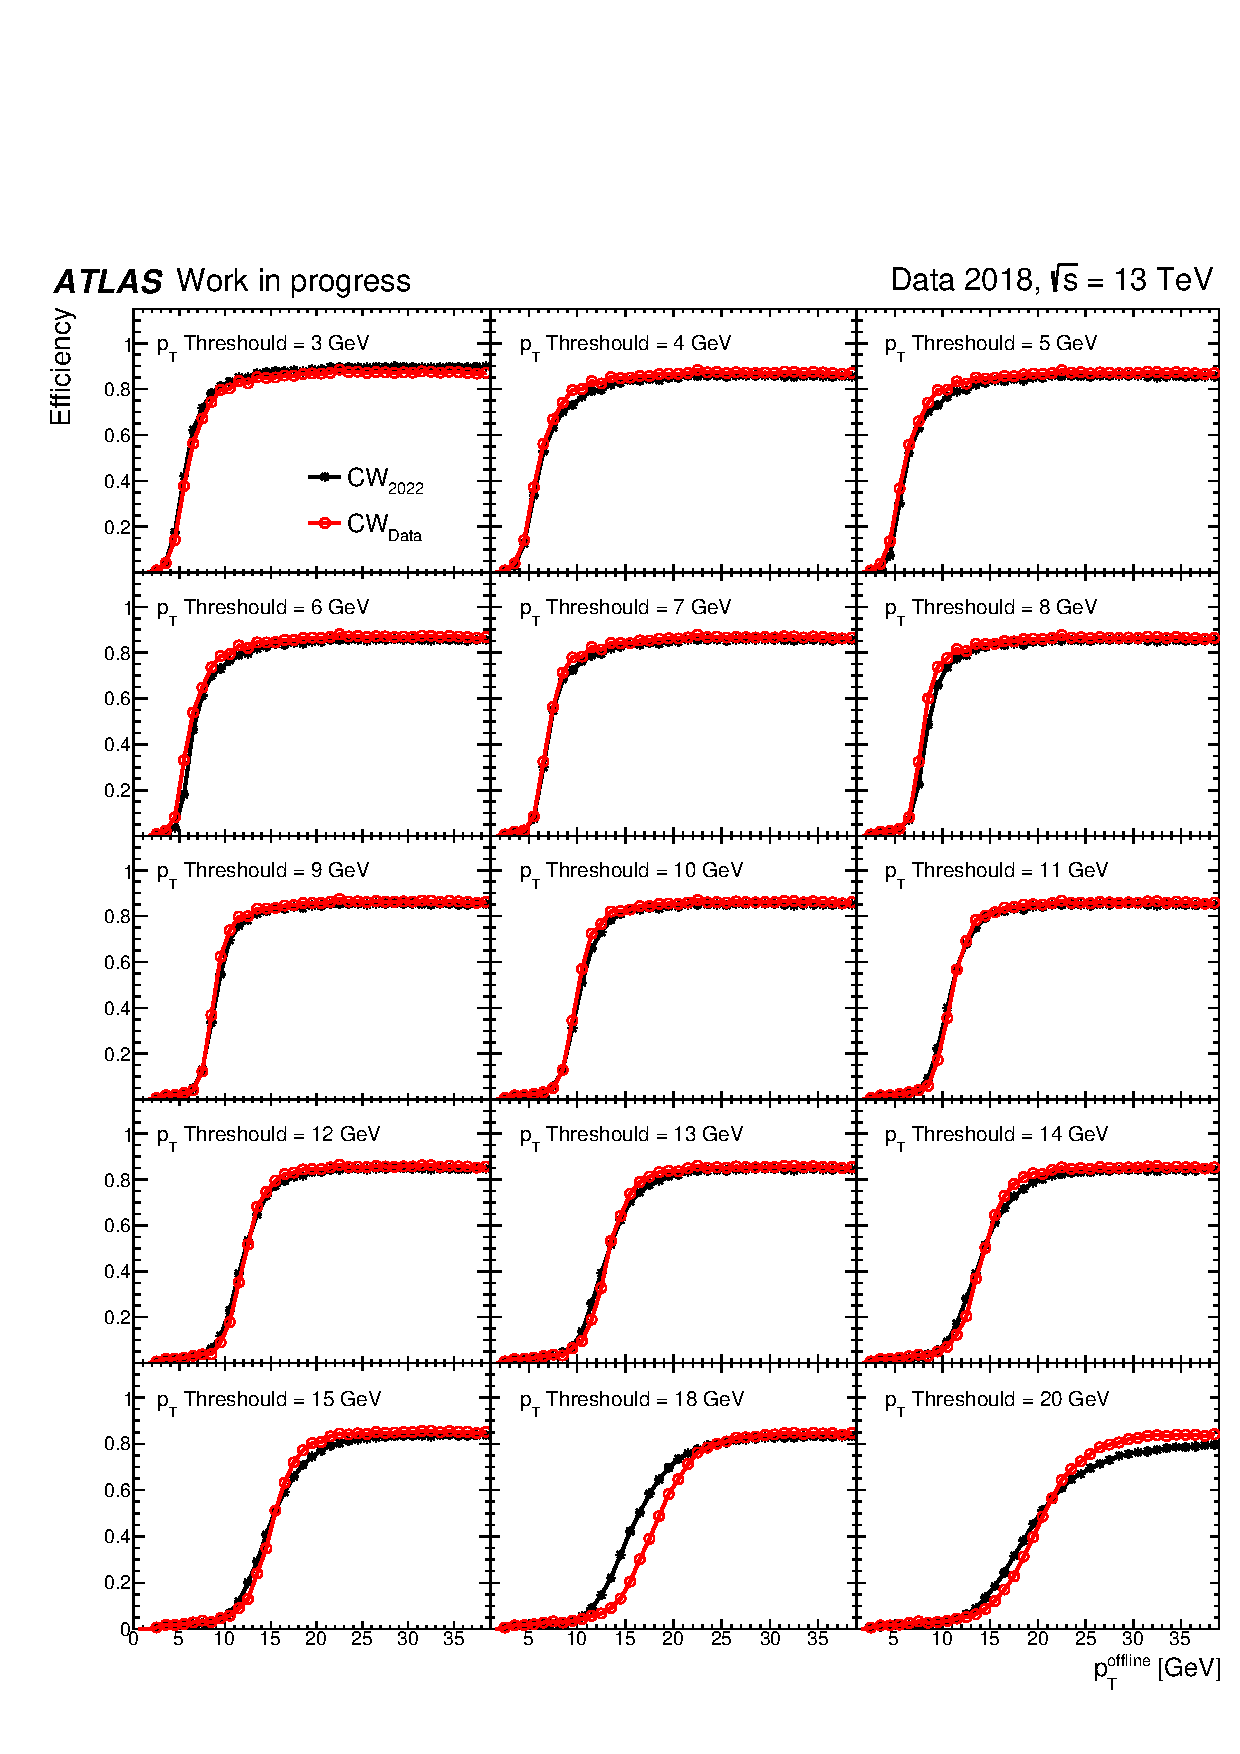
\includegraphics[clip, width=14cm]{fig/5/c1.pdf}
  \caption{$p_{\rm{T}}$閾値3~GeV$\sim$20~GeVにおける$\mathrm{CW_{Data}}$と$\mathrm{CW_{2022}}$のTurn-on curveの比較。評価には2018年Run-2のデータを使用した。}
  \label{fig:v05v06_1_9_Data}
\end{figure}

%\begin{figure}[htb]
%  \centering
%  %\rule{8cm}{6cm}
%  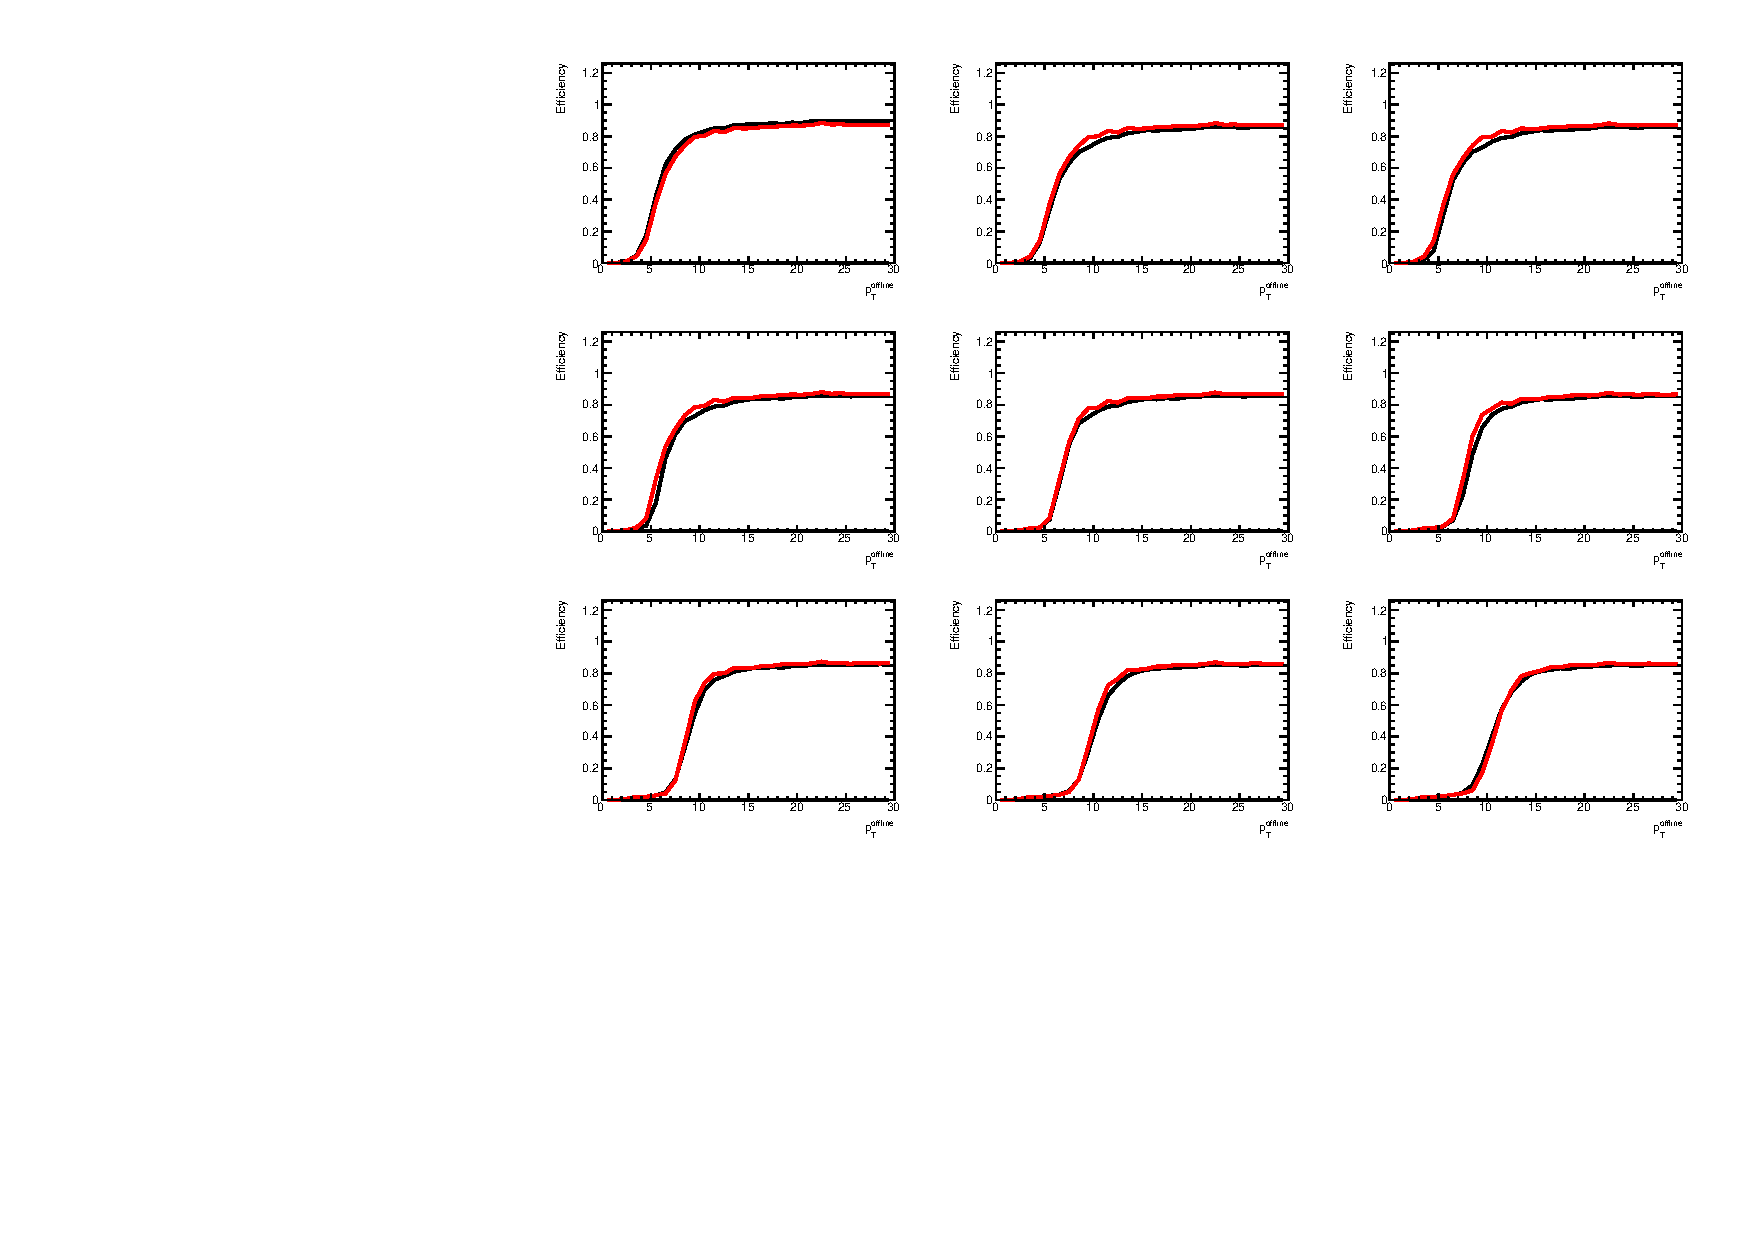
\includegraphics[clip, width=10cm]{fig/5/v05v06_1_9.pdf}
%  \caption{$p_{\rm{T}}$閾値3~GeV$\sim$ 9~GeVにおける$\mathrm{CW_{Data}}$と$\mathrm{CW_{2022}}$のTurn-on curveの比較。評価には2018年Run-3のデータを使用した。}
%  \label{fig:v05v06_1_9_Data}
%\end{figure}

%\begin{figure}[htb]
%  \centering
  %\rule{8cm}{6cm}
%  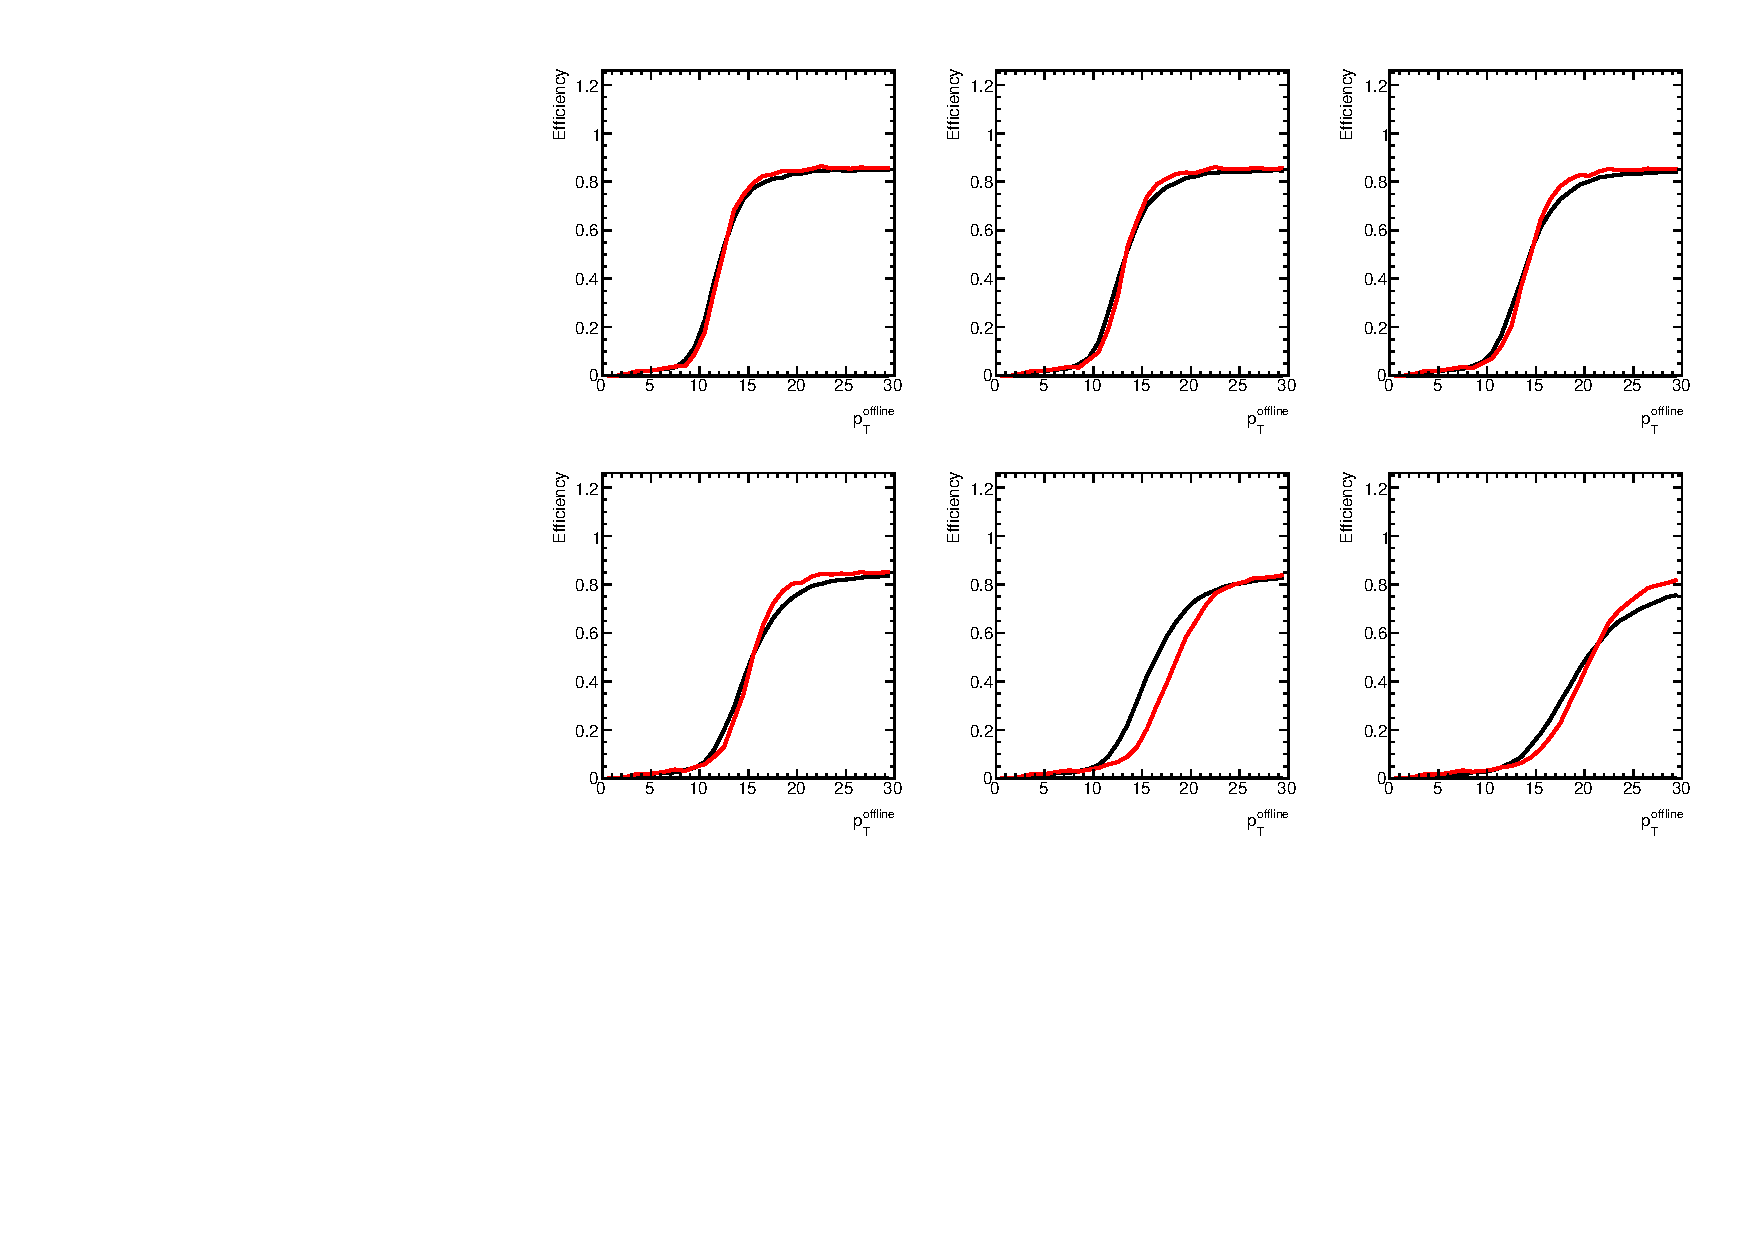
\includegraphics[clip, width=10cm]{fig/5/v05v06_10_15.pdf}
%  \caption{$p_{\rm{T}}$閾値10~GeV$\sim$ 20~GeVにおける$\mathrm{CW_{Data}}$と$\mathrm{CW_{2022}}$のTurn-on curveの比較。評価には2018年Run-3のデータを使用した。}
%  \label{fig:v05v06_10_15_Data}
%\end{figure}

さらに、これらのTurn-on curveに式~\eqref{equ:fitting}によるフィッティングを行い、パラメータの比較を行う。
図~\ref{fig:Resolution_v07v05}に$\mathrm{CW_{Simu}}$と$\mathrm{CW_{2022}}$の各$p_{\rm{T}}$閾値のResolitionの比較、図~\ref{fig:Resolution_v06v05}に$\mathrm{CW_{Data}}$と$\mathrm{CW_{2022}}$の各$p_{\rm{T}}$閾値のResolitionの比較を示す。
また、図~\ref{fig:Plateau_v07v05}に$\mathrm{CW_{Simu}}$と$\mathrm{CW_{2022}}$の各$p_{\rm{T}}$閾値のPlateau Efficiencyの比較、図~\ref{fig:Plateau_v06v05}に$\mathrm{CW_{Data}}$と$\mathrm{CW_{2022}}$の各$p_{\rm{T}}$閾値のPlateau Efficiencyの比較を示す。

まず、シミュレーションデータをトレーニングに用いて作成した$\mathrm{CW_{Simu}}$と2022年Run-3で使用された$\mathrm{CW_{2022}}$を比較すると、Resolition及びPlateau Efficiencyがほとんど一致していることがわかる。
このことから、本研究の手法は従来の手法と同様の性能を維持できるCWの作成が可能であることが確認できた。
次に、実際のデータをトレーニングに使用した$\mathrm{CW_{Data}}$と2022年Run-3で使用された$\mathrm{CW_{2022}}$を比較すると、$p_{\rm{T}}$閾値が14~GeVのトリガーではResolitionが改善され、Plateau Efficiencyが約2$\%$向上したことが見て取れる。これは、実際のデータをトレーニングに用いたことで、検出器アライメントの最適化が行われたことを表している。

\begin{figure}
    %\centering
    \begin{tabular}{cc}
    \centering
    \begin{minipage}[b]{0.45\hsize}%
        \centering
        \hspace*{-1.5cm}
        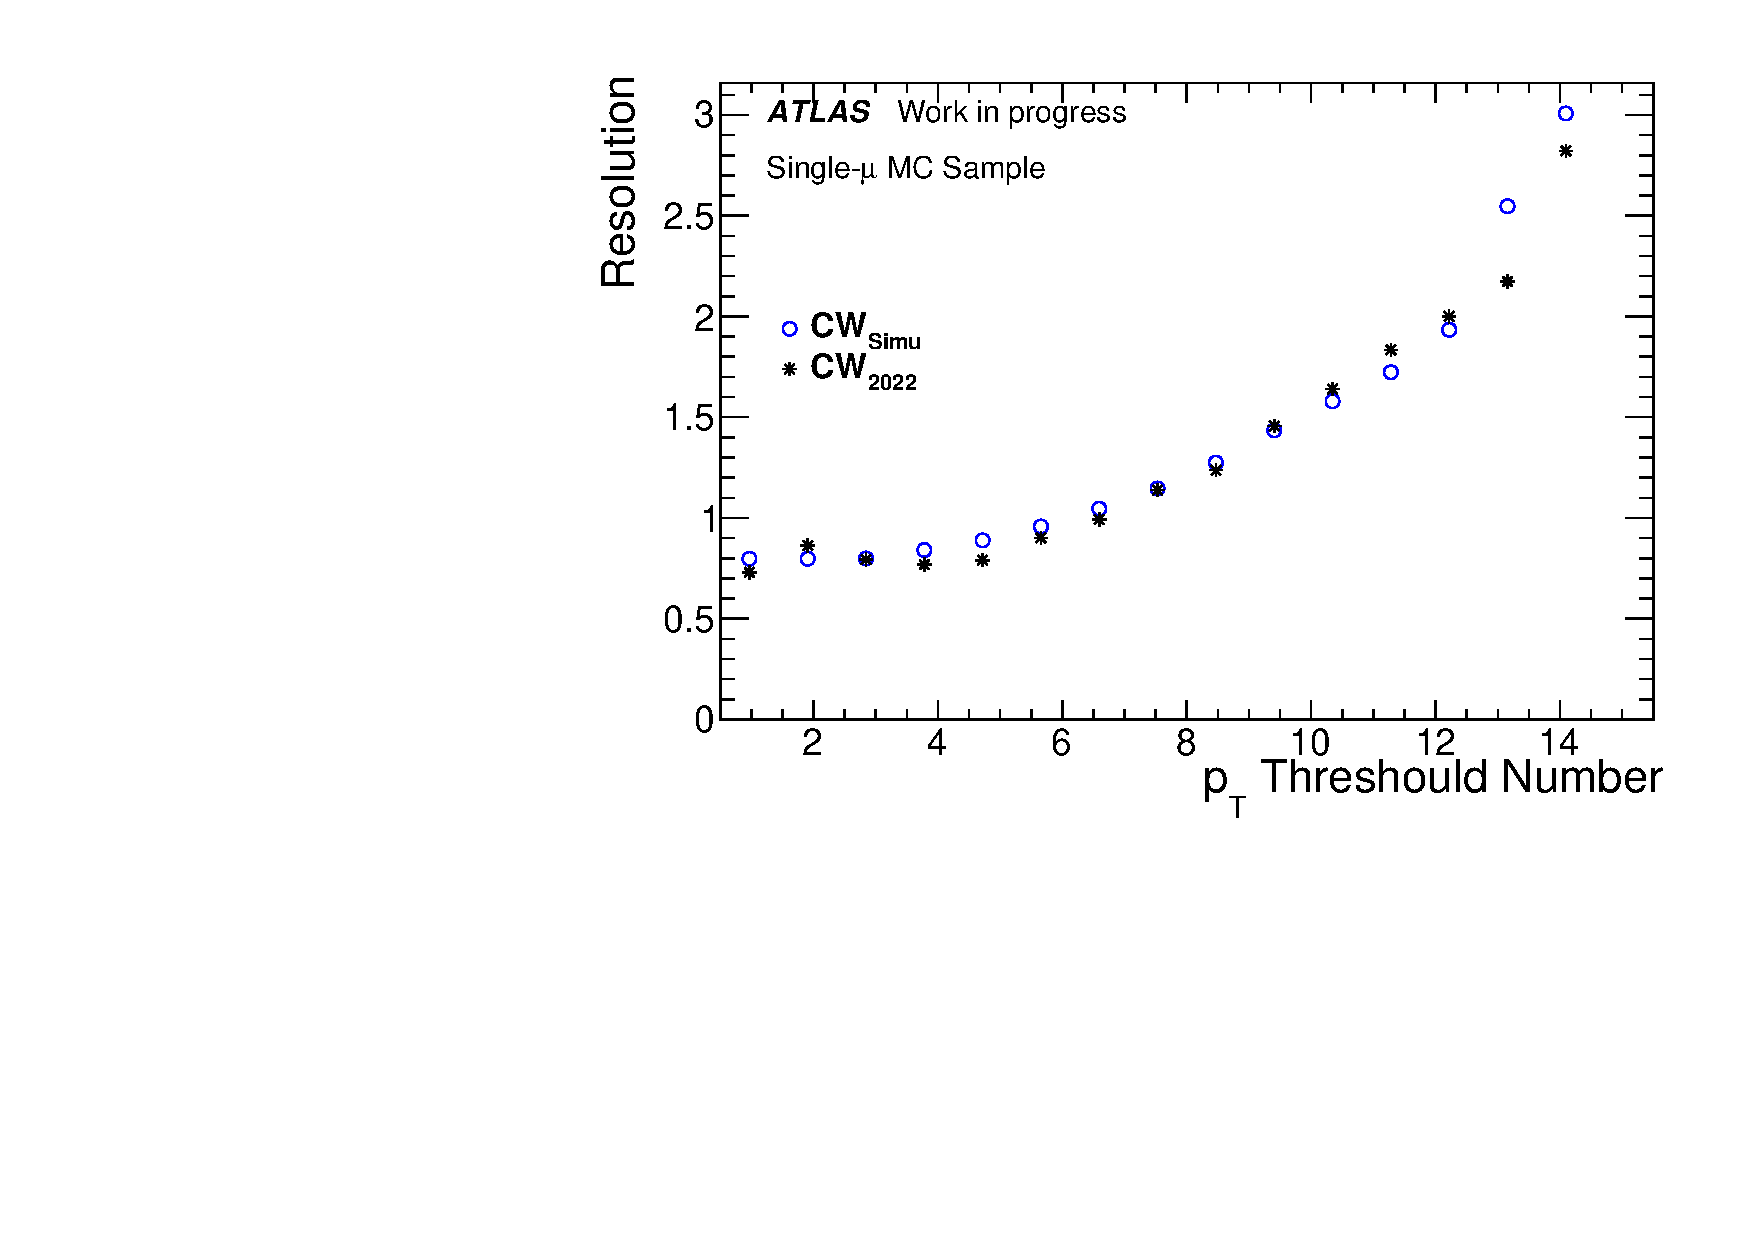
\includegraphics[clip, width=8cm]{fig/5/v05vsv07_Resolution_re.pdf}
        %\vspace{5pt}
        \subcaption{$\mathrm{CW_{Simu}}$と$\mathrm{CW_{2022}}$の比較。}
        \label{fig:Resolution_v07v05}
    \end{minipage}%
    %\hfill
    \begin{minipage}[b]{0.7\hsize}%
        \centering
        \hspace*{-0.75cm}
        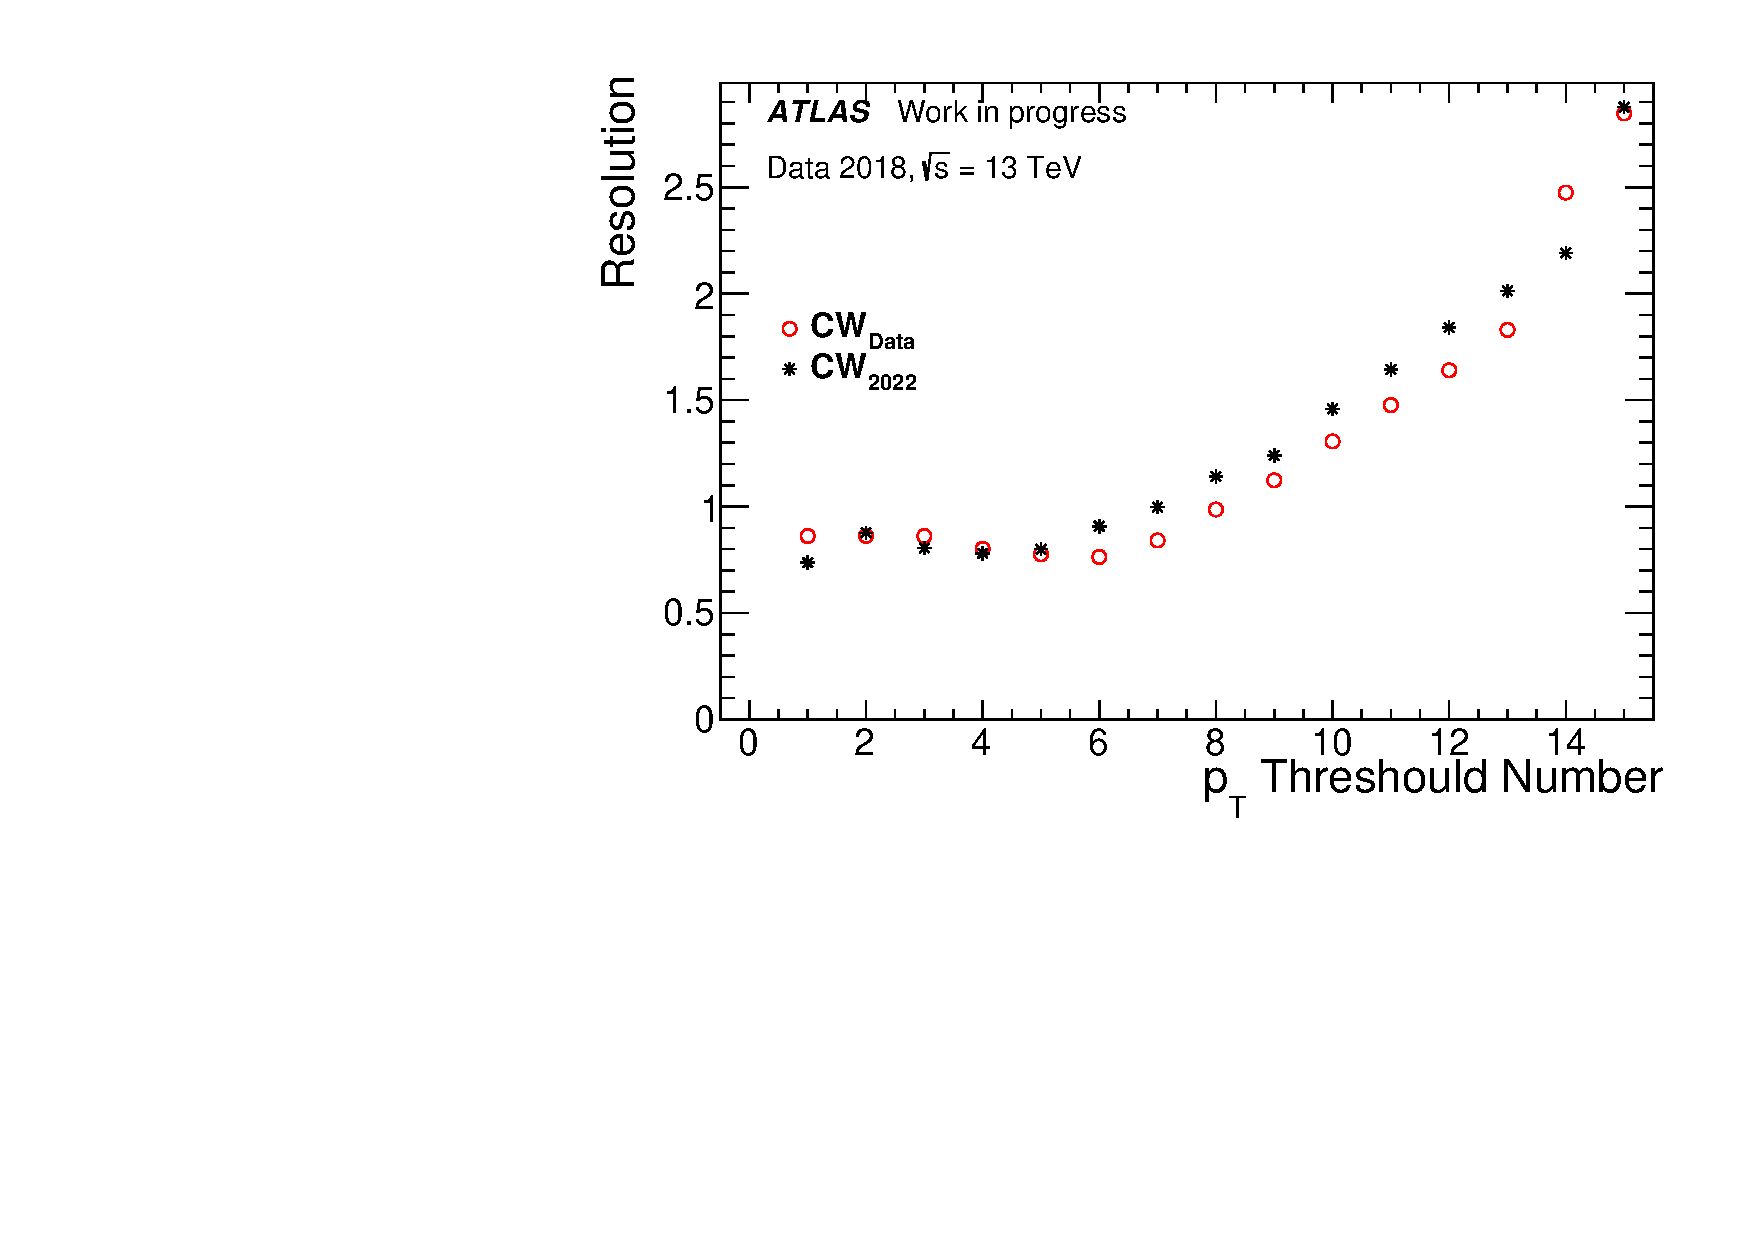
\includegraphics[clip, width=8cm]{fig/5/v05vsv06_Resolution_re.pdf}
        %\vspace{5pt}
        \subcaption{$\mathrm{CW_{Data}}$と$\mathrm{CW_{2022}}$の比較。}
        \label{fig:Resolution_v06v05}
    \end{minipage}%
    \end{tabular}
    \caption{各$p_{\rm{T}}$閾値におけるResolutionの比較。}
    \label{fig:Resolution_v07v06v05}
\end{figure}

\begin{figure}
    %\centering
    \begin{tabular}{cc}
    \centering
    \begin{minipage}[b]{0.45\hsize}%
        \centering
        \hspace*{-1.5cm}
        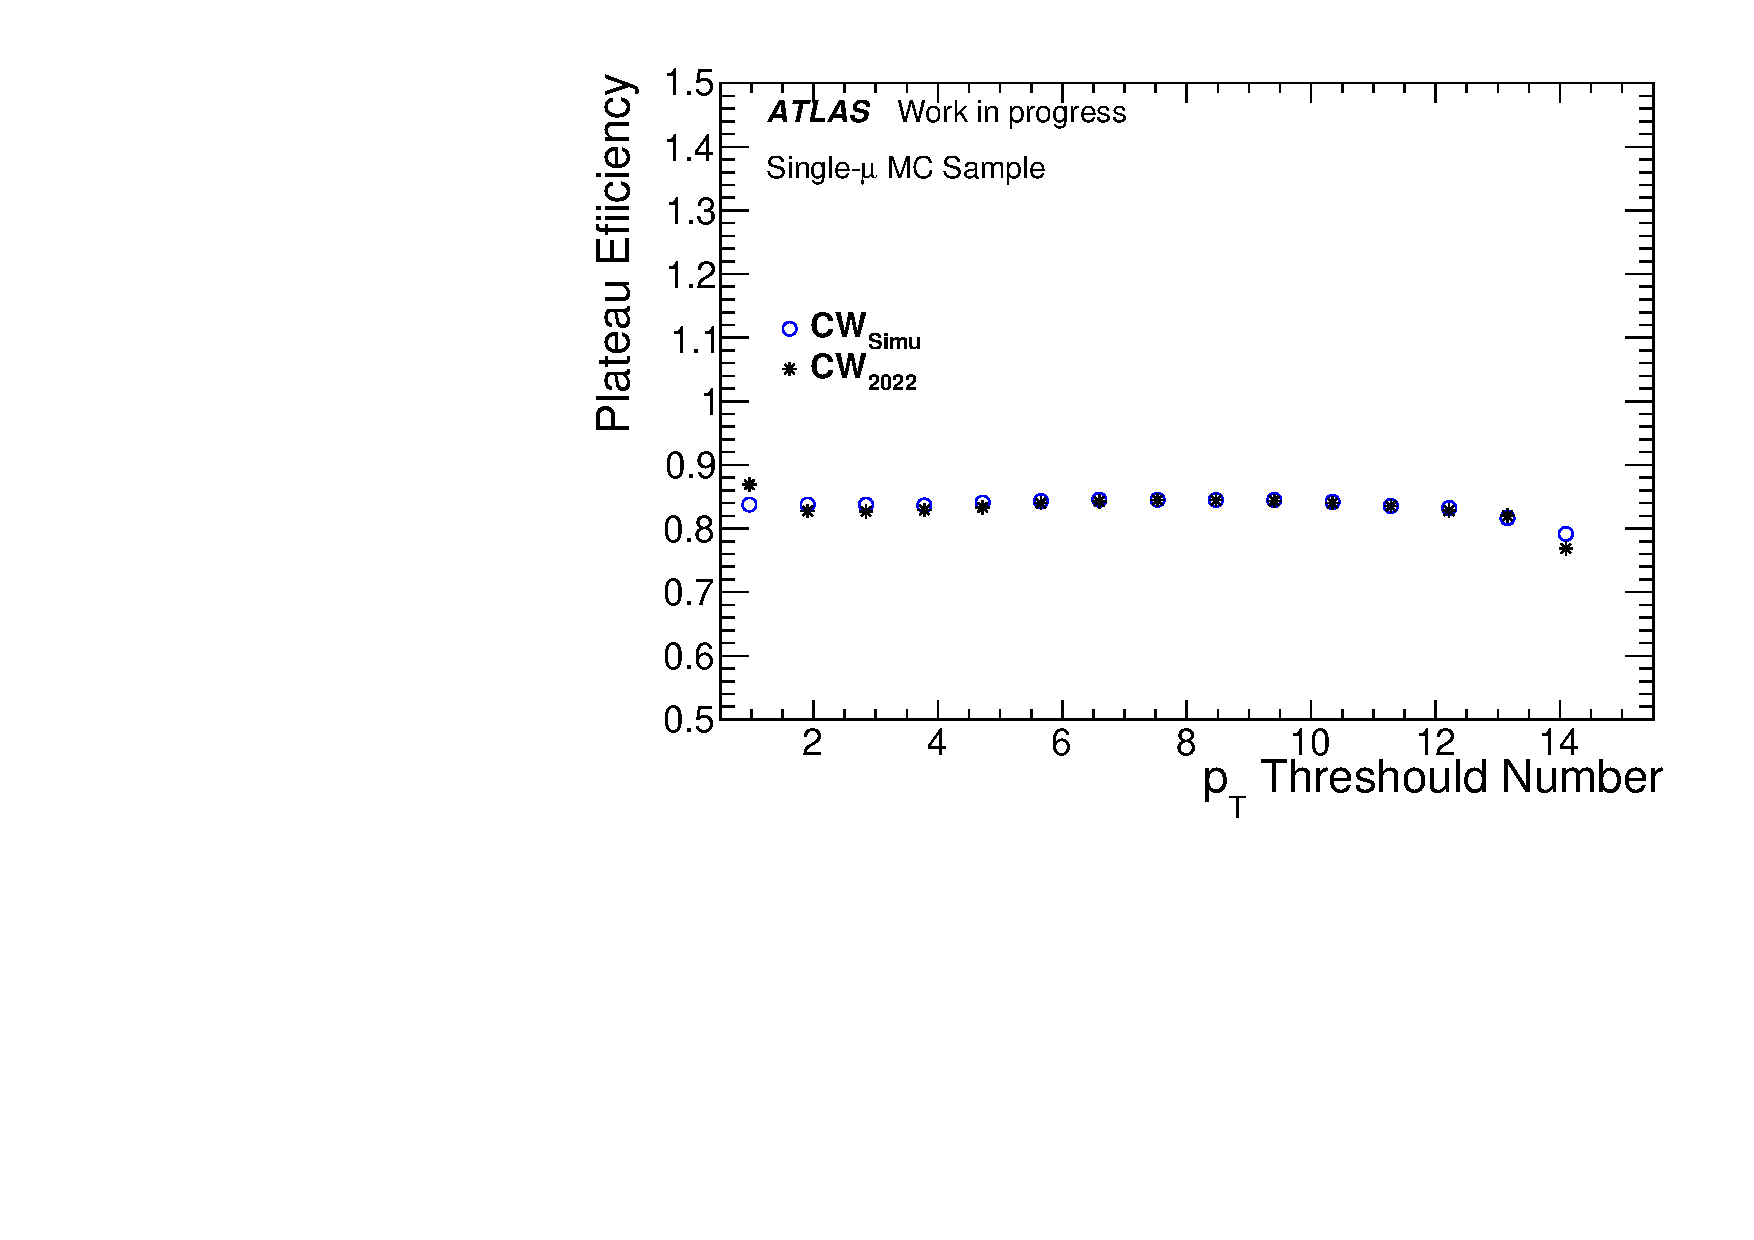
\includegraphics[clip, width=8cm]{fig/5/v05vsv07_Plateau_re.pdf}
        %\vspace{5pt}
        \subcaption{$\mathrm{CW_{Simu}}$と$\mathrm{CW_{2022}}$の比較}
        \label{fig:Plateau_v07v05}
    \end{minipage}%
    %\hfill
    \begin{minipage}[b]{0.7\hsize}%
        \centering
        \hspace*{-0.75cm}
        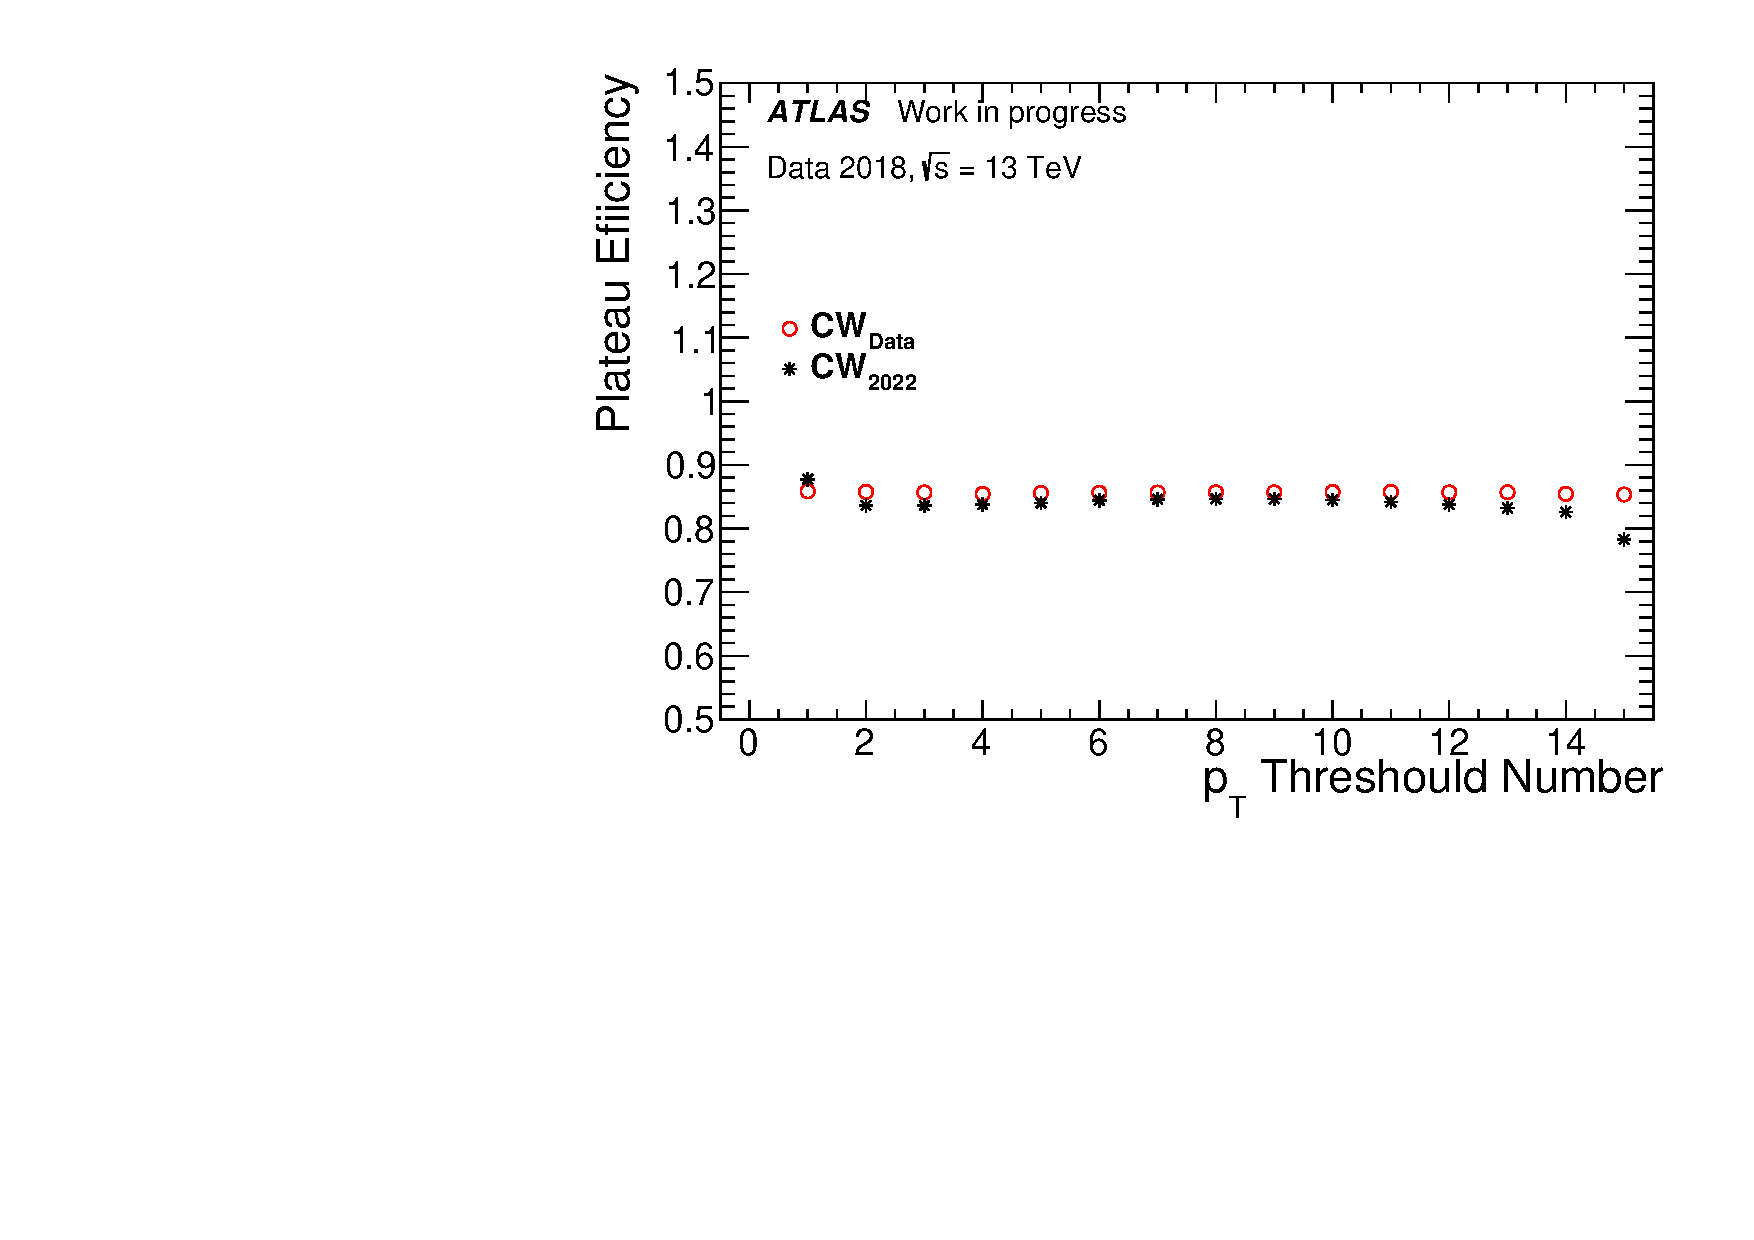
\includegraphics[clip, width=8cm]{fig/5/v05vsv06_Plateau_re.pdf}
        %\vspace{5pt}
        \subcaption{$\mathrm{CW_{Data}}$と$\mathrm{CW_{2022}}$の比較}
        \label{fig:Plateau_v06v05}
    \end{minipage}%
    \end{tabular}
    \caption{各$p_{\rm{T}}$閾値におけるPlateau Efficiencyの比較。}
    \label{fig:Resolution_v07v06v05}
\end{figure}

\subsubsection{$p_{\rm{T}}$判定精度の評価}\label{分解能の評価}
$p_{\rm{T}}$の判定精度を式~\eqref{equ:residual}で計算する$p_{\rm{T}}$ residualを用いて評価する。
\begin{equation}
    (p_{\rm{T}}~{\rm{residual}}) = \frac{p_{\rm{T}}^{\rm{L1}}-p_{\rm{T}}^{\rm{offline}}}{p_{\rm{T}}^{\rm{offline}}}
    \label{equ:residual}
\end{equation}
ここで、$p_{\rm{T}}^{L1}$はL1MuonでCWを用いて判定される$p_{\rm{T}}$閾値、$p_{\rm{T}}^{\rm{offline}}$はオフライン再構成されたミューオンで$p_{\rm{T}}$ある。
そのため、$p_{\rm{T}}^{\rm{offline}}$に対して正しく$p_{\rm{T}}^{L1}$を判定できていれば0に近づき、0から離れるほど$p_{\rm{T}}^{L1}$が$p_{\rm{T}}^{\rm{offline}}$とずれていることを表す。

この$p_{\rm{T}}$ residualを1~GeVごとの$p_{\rm{T}}^{\rm{offline}}$に対して計算し、細かい$p_{\rm{T}}$に対する判定制度の評価を行う。
まず、本研究の手法で作成した$\mathrm{CW_{Simu}}$と2022年度Run-2で使用された$\mathrm{CW_{2022}}$の比較を行う。
図~\ref{residual_MC_3_18}に1~GeVごとの$p_{\rm{T}}^{\rm{offline}}$に対する$p_{\rm{T}}$ residual分布を示す。
\begin{figure}[htbp]
  \centering
  %\rule{8cm}{6cm}
  \hspace*{-1cm}
  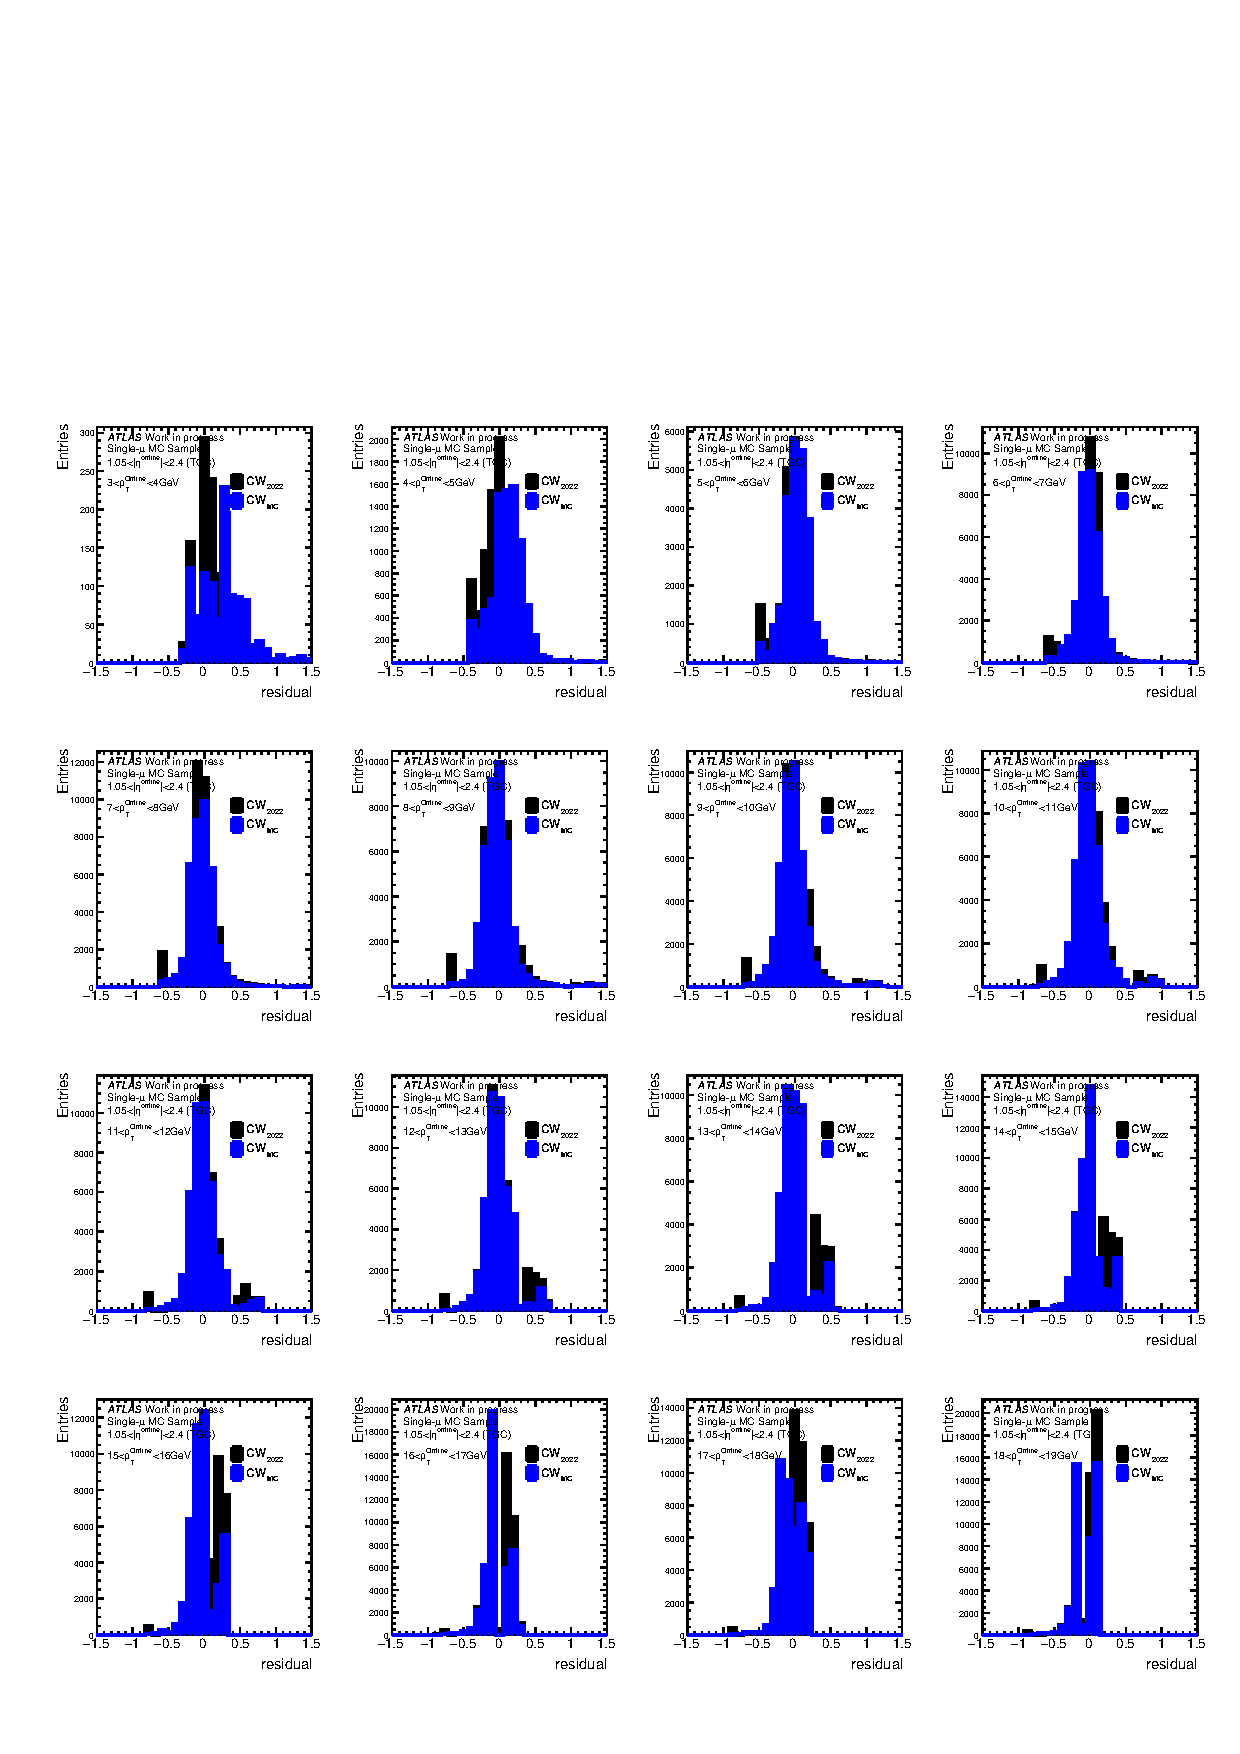
\includegraphics[clip, width=16cm]{fig/5/residual_MC_3_18_re.pdf}
  \caption{TGCにおける1GeV刻みのpT residual分布(3$\sim$18~GeV)。青が本研究の手法で作成した$\mathrm{CW_{Simu}}$を用いた結果、黒が2022年度Run-2で使用された$\mathrm{CW_{2022}}$を用いた結果である。}
  \label{residual_MC_3_18}
\end{figure}
%\begin{figure}[htb]
%  \centering
%  %\rule{8cm}{6cm}
%  \hspace*{-1cm}
%  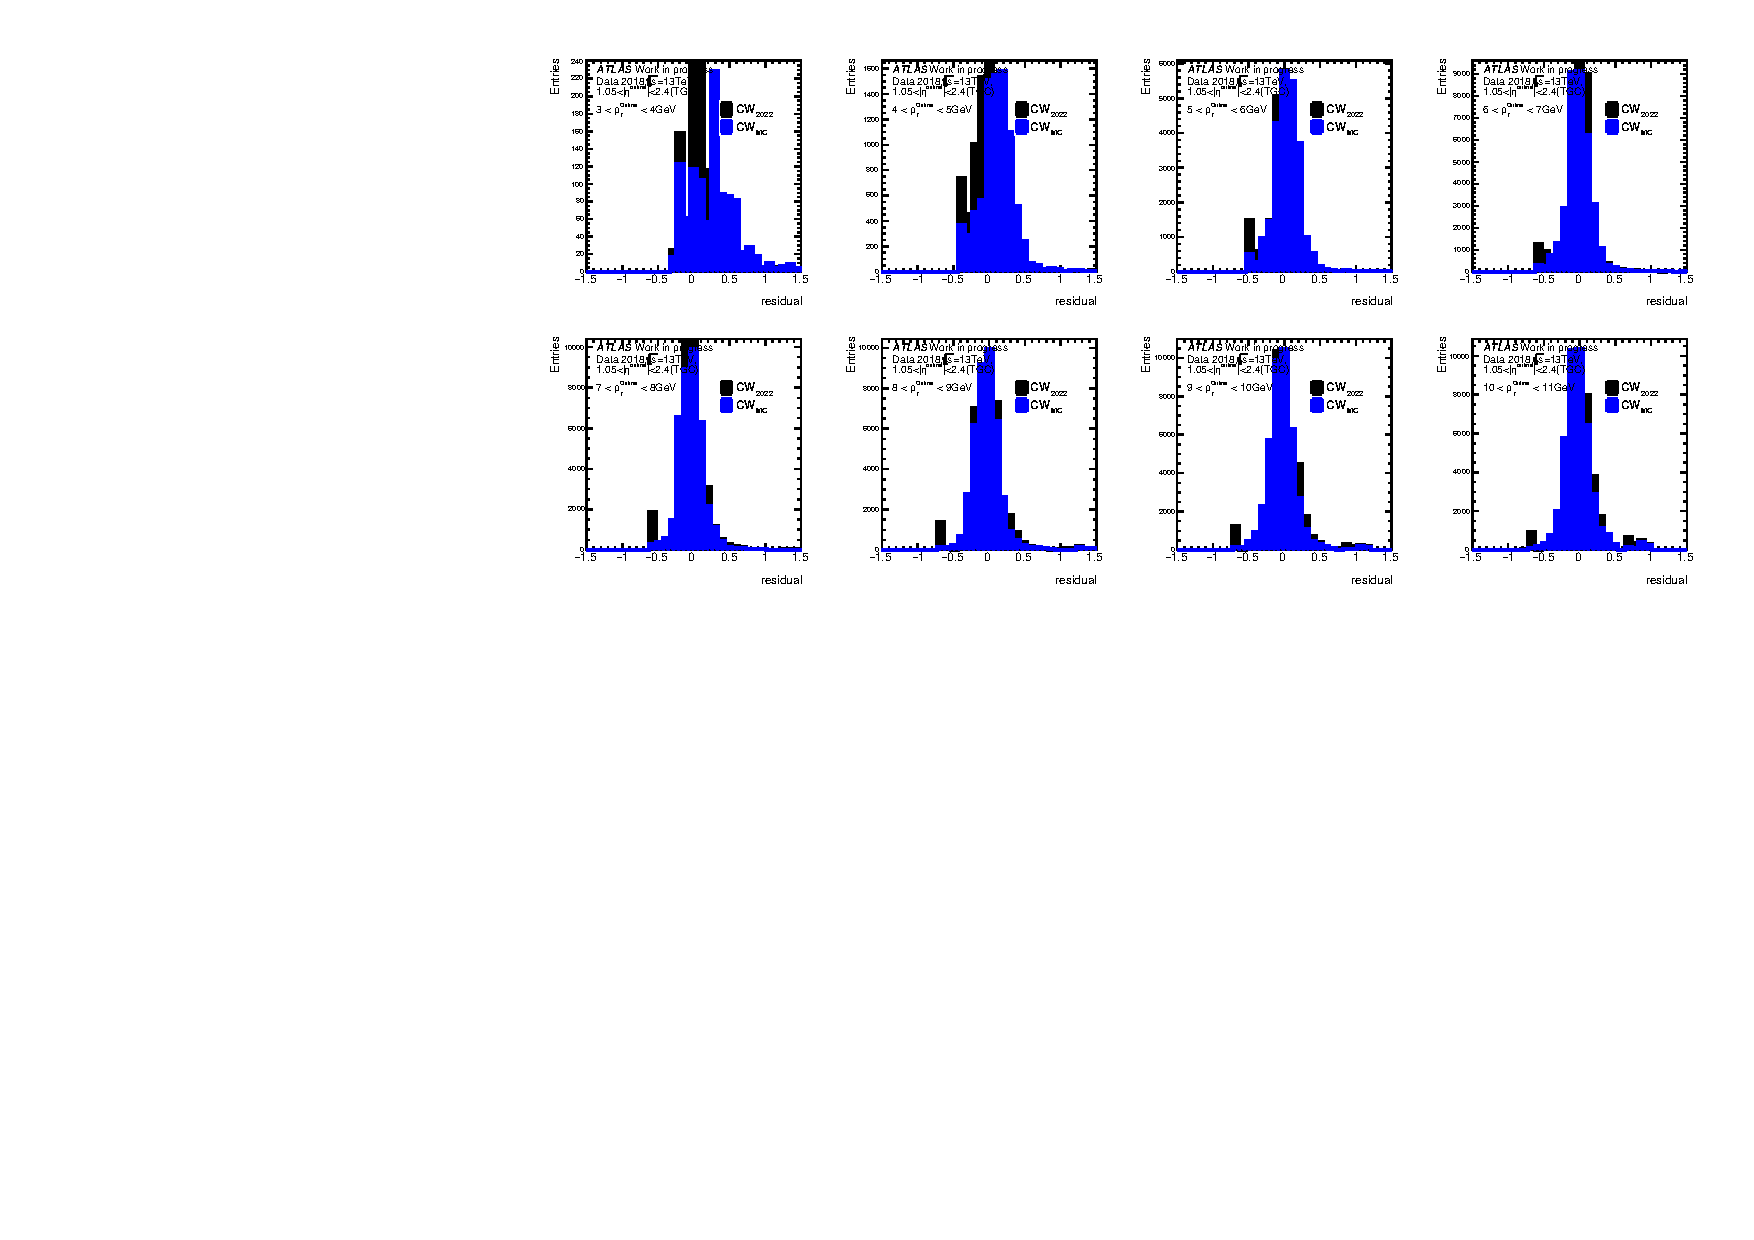
\includegraphics[clip, width=16cm]{fig/5/residual_MC_3_10.pdf}
%  \caption{TGCにおける1GeV刻みのpT residual分布(3$\sim$10~GeV)。青が本研究の手法で作成した$\mathrm{CW_{Simu}}$を用いた結果、黒が2022年度Run-2で使用された$\mathrm{CW_{2022}}$を用いた結果である。}
%  \label{residual_MC_3_10}
%\end{figure}
%\begin{figure}[htb]
%  \centering
  %\rule{8cm}{6cm}
%  \hspace*{-1cm}
%  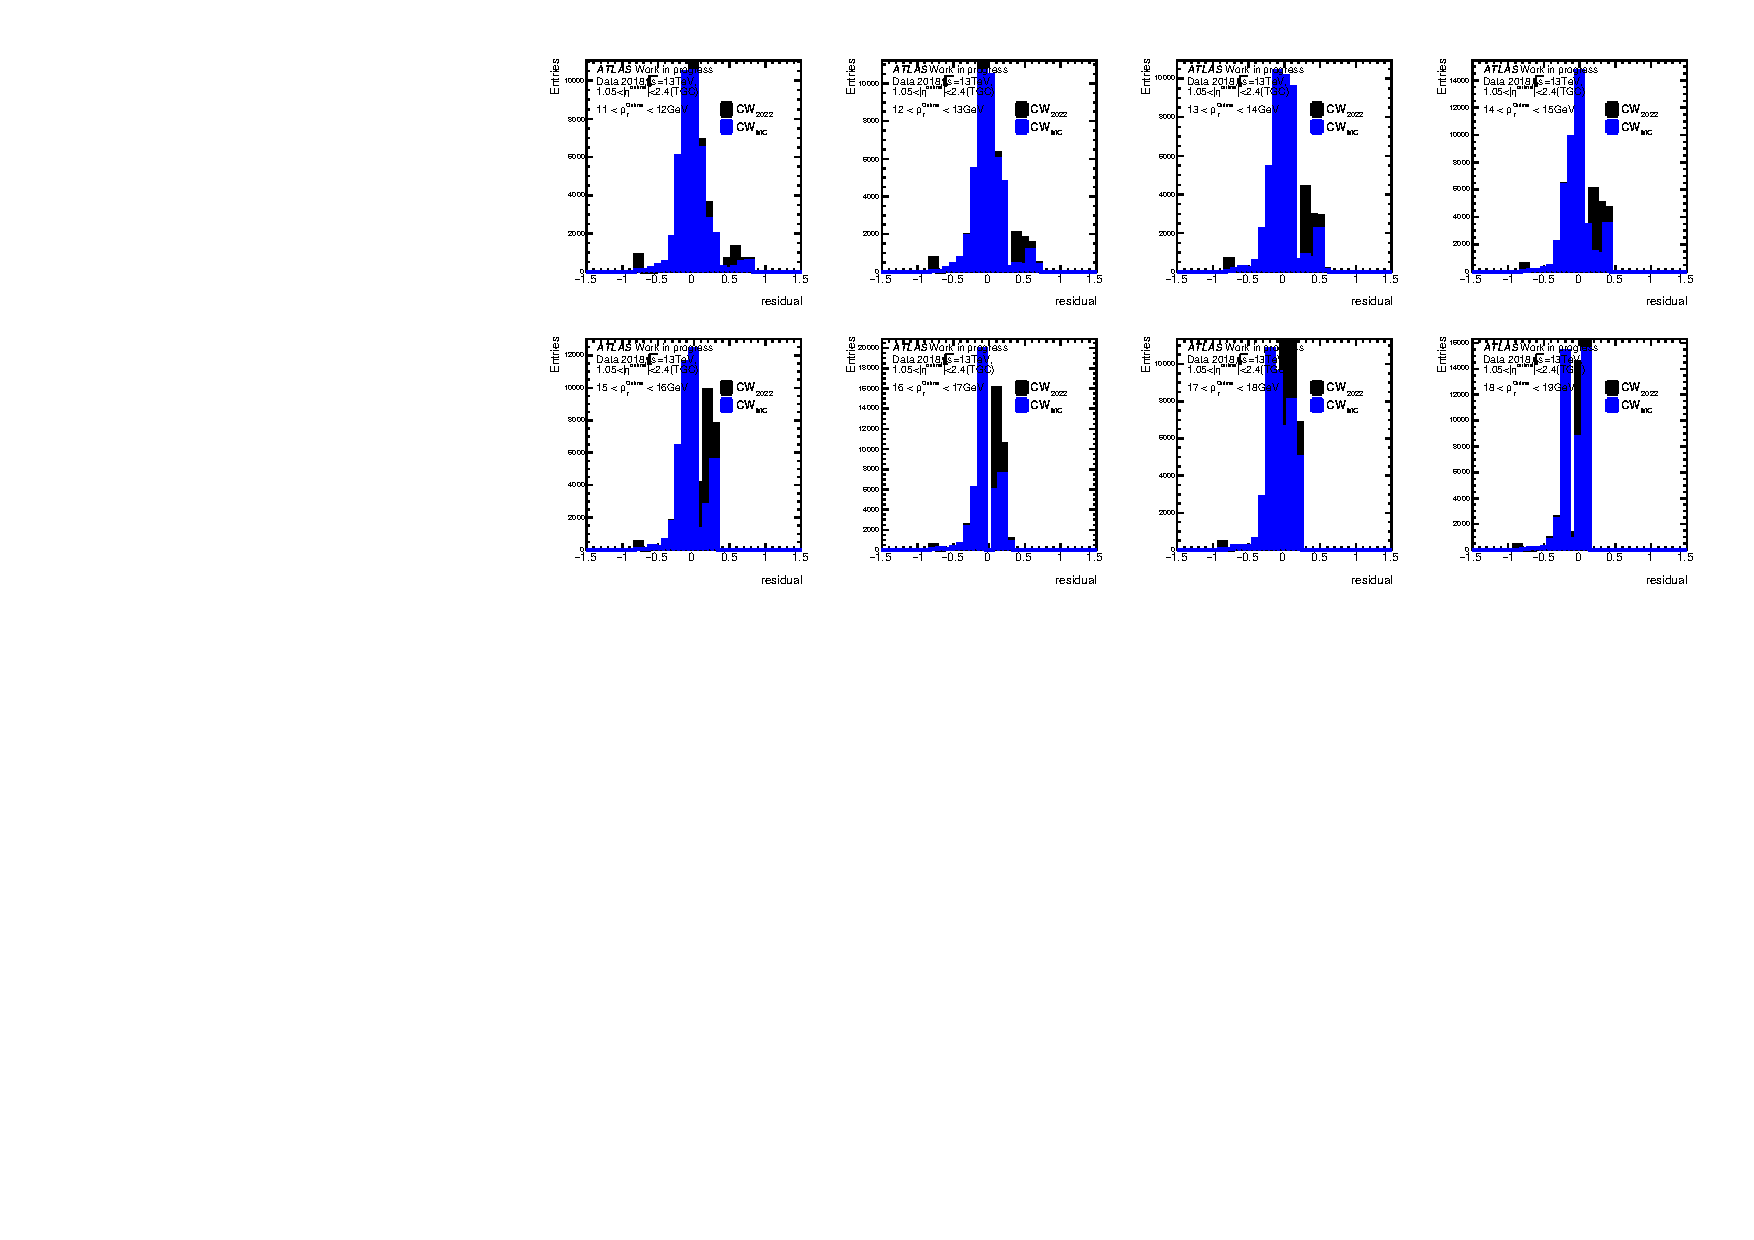
\includegraphics[clip, width=16cm]{fig/5/residual_MC_11_18.pdf}
%  \caption{TGCにおける1GeV刻みのpT residual分布(11$\sim$18~GeV)。青が本研究の手法で作成した$\mathrm{CW_{Simu}}$を用いた結果、黒が2022年度Run-3で使用された$\mathrm{CW_{2022}}$を用いた結果である。}
%  \label{residual_MC_11_18}
%\end{figure}
図~\ref{residual_MC}には1~GeV刻みの$p_{\rm{T}}$ residual分布のMean値と標準偏差を示した。
$\mathrm{CW_{2022}}$と比べ$\mathrm{CW_{Simu}}$は同程度のパフォーマンスが得られることが確認できる。
一方で低い$p_{\rm{T}}$に対する判定精度は$\mathrm{CW_{2022}}$と比べて悪くなっている。これは、$p_{\rm{T}}$閾値の選択方法の影響が表れていると考えられる。
$\mathrm{CW_{2022}}$を作成した先行研究~\cite{article:shiomi-mron}では、この判定精度が向上するような$p_{\rm{T}}$閾値の選択方法を確立し、15段階の$p_{\rm{T}}$閾値を選んでいた。そのため、$\mathrm{CW_{2022}}$と本研究の手法で作成したCWの判定精度と比較すると判定精度が悪くなっている。
しかし本研究の手法は、機械学習の出力からの$p_{\rm{T}}$閾値の選択方法を変えることで、15段階$p_{\rm{T}}$閾値を柔軟に選択できる。そのため、図~\ref{fig:resi_std_Simu}に示すように$\mathrm{CW_{2022}}$と同程度以上の標準偏差を得られていることから、$\mathrm{CW_{2022}}$と同程度の判定精度を持つような$p_{\rm{T}}$閾値を選択できると見込まれる。

\begin{figure}
    %\centering
    \begin{tabular}{cc}
    \begin{minipage}[b]{0.45\hsize}
        %\centering
        \hspace*{-1cm}
        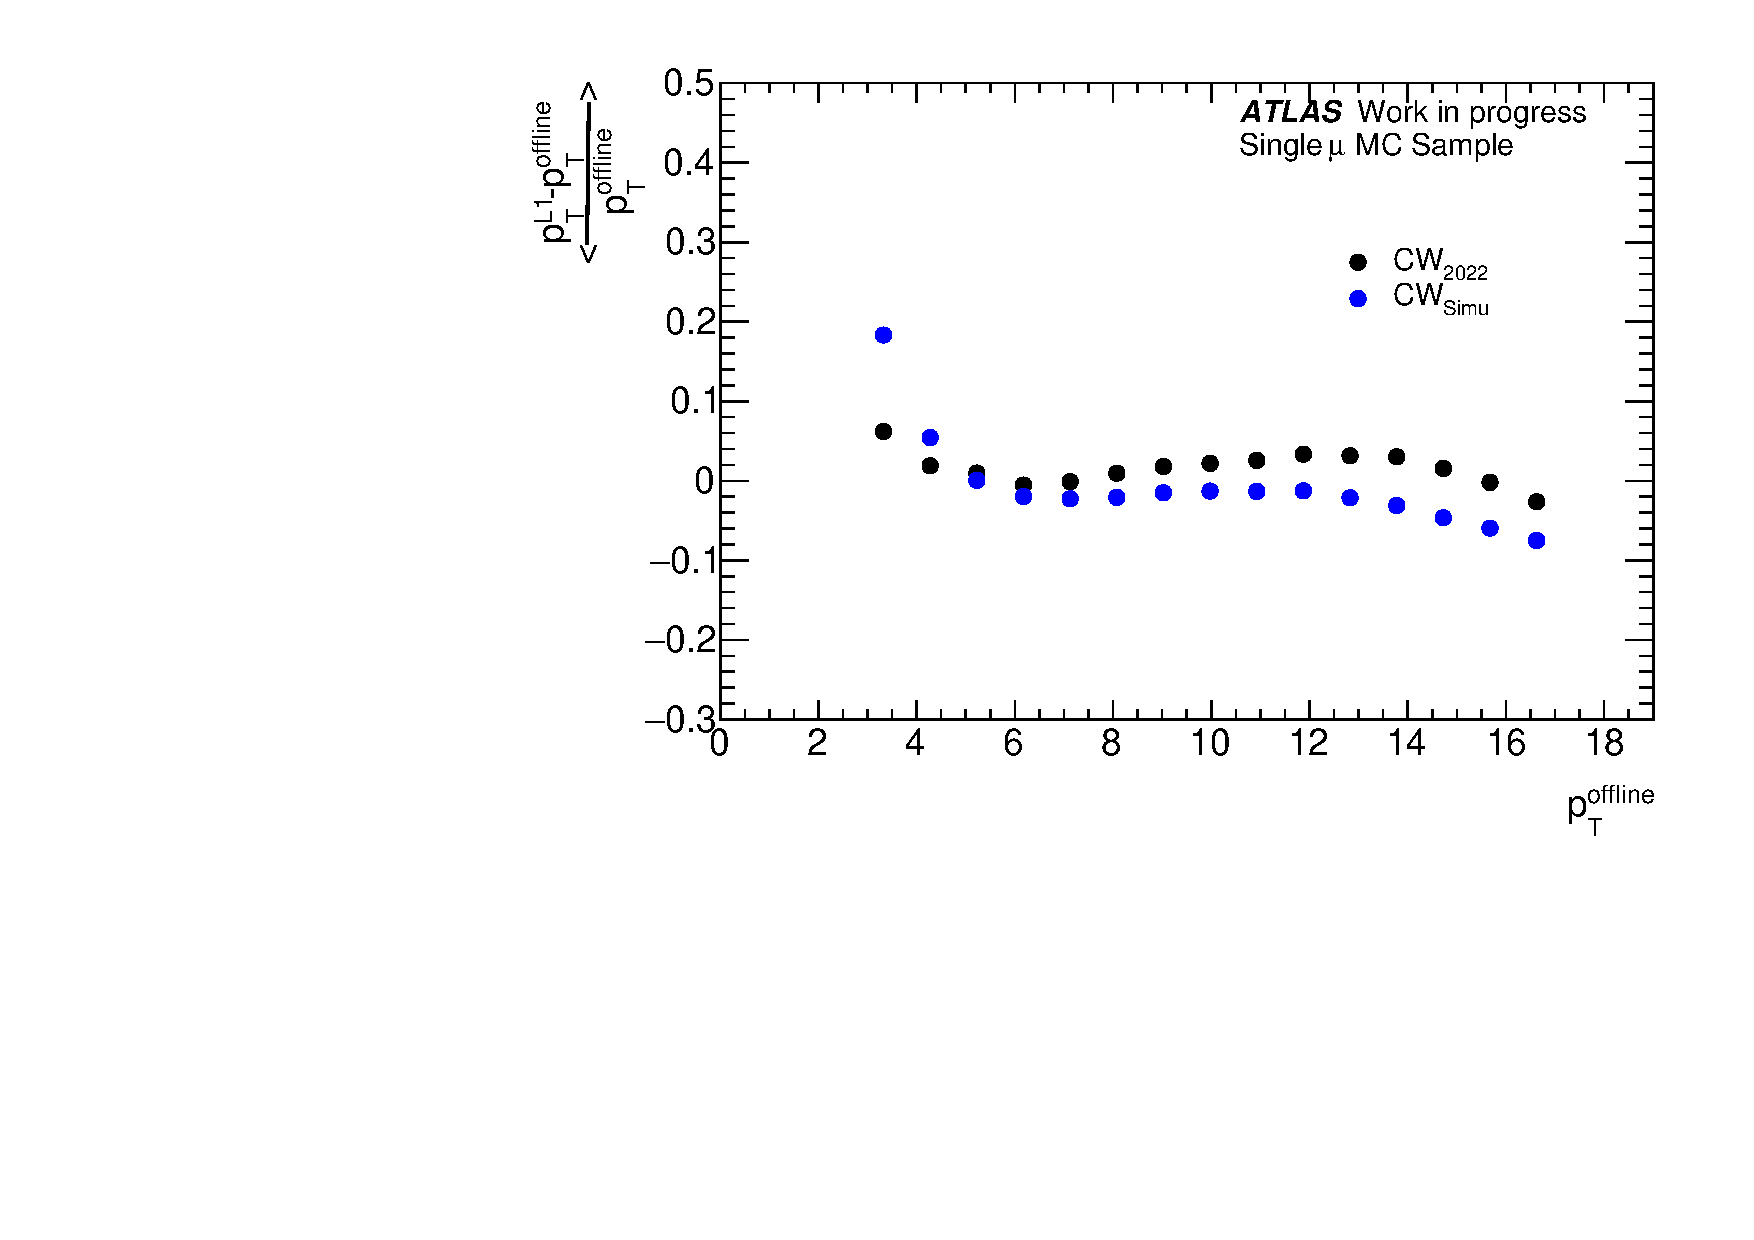
\includegraphics[clip, width=8cm]{fig/5/residual_mean_Simu_re.pdf}
        %\vspace{5pt}
        \subcaption{Mean値}
        \label{fig:resi_mean_Simu}
    \end{minipage}&
    %\hfill
    \begin{minipage}[b]{0.55\hsize}
        %\centering
        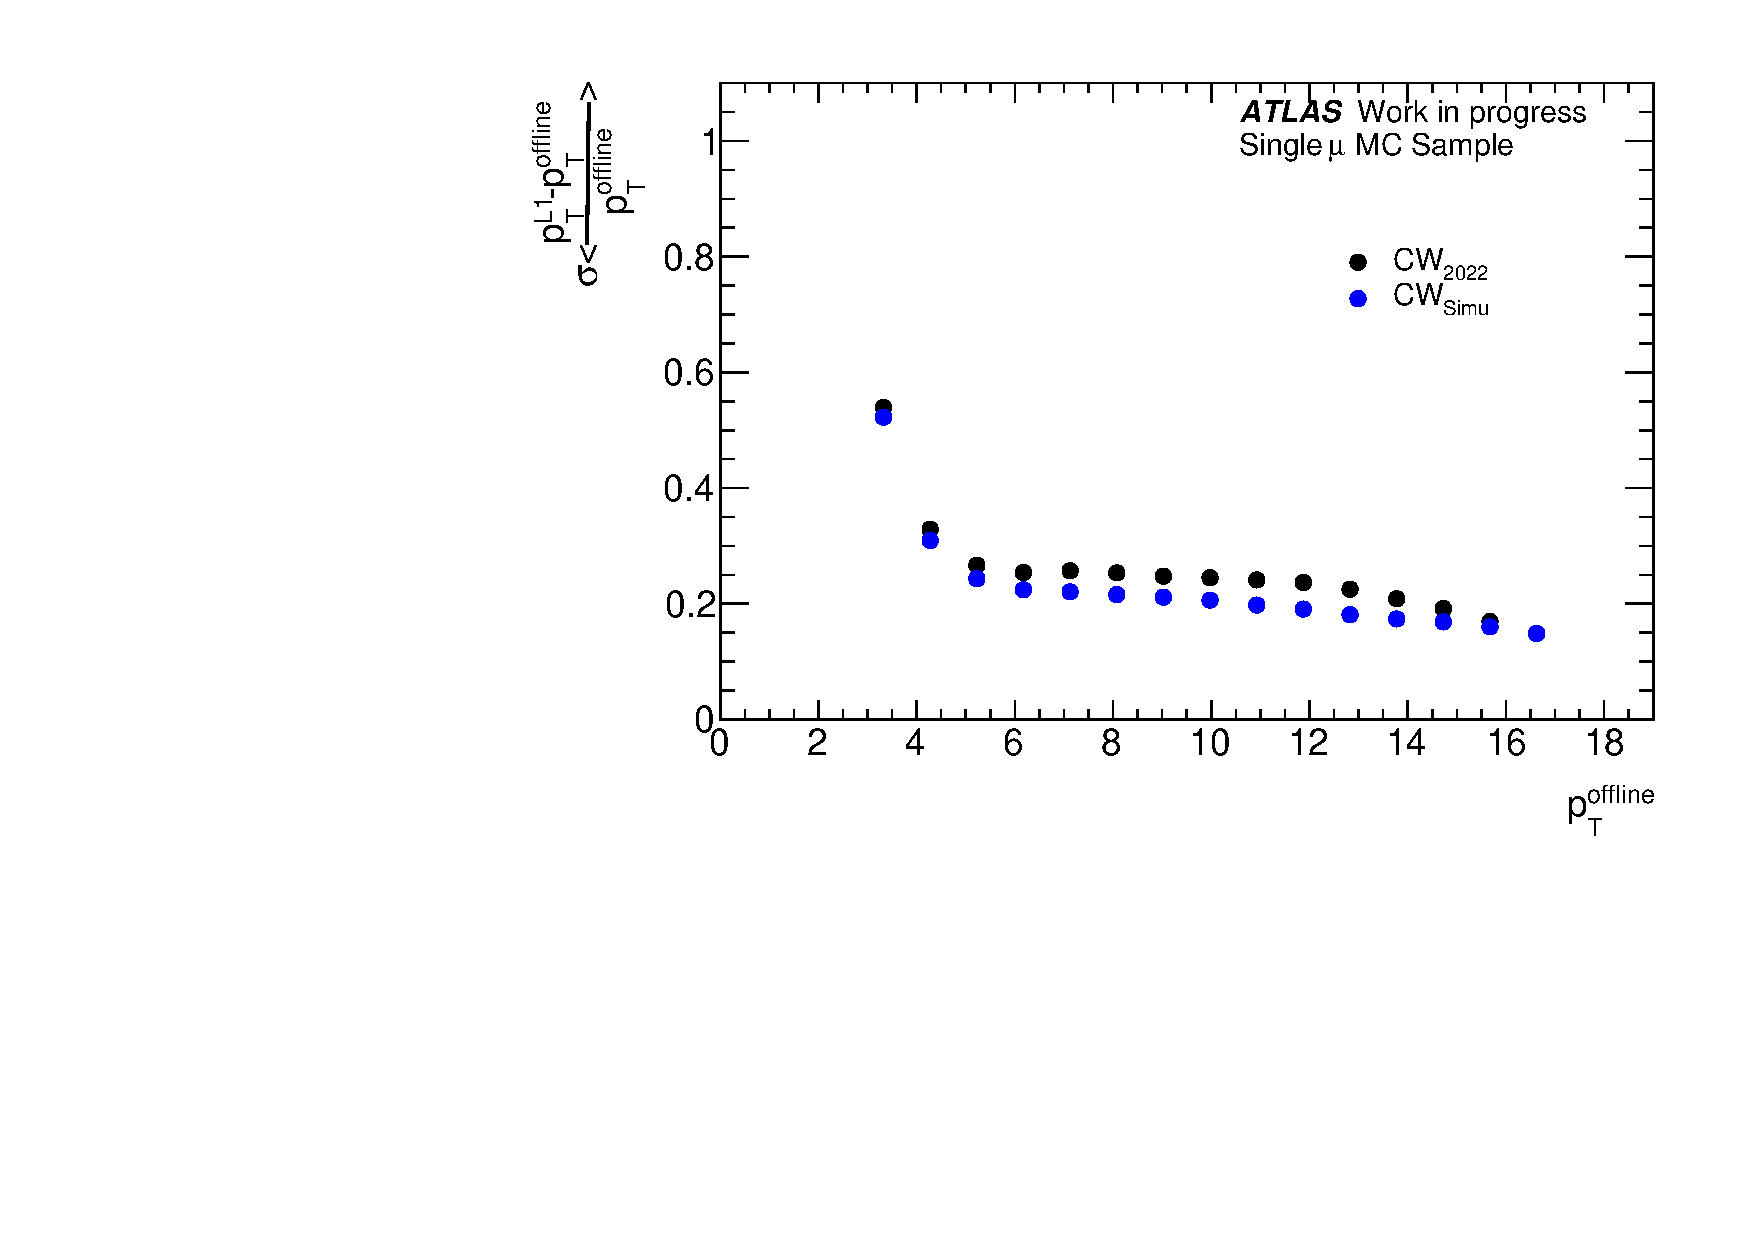
\includegraphics[clip, width=8cm]{fig/5/residual_stdDeVpdf_MC_re.pdf}
        %\vspace{5pt}
        \subcaption{標準偏差}
        \label{fig:resi_std_Simu}
    \end{minipage}
    \end{tabular}
    \caption{本研究の手法で作成した$\mathrm{CW_{Simu}}$と2022年度Run-2で使用された$\mathrm{CW_{2022}}$の$p_{\rm{T}}$ residualの比較。}
    \label{residual_MC}
\end{figure}

同様にして、本研究の手法で作成した$\mathrm{CW_{Data}}$と2022年度Run-2で使用された$\mathrm{CW_{2022}}$の比較を行う。図~\ref{residual_Data_3_18}に1~GeVごとの$p_{\rm{T}}^{\rm{offline}}$に対する$p_{\rm{T}}$ residual分布を示し、図~\ref{residual_Data}には1GeV刻みの$p_{\rm{T}}$ residual分布のMean値と標準偏差を示す。
本研究の手法で作成した$\mathrm{CW_{Data}}$は、2022年度Run-2で使用された$\mathrm{CW_{2022}}$と比べて高い$p_{\rm{T}}$では判定精度の向上が確認できる。一方で、低い$p_{\rm{T}}$における判定精度のmean値が悪くなっているが、標準偏差を比べると改善されていることから、$\mathrm{CW_{Simu}}$の評価で述べたように、機械学習の出力からの$p_{\rm{T}}$閾値の選択方法によって低い$p_{\rm{T}}$における判定精度の改善が見込まれる。
\begin{figure}[htbp]
  \centering
  %\rule{8cm}{6cm}
  \hspace*{-1cm}
  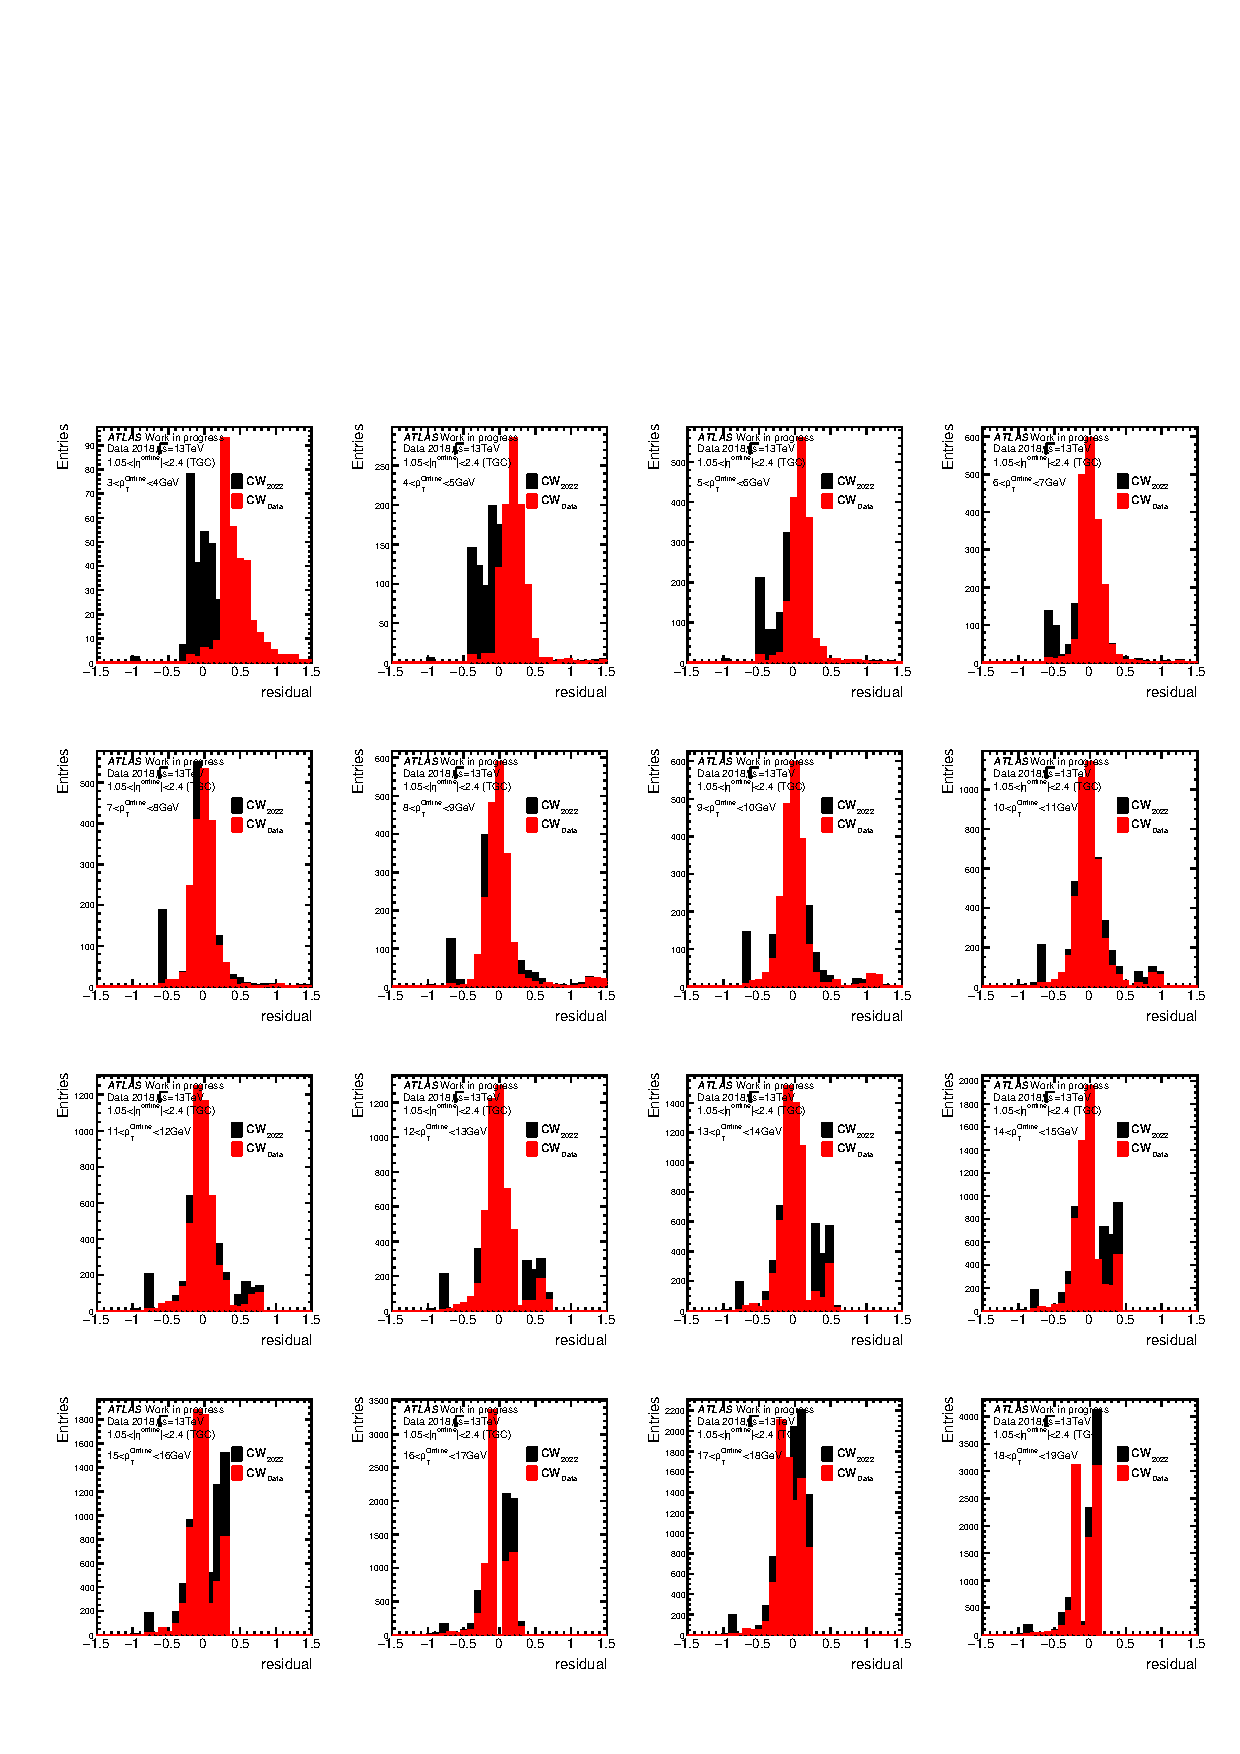
\includegraphics[clip,width=16cm]{fig/5/residual_Data_3_18_re.pdf}
  \caption{TGCにおける1GeV刻みのpT residual分布(3$\sim$18~GeV)。赤が本研究の手法で作成した$\mathrm{CW_{Data}}$を用いた結果、黒が2022年度Run-2で使用された$\mathrm{CW_{2022}}$を用いた結果である。}
  \label{residual_Data_3_18}
\end{figure}

%\begin{figure}[htb]
%  \centering
%  %\rule{8cm}{6cm}
%  \hspace*{-1cm}
%  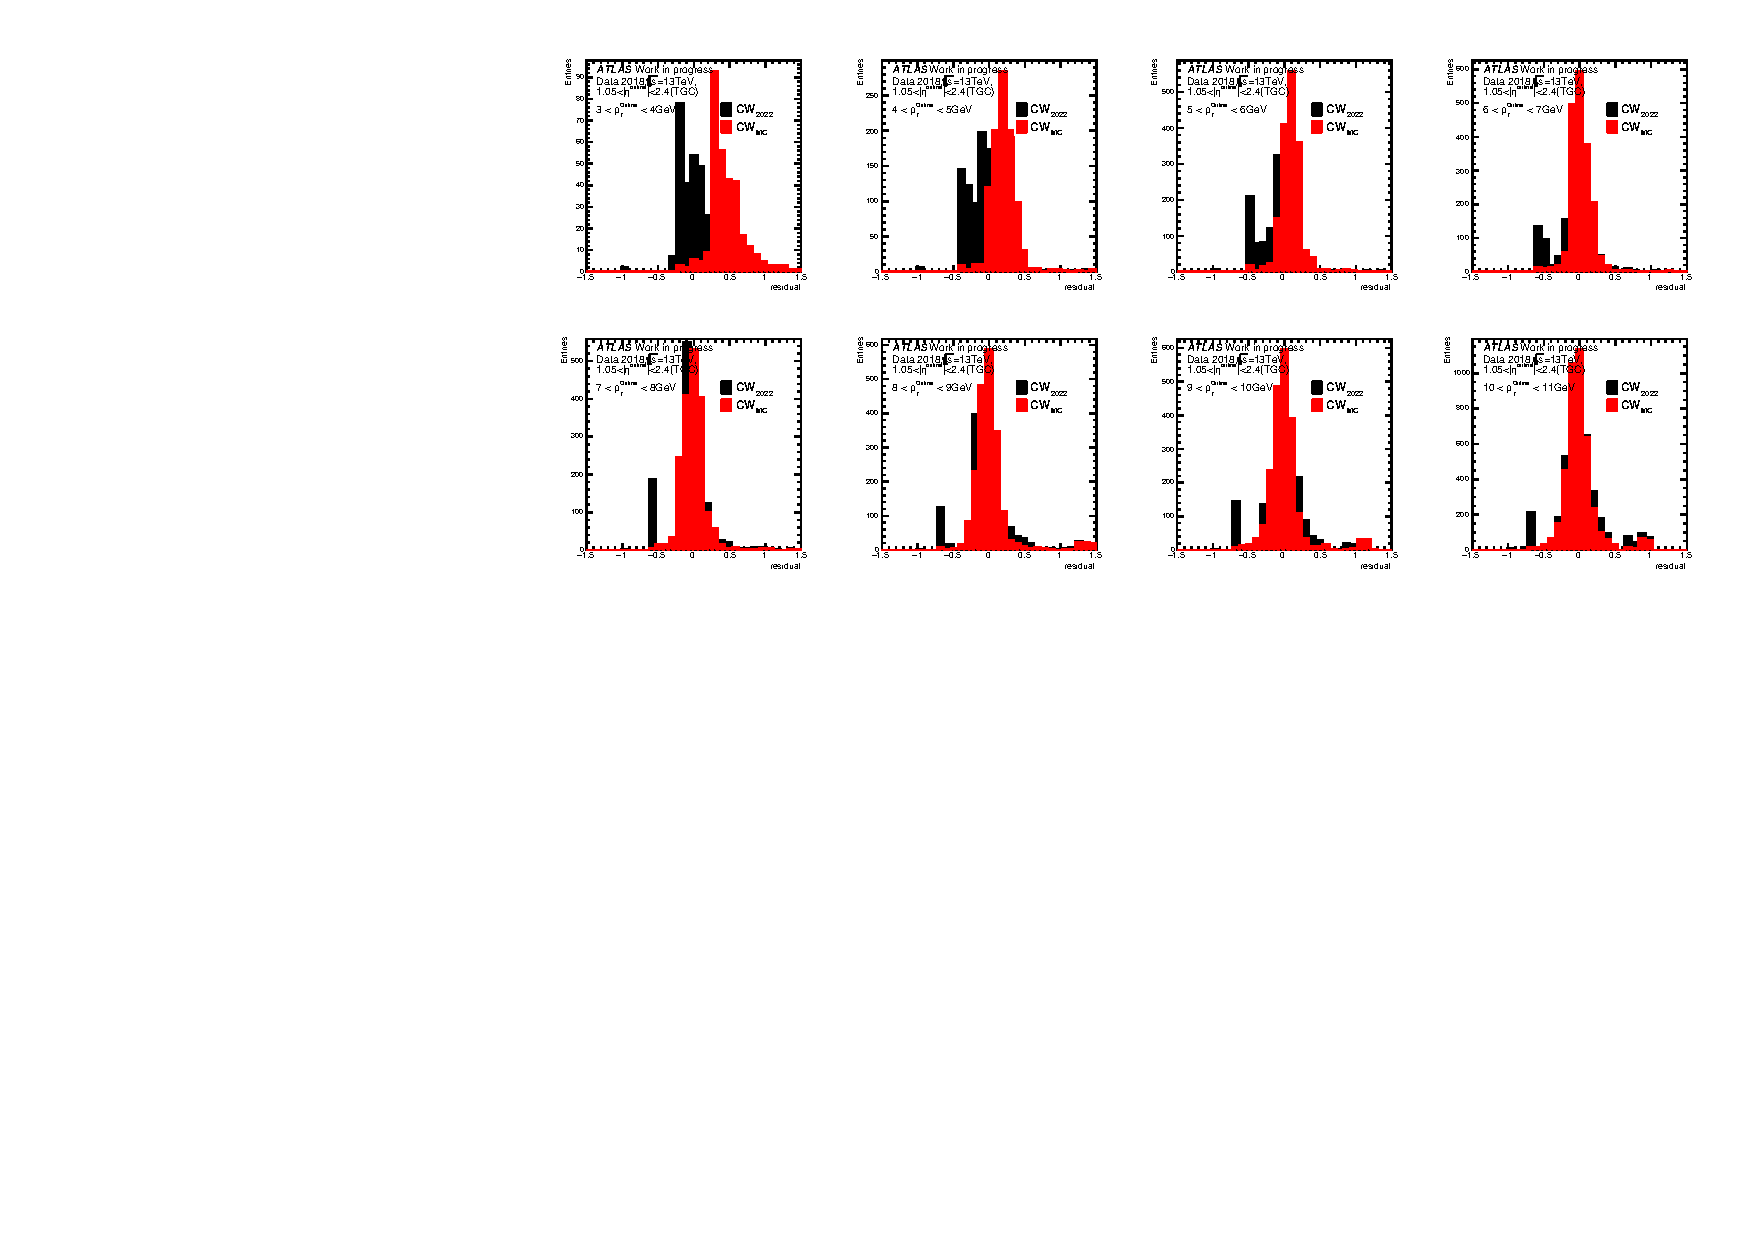
\includegraphics[clip, width=16cm]{fig/5/residual_Data_3_10.pdf}
%  \caption{TGCにおける1GeV刻みのpT residual分布(3$\sim$10~GeV)。赤が本研究の手法で作成した$\mathrm{CW_{Data}}$を用いた結果、黒が2022年度Run-2で使用された$\mathrm{CW_{2022}}$を用いた結果である。}
%  \label{residual_Data_3_10}
%\end{figure}
%\begin{figure}[htb]
%  \centering
%  %\rule{8cm}{6cm}
%  \hspace*{-1cm}
%  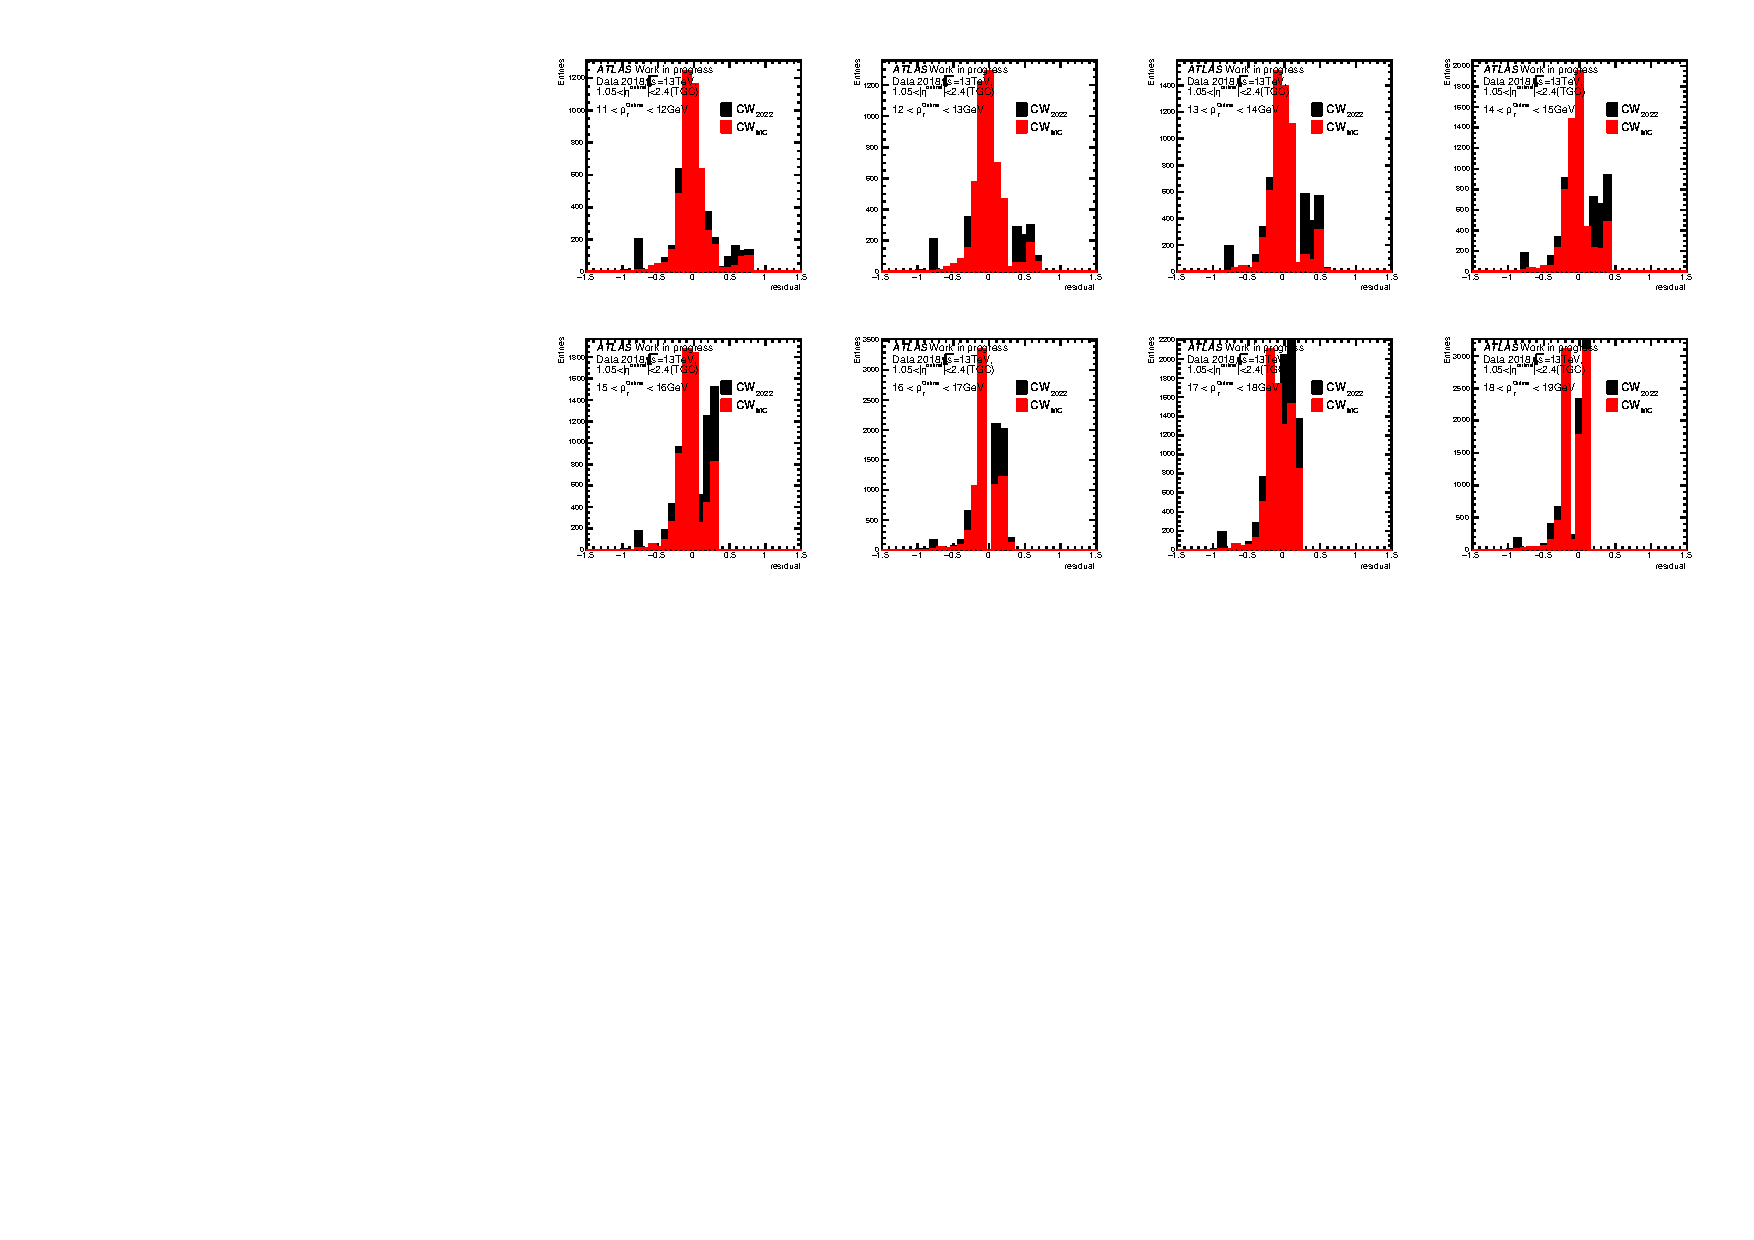
\includegraphics[clip, width=16cm]{fig/5/residual_Data_11_18.pdf}
%  \caption{TGCにおける1GeV刻みのpT residual分布(11$\sim$18~GeV)。赤が本研究の手法で作成した$\mathrm{CW_{Data}}$を用いた結果、黒が2022年度Run-2で使用された$\mathrm{CW_{2022}}$を用いた結果である。}
%  \label{residual_Data_11_18}
%\end{figure}



\begin{figure}
    %\centering
    \begin{tabular}{cc}
    \begin{minipage}[b]{0.45\hsize}
        %\centering
        \hspace*{-1cm}
        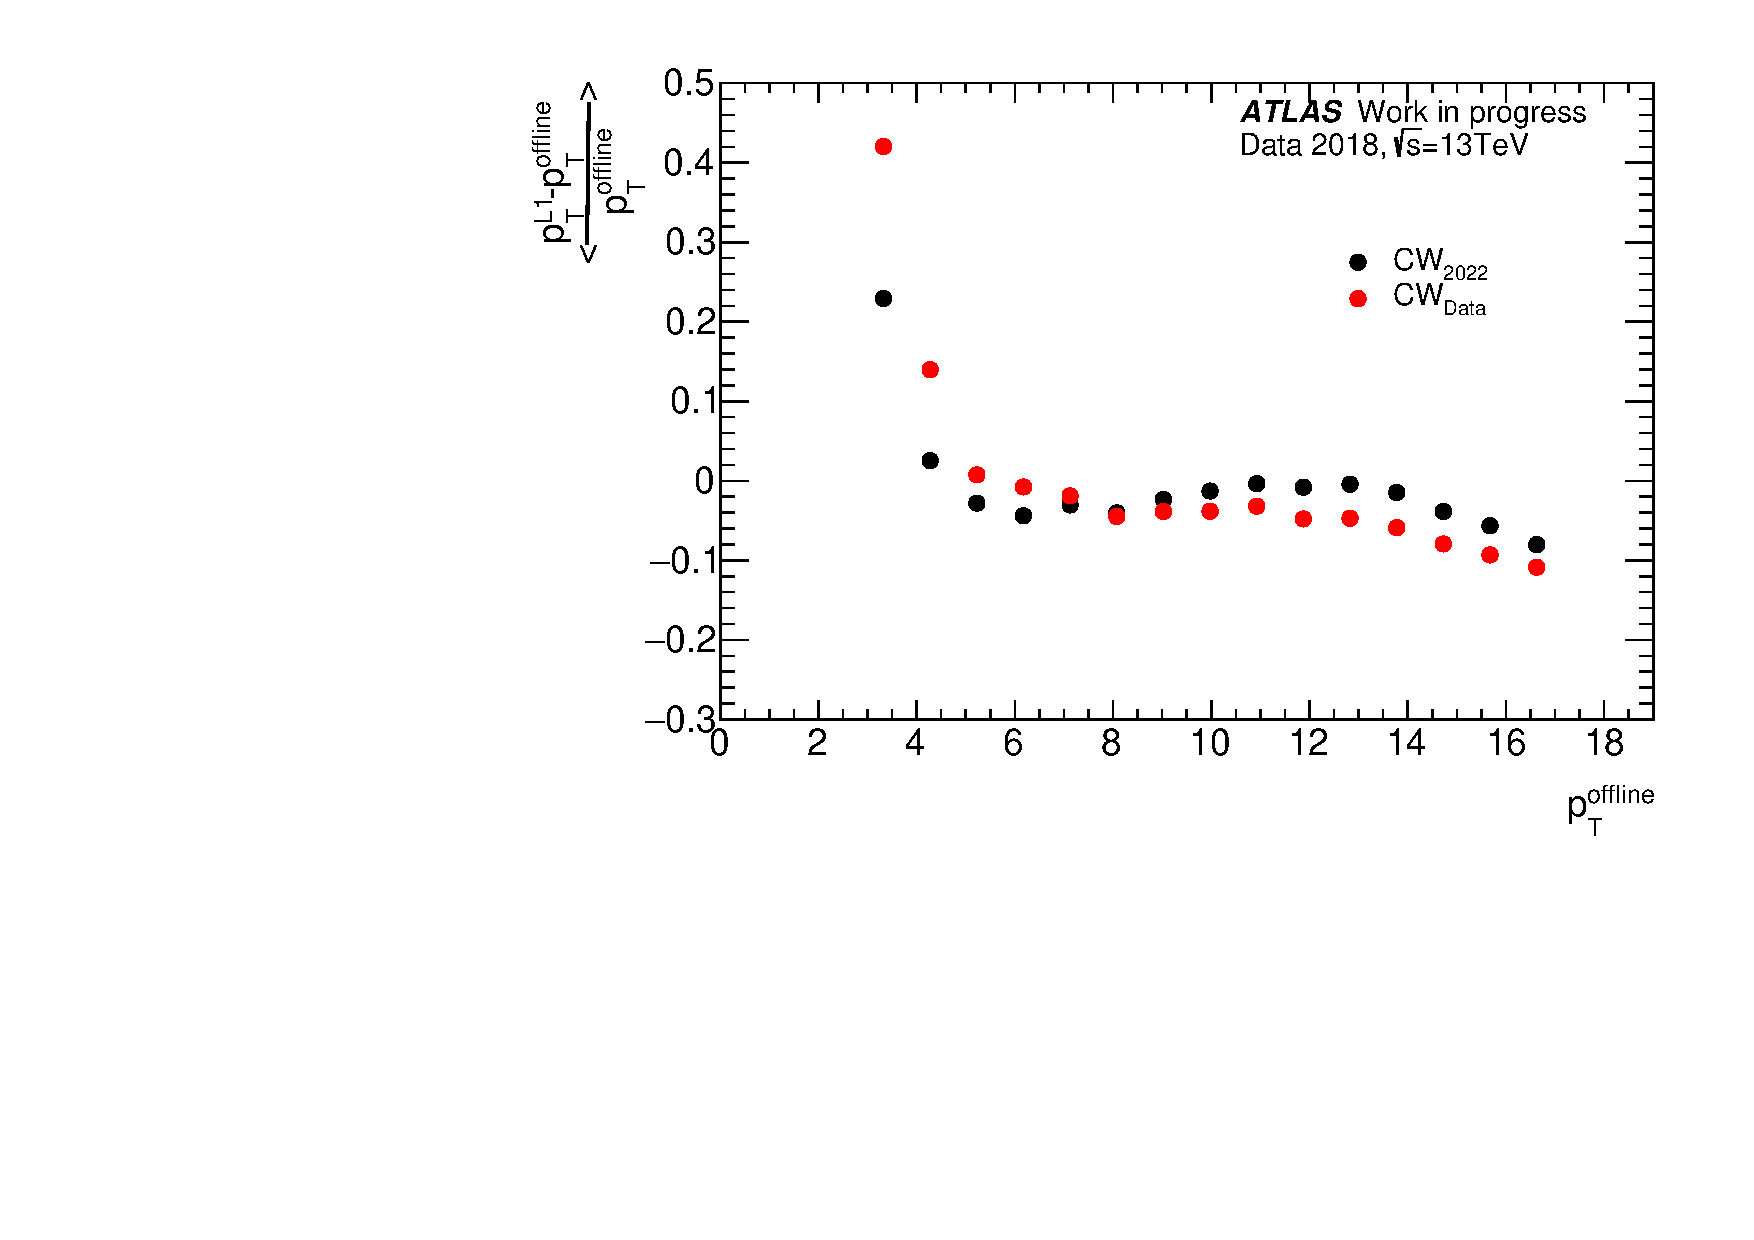
\includegraphics[clip, width=8cm]{fig/5/residual_mean_Data_re.pdf}
        %\vspace{5pt}
        \subcaption{Mean値}
        \label{fig:resi_mean_Data}
    \end{minipage}&
    %\hfill
    \begin{minipage}[b]{0.55\hsize}
        %\centering
        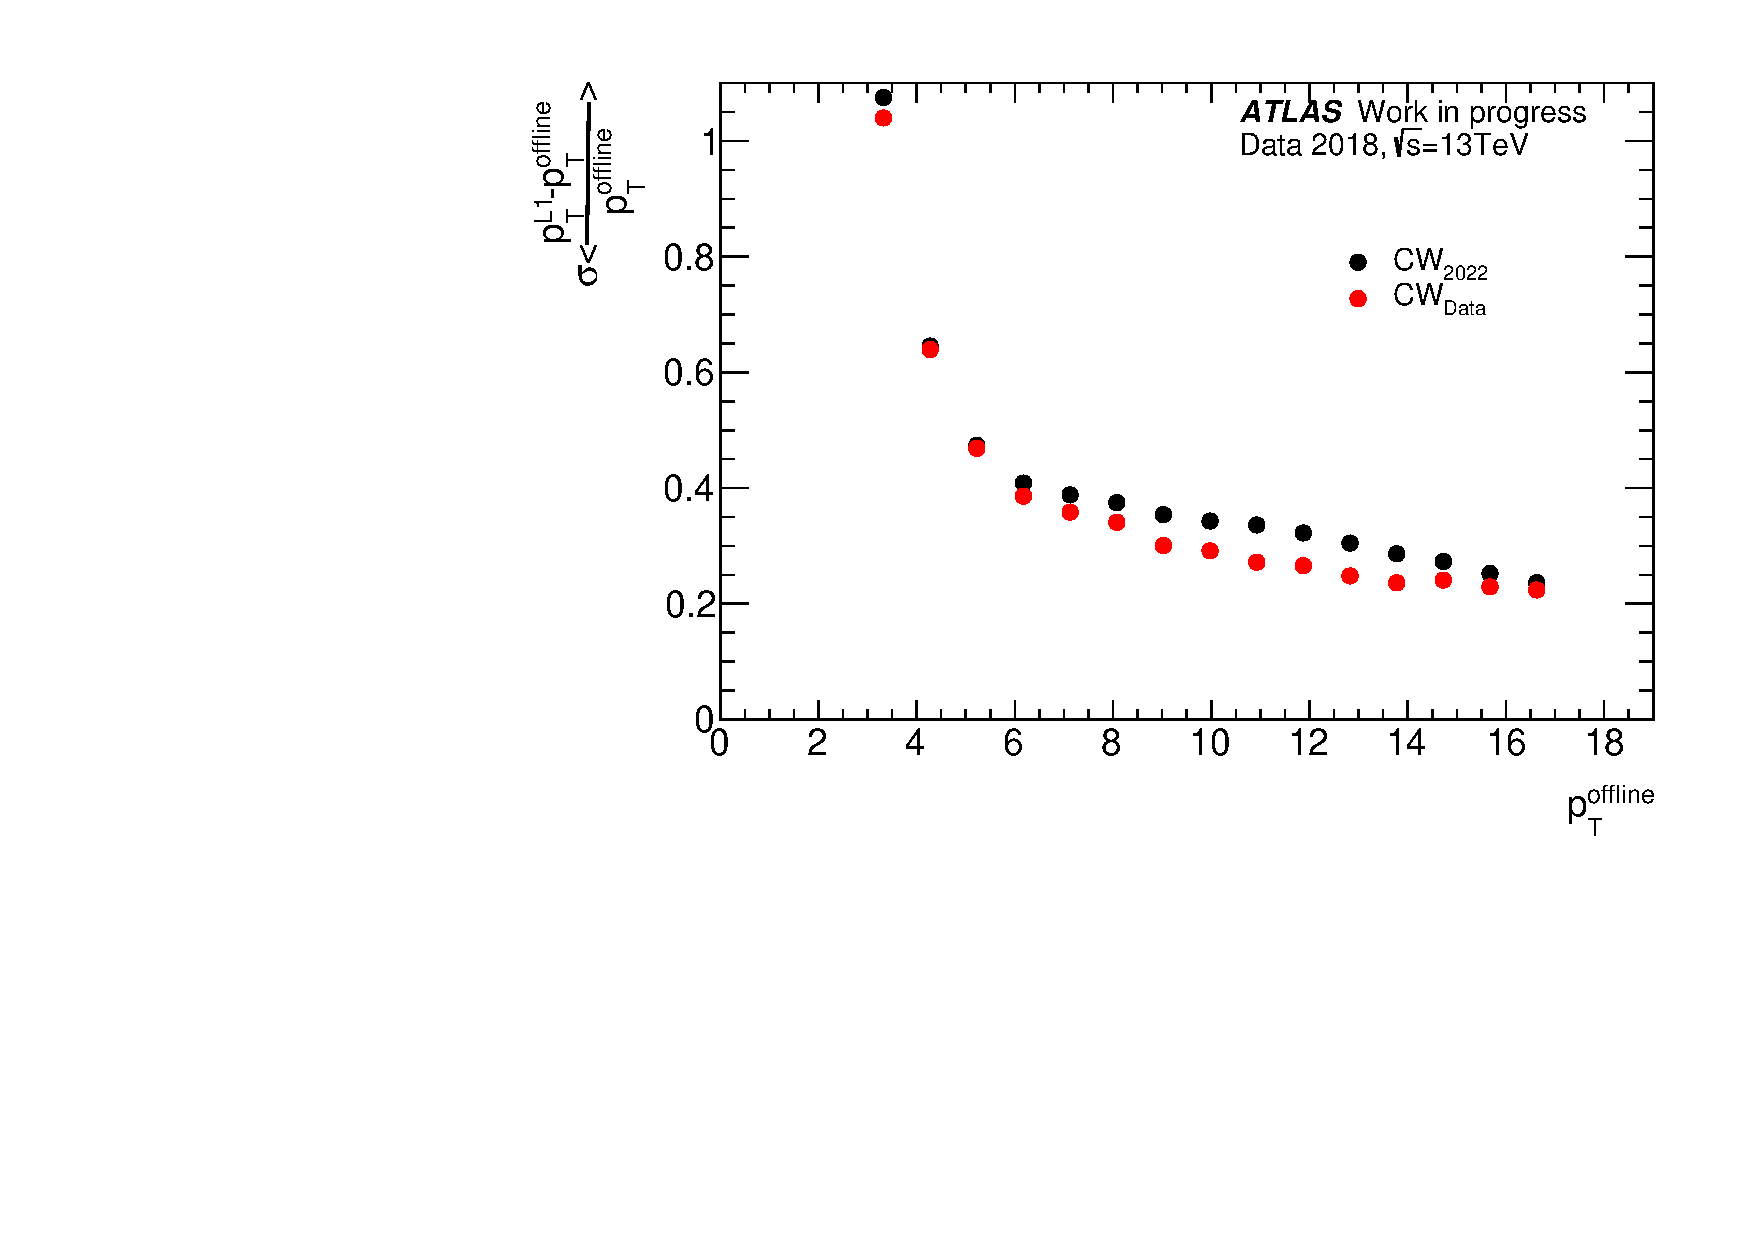
\includegraphics[clip, width=8cm]{fig/5/residual_stdDeVpdf_re.pdf}
        %\vspace{5pt}
        \subcaption{標準偏差}
        \label{fig:resi_std_Data}
    \end{minipage}
    \end{tabular}
    \caption{本研究の手法で作成した$\mathrm{CW_{Data}}$と2022年度Run-2で使用された$\mathrm{CW_{2022}}$の$p_{\rm{T}}$ residualの比較。}
    \label{residual_Data}
\end{figure}







\subsection{トリガーレートの評価}
次に、本手法で作成したCWを使用したときのトリガーレートの評価を行う。トリガーレートとは、実験データにおけるトリガーが発行された事象数である。
ここでは2016年のRun-2データを用いてトリガーレートを計算する。
Run-2データにはHLTでのプリスケールによるバイアスが存在するため、バイアスのない状態でトリガーレートを計算するために、「HLT$\_$noalg$\_$L1MU4」を要求する。このトリガーはL1トリガーにおいて$p_{\rm{T}}$閾値が4GeV以上を要求するが、HLTによる事象選別のない(Pass-through)トリガーチェインである。
その後、HLT$\_$noalg$\_$L1MU4が鳴ったイベントの中でL1$\_$MU$x$が鳴ったイベントがいくつ存在するかを調べ、ルミノシティが$2\times10^{43}$~cm$^{-2}$s$^{-1}$の時のL1$\_$MU4のトリガーレートをかけることでMU$x$のトリガーレートを見積もる。式~\eqref{equ:トリガーレート}にトリガーレートの計算式を示す。
\begin{equation}
    \rm{MU}xのレート[\rm{kHz}] = \frac{\rm{MU}xが鳴ったイベント数}{HLT\_noalg\_L1MU4が鳴った全イベント数}\times L1\_MU4のレート[kHz]
    \label{equ:トリガーレート}
\end{equation}
図~\ref{fig:Ratev05v06}に2016年で取得されたデータを用いて算出したトリガーレートを示す。

\begin{figure}[tb]
  \centering
  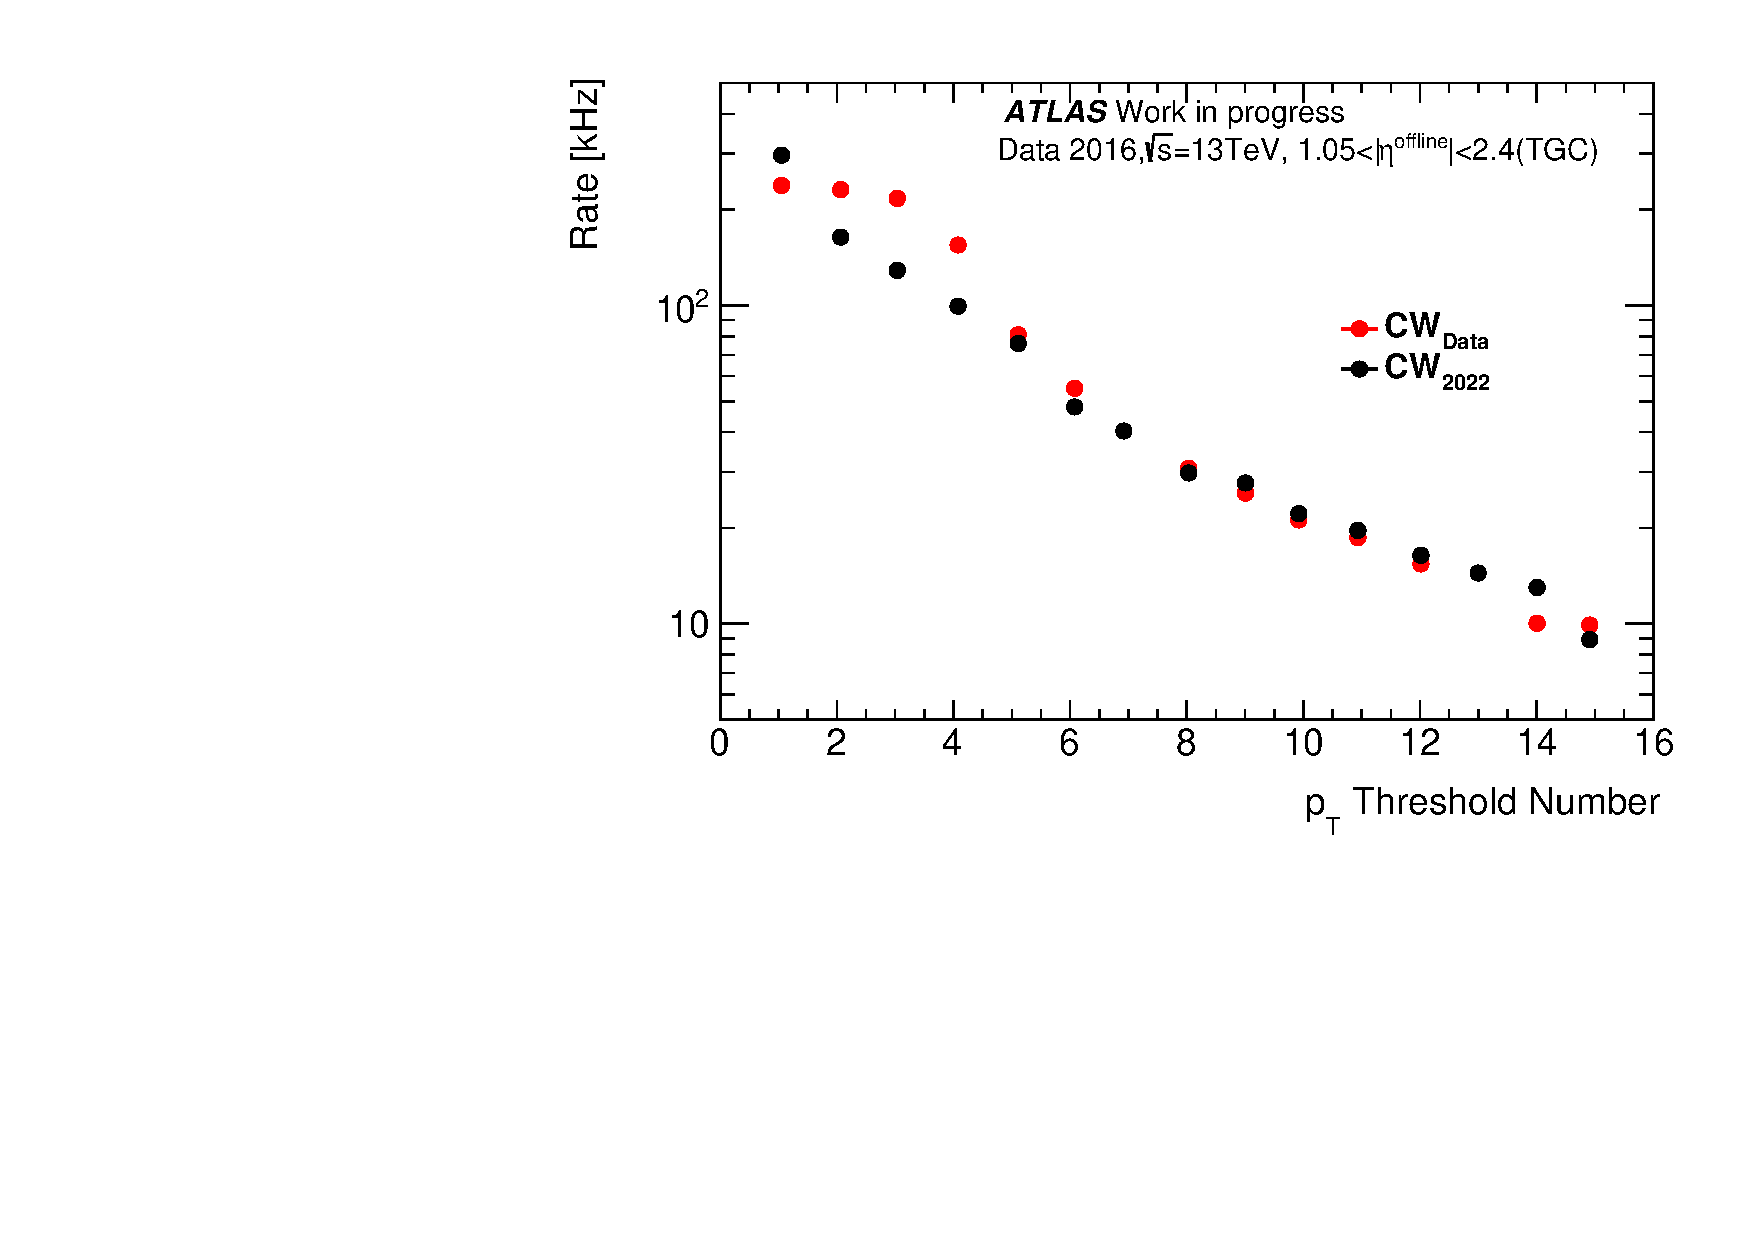
\includegraphics[clip, width=11cm]{fig/5/15rate_re.pdf}
  \caption{TGCにおけるシングルミューオンのトリガーレート。}
  \label{fig:Ratev05v06}
\end{figure}
プライマリートリガーである$p_{\rm{T}}$閾値14~GeVのトリガーレートは、本研究の手法で作成した$\mathrm{CW_{Data}}$では15~kHz、2022年度Run-2で使用された$\mathrm{CW_{2022}}$では16~kHzとなり、トリガーレートの削減が確認できた。また、$p_{\rm{T}}$閾値7~GeV以上のトリガーにおいて、$\mathrm{CW_{Data}}$のトリガーレートの値は$\mathrm{CW_{2022}}$と同等であることが見て取れる。
しかし、$p_{\rm{T}}$閾値4~GeV、5~GeV、6~GeVのトリガーに関してはトリガーレートの増加が見られた。
これはトレーニングデータに含まれる多重散乱の影響を受けた低い$p_{\rm{T}}$のミューオンによるものだと考えられる。シミュレーション上でも多重散乱を考慮してミューオンの運動をシミュレートしているが、完全に多重散乱の影響をシミュレーションできているわけではない。
そのため、シミュレーションデータには含まれていないような多重散乱したミューオンの影響で、$\mathrm{CW_{Data}}$における低い$p_{\rm{T}}$の判定領域が大きく広がったことが原因だと考えられる。
本研究で開発した手法では、$p_{\rm{T}}$閾値を柔軟に選択することができるため、トリガーレートの削減に焦点を置いた$p_{\rm{T}}$閾値の選択をすることでトリガーレートを抑えることのできるCWを作成可能である。

%そのため、シミュレーションデータから作成した$\mathrm{CW_{2022}}$と実際のデータから作成した$\mathrm{CW_{Data}}$を比較すると、$\mathrm{CW_{Data}}$の方が低い$p_{\rm{T}}$の判定領域が大きく広がっていることが原因だと考えられる。
%これは、\ref{fig:Effictive_thr_v1}で示したように、低いEffective~Threshouldへの変換ができていなことが原因で、低い$p_{\rm{T}}$閾値のトリガーの性能が悪くなってしまったと思われる。
%ただし、Run-3以降のエンドキャップ部のミューオントリガーでは\ref{section2-2-4}節で述べたようにNSWによるインナーコインシデンスが可能となり、トリガーレートの大幅な削減が見込まれている。そのため、本研究で作成したCWに対してもインナーコインシデンスを用いることで、$p_{\rm{T}}$閾値4~GeV、5~GeV、6~GeVのトリガーに関してもトリガーレートの削減が可能である。




\section{性能評価のまとめ}
本章では本研究の手法で作成したCWの評価を行った。

まず、本研究の手法で期待される機械学習による最適化の評価を行った。
ミューオンの電荷別にトリガー効率を算出したところ、2022年Run-3で使用された$\mathrm{CW_{2022}}$で見られたトリガー効率の電荷依存が、本研究の手法で作成したCWでは見られなくなった。このことから、検出器アライメントの最適化が行えていることが確認できた。

次に、15段階のトリガー効率の評価を、Turn-on CurveのPlateau EfficiencyとResolutionといった観点から評価を行っ結果、本研究の手法で作成した2種類のCWは$\mathrm{CW_{2022}}$のTurn-on Curveと比べてトリガー効率の向上が確認できた。
また、L1Muonのプライマリートリガーである$p_{\rm{T}}$閾値14~GeVのトリガー効率について、$\mathrm{CW_{2022}}$はトリガー効率が85.4$\%$であったのに対し、$\mathrm{CW_{Data}}$ではトリガー効率が86.7$\%$となったことから約1$\%$の向上が確認できた。

さらに、$p_{\rm{T}}$判定精度の評価を$p_{\rm{T}}$ residualを計算することで評価を行った。
本研究の手法で作成したCWは、$\mathrm{CW_{2022}}$と比べて判定精度の向上がみられる。しかし、低い$p_{\rm{T}}$における$p_{\rm{T}}$ residualでは、mean値が悪くなっている。一方でResolutionを比べると改善されていることから、機械学習の出力からの$p_{\rm{T}}$閾値の選択方法を変更することによって低い$p_{\rm{T}}$における判定精度の向上が見込まれる。

最後に、トリガーレートの評価を行った。
プライマリートリガーである$p_{\rm{T}}$閾値14~GeVのトリガーレートは、本研究の手法で作成した$\mathrm{CW_{Data}}$では約15~kHz、2022年度Run-2で使用された$\mathrm{CW_{2022}}$では約16~kHzとなり、トリガーレートの削減が確認できた。また、$p_{\rm{T}}$閾値7~GeV以上のトリガーにおいて、$\mathrm{CW_{Data}}$のトリガーレートの値は$\mathrm{CW_{2022}}$と同等であることが見て取れる。
しかし、$p_{\rm{T}}$閾値6~GeV以下のトリガーにおいてはトリガーレートの増加がみられた。これはシミュレーションでは表現しきれないような多重散乱したミューオンの影響によるものだと考えられる。

以上より、本研究の手法である機械学習を用いた手法は、従来の手法と同様に15段階の閾値を持ったCWの作成を可能とし、さらに検出器アライメントに対する補正を自動的に行えることが確認できた。
本研究の手法では将来、検出器やシステムのアップグレードが行われた際に本研究の手法が有効である。


%\begin{figure}[htbp]
%    %\centering
%    \begin{tabular}{cc}
%    \begin{minipage}[b]{0.45\hsize}%
%        %\centering
%        \hspace*{-1cm}
%        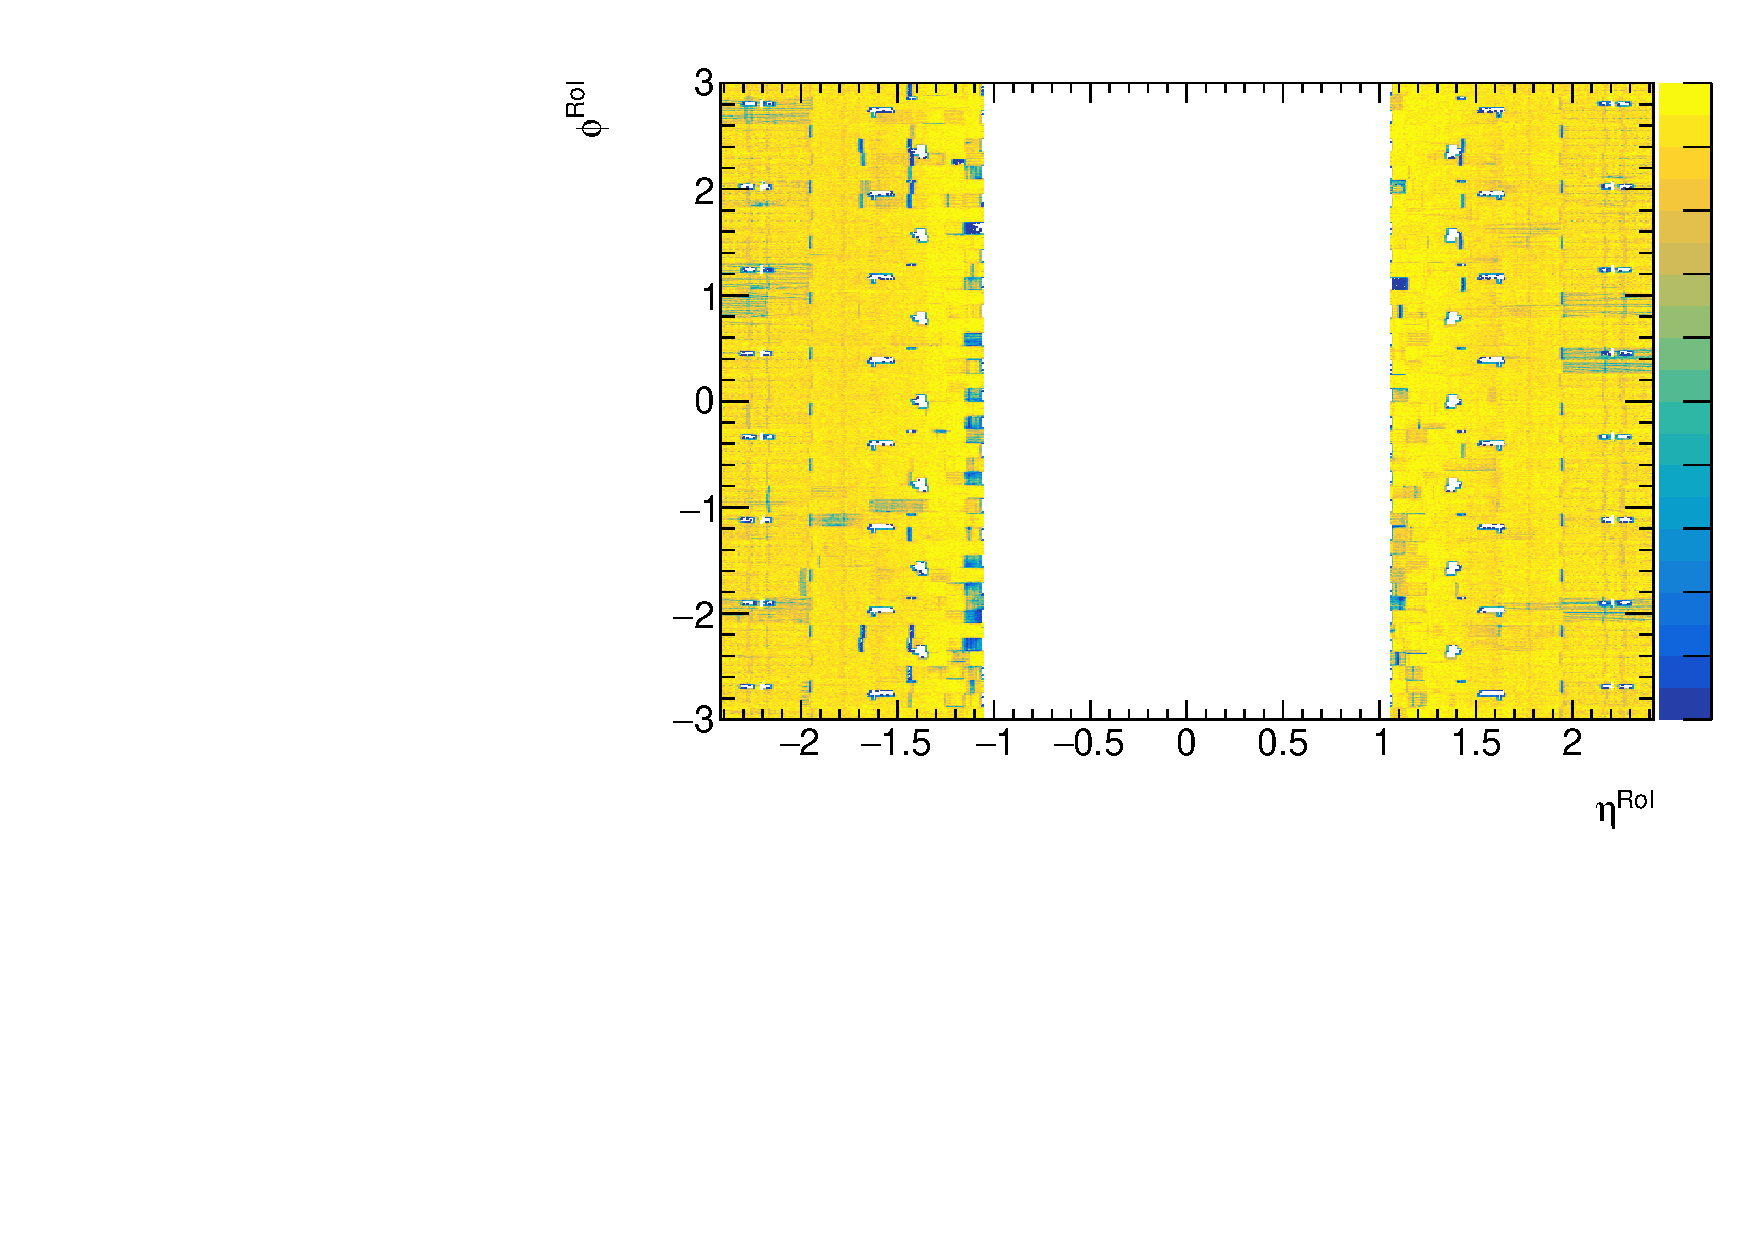
\includegraphics[clip, width=7cm]{fig/5/h2_Data14_Eff.pdf}
%        %\vspace{5pt}
%        \subcaption{}
%        \label{fig:dataEffMU14}
%    \end{minipage}%
%    %\hfill
%    \begin{minipage}[b]{0.55\hsize}%
%        %\centering
%        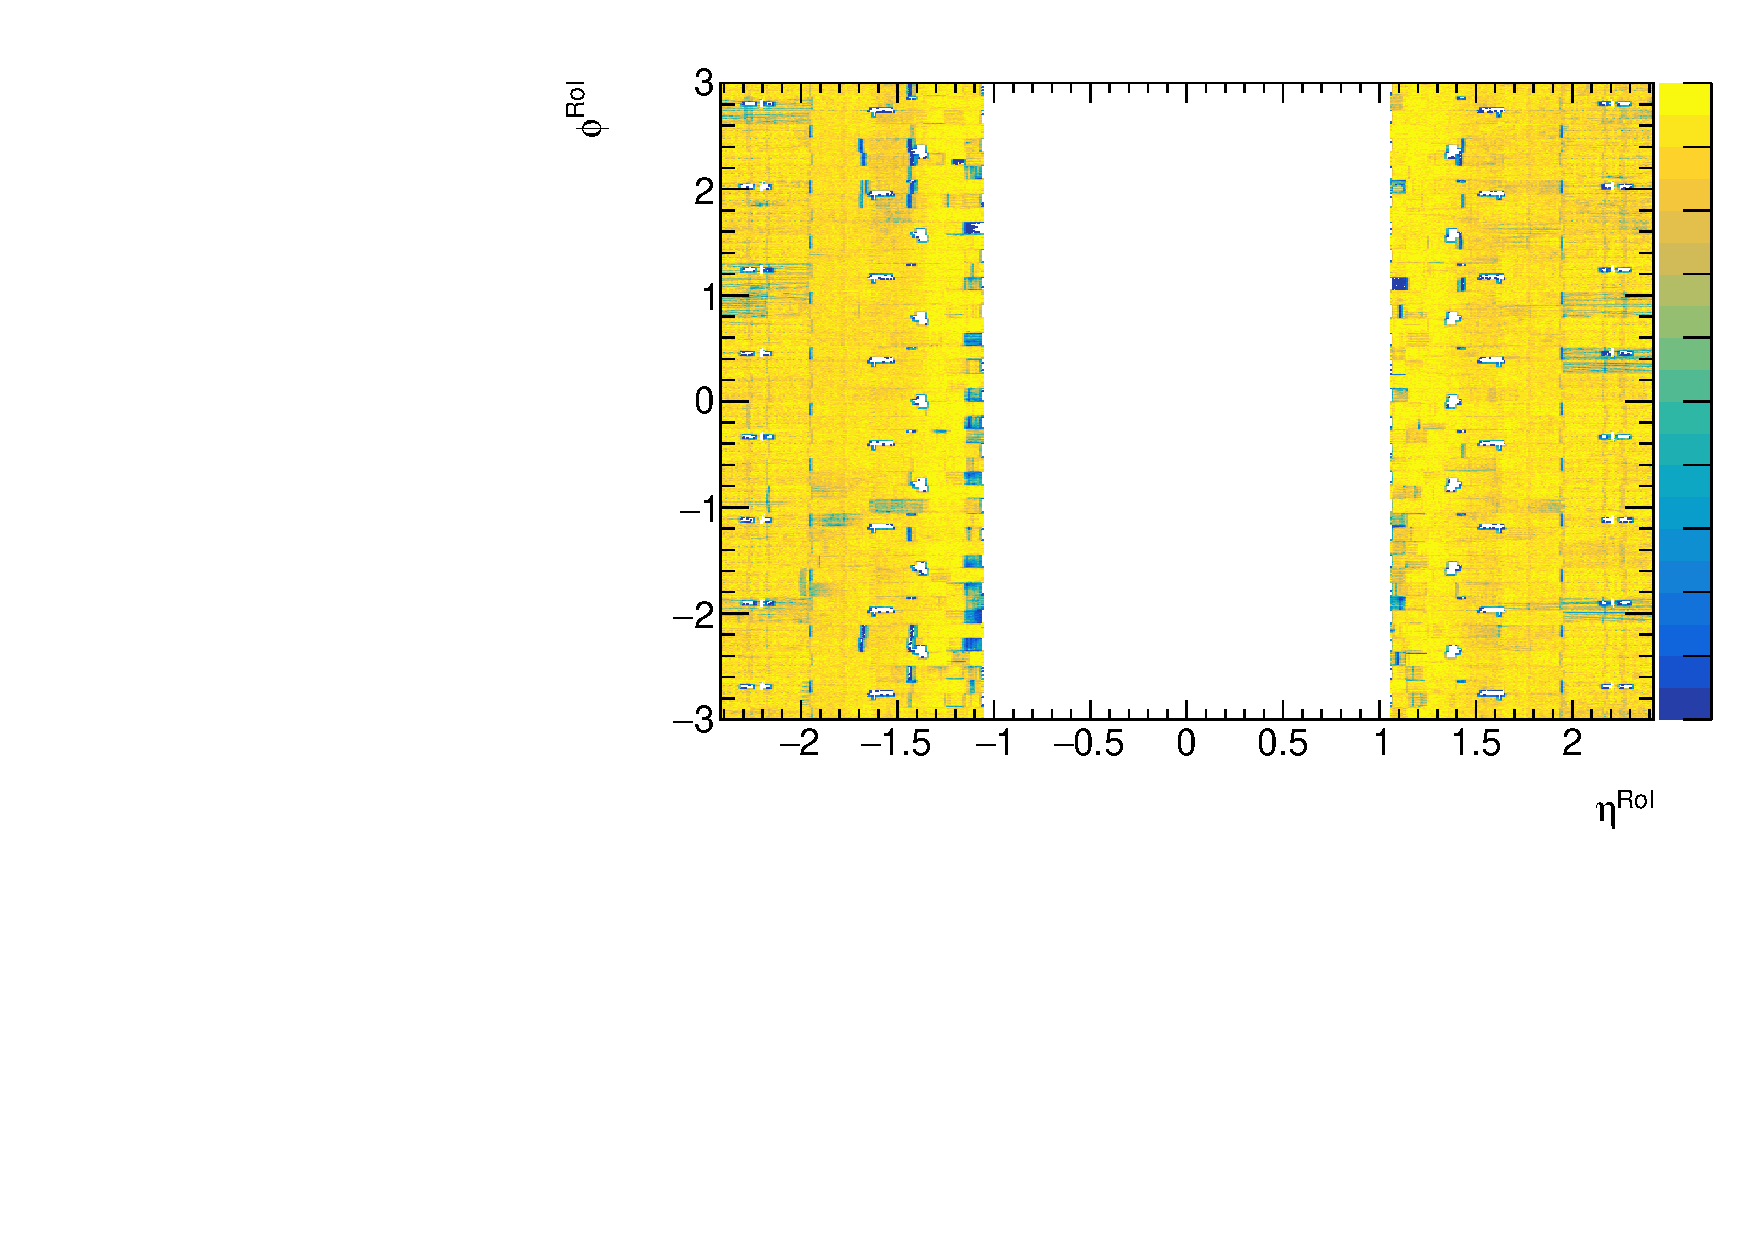
\includegraphics[clip, width=7cm]{fig/5/h2_v0514_Eff.pdf}
%        %\vspace{5pt}
%        \subcaption{}
%        \label{fig:v05EffMU14}
%    \end{minipage}%
%    \end{tabular}
%    \caption{TGCのRoIにおけるトリガー効率。分母を$p_{\rm{T}}$が20~GeV以上のオフライン再構成されたミューオンとし、その中で$p_{\rm{T}}$閾値14~GeVのトリガーを鳴らしたミューオンの割合を表している。(a):$\mathrm{CW_{Data}}$(b):$\mathrm{CW_{2022}}$}
 %   \label{EffMU14}
%\end{figure}



%低い$p_{\rm{T}}$閾値のトリガーに対しての課題があるが、トレーニングデータの低い$p_{\rm{T}}$のミューオン数を増加させることや、適切な重みをつけてトレーニングを行うことで、
